 A basic event selection is made to enhance the signal-like events and is discussed in \Sec{sec:trig}. The necessary  corrections in order to make simulation and data coherent, introduced in \Chap{chap:4}, are summarised in \Sec{sec:SummaryCor} and the resulting data/MC agreement is shown in \Sec{sec:corrections}. The reconstruction of the physics objects in the event is discussed in \Sec{sec:recon}. One of the main background processes entering the analysis are background processes that have prompt leptons contaminated by other leptons. These contaminating leptons originate either from real lepton from decays of tau leptons or from hadronized mesons or baryons
 (so-called ``non-prompt leptons''), or originate from hadrons or jets misidentified as leptons (so-called ``fake leptons'').  These two classes  of contamination together will be referred to as the not prompt-lepton (\NPL) background. The \NPL\ background  is
 evaluated with a data-driven method discussed in \Sec{sec:NPL}. The analysis strategy is presented in \Sec{sec:regions}, where selection criteria are defined to create signal and background regions to constrain the huge \SM\ background compared to the expected signal. %https://indico.cern.ch/event/283659/contributions/643371/attachments/523063/721480/davidcurtin_fakeleptonsim_MC4BSM_23may2014_v1.key.pdf

\section{Baseline event selection and filters}
\label{sec:trig}
 In this analysis a search is performed in a final state made up of a \PZ\ boson and a top quark, associated or not with a jet. The leptonic decay of the \PZ\ boson and the top quark is considered for which the leading order Feynman diagrams can be seen in \fig{fig:feynST} and \fig{fig:feynTT}. 
 The signal consists of the single top quark production through a FCNC \tZq\ interaction (\tZ\ in the final state) and the top quark pair production where one of the top quarks decays through the FCNC \tZq\ vertex (\tZq\ with $\Pquark= \Pcharm, \Pup$ in the final state). Their final state signatures consist of three leptons, only considering electrons or muons, and a jet originating from a \Pbottom\ quark. For \FCNC\ \tZq, there is an additional up or charm jet. Leptons from tau decays are not vetoed and are entering the analysis via their leptonic decays. Four different three-lepton channels based on lepton flavour are considered: \eee, \eemu, \emumu, and \mumumu.
\begin{figure}[htbp]
	\centering
	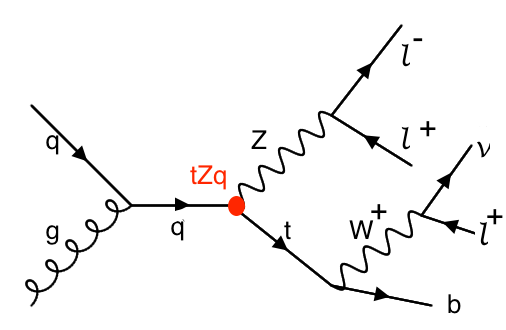
\includegraphics[width=0.45\linewidth]{5_EventSelection/Figures/feynmanST}
	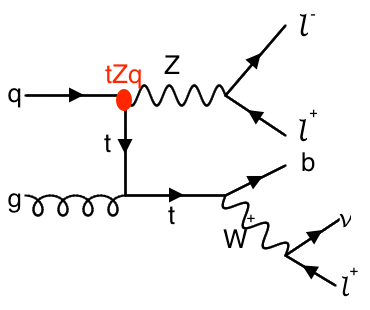
\includegraphics[width=0.35\linewidth]{5_EventSelection/Figures/FeynmanSTtzq}
	\caption{Single top quark Feynman diagrams at leading order. The vertex labelled \tZq\ is the sought-for \FCNC\ interaction.}
	\label{fig:feynST}
\end{figure}
\begin{figure}[htbp]
	\centering
	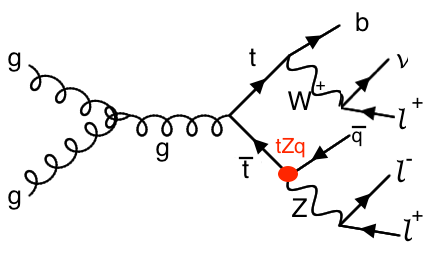
\includegraphics[width=0.45\linewidth]{5_EventSelection/Figures/FeynmantttZq}
	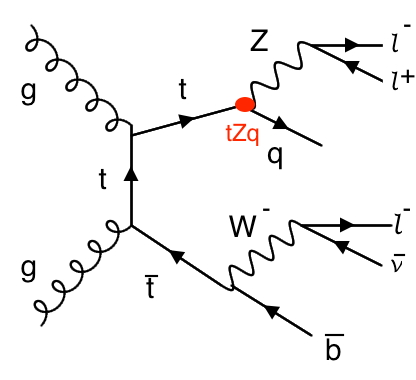
\includegraphics[width=0.35\linewidth]{5_EventSelection/Figures/FeynmantttZq2}
	\caption{Top quark pair Feynman diagrams at leading order. The vertex labelled \tZq\ is the sought-for \FCNC\ interaction. }
	\label{fig:feynTT}
\end{figure}
  

The CMS collaboration recorded in the course of 2016, proton collisions data at a centre-of-mass of 13 \TeV\ with a total recorded integrated luminosity of $35.9~\fbinv$. The baseline event selection has as goal to substantially reject \SM\ background events, whilst maintaining a high signal efficiency. The CMS trigger system, described in \Sec{sec:DAQ}, filters out the main fraction of the collision events from uninteresting processes, and dedicated trigger paths are defined to single out the events with the required detector signature for the search presented in  this thesis.

 The trigger paths are chosen based on online trigger objects with at least one muon (M), at least one electron (E), at least two muons (MM), at least two electrons (EE), at least one muon and an electron (ME), at least three muons (MMM), at least three electrons (EEE), at least two muons and one electron (MME), or at least two electrons and one muon (EEM). For the MC simulation a simple $or$ of all triggers is taken, hence the event is considered when it passes one of the trigger paths. For data however, double counting of the same event has to be taken into account and a procedure to avoid double counting has been put into place. This procedure consists of vetoing in a given dataset the events that are already selected in another, as given in \tab{tab:triggerlogic}. 


  For the single lepton triggers, at least one electron (muon) with a transverse momentum \pt\ higher than $32\: (24)~\GeV$ is required.  The dilepton triggers require the combination of an electron (muon) with $\pt >\: 23~\GeV$ and a muon (electron) with $\pt > 8~\GeV$, or the combination of an electron (muon) with $\pt > 23\: (17)~\GeV$ and an electron (muon) with $\pt > 12\:(8)~\GeV$. Events collected by the trilepton triggers require a combination of an electron (muon) with $\pt > 16\:(12)~\GeV$, a second electron (muon) of  $\pt > 12\:(10)~\GeV$,  and a third electron (muon) with $\pt > 8\:(5)~\GeV$. The mixed trilepton trigger events require a combination of two electrons (muons) with $\pt > 12\:(9)~\GeV$ and a third muon (electron) with $\pt > 8\:(9)~\GeV$. The HLT trigger paths used in data and simulation are summarised in \tab{tab:Trigger}. 
  \begin{table}[htbp]
  	\centering
  	\caption{Trigger logic used to select data events in order to avoid double counting.}
  	\begin{tabular}{ll}
  		\toprule
  		Dataset & Trigger Logic \\ 
  		\midrule
  		\emu & EM $\Arrowvert$ EEM $\Arrowvert$ MME \\ 
  		
  		\mumu & (MM $\Arrowvert$ MMM) \&\& !( EM $\Arrowvert$ EEM $\Arrowvert$ MME)  \\ 
  		
  		\ee & (EE $\Arrowvert$ EEE) \&\& !(MM $\Arrowvert$ MMM) \&\& !( EM $\Arrowvert$ EEM $\Arrowvert$ MME) \\ 
  		
  		single \Pmu & M \&\& !(EE $\Arrowvert$ EEE) \&\& !(MM $\Arrowvert$ MMM) \&\& !( EM $\Arrowvert$ EEM $\Arrowvert$ MME) \\ 
  		
  		single e & E \&\& !M \&\& !(EE $\Arrowvert$ EEE) \&\& !(MM $\Arrowvert$ MMM) \&\& !( EM $\Arrowvert$ EEM $\Arrowvert$ MME)  \\ 
  		\bottomrule
  	\end{tabular} 
  	\label{tab:triggerlogic}
  \end{table}
\begin{table}[htbp]
	\centering
	\caption{HLT trigger paths used to select data and simulation events.}
	\begin{tabular}{lc}
		\toprule
		Trigger path name &  Trigger type \\ 
		\midrule
		HLT\_Mu23\_TrkIsoVVL\_Ele8\_CaloIdL\_TrackIdL\_IsoVL\_v &  ME \\ 
		%		\hline 
		HLT\_Mu23\_TrkIsoVVL\_Ele8\_CaloIdL\_TrackIdL\_IsoVL\_DZ\_v &  ME \\ 
		%		\hline 
		HLT\_Mu8\_TrkIsoVVL\_Ele23\_CaloIdL\_TrackIdL\_IsoVL\_v &  ME \\ 
		%		\hline 
		HLT\_Mu8\_TrkIsoVVL\_Ele23\_CaloIdL\_TrackIdL\_IsoVL\_DZ\_v &  ME \\ 
		%		\hline 
		HLT\_DiMu9\_Ele9\_CaloIdL\_TrackIdL\_v &  MME \\ 
		%		\hline 
		HLT\_Mu8\_DiEle12\_CaloIdL\_TrackIdL\_v &  EEM \B \\ 
		\hdashline
		HLT\_IsoMu24\_v &  M \T  \\ 
		%		\hline 
		HLT\_IsoTkMu24\_v &  M \B \\ 
		\hdashline
		HLT\_Ele32\_eta2p1\_WPTight\_Gsf\_v &  E \T \B  \\ 
		\hdashline
		HLT\_Mu17\_TrkIsoVVL\_Mu8\_TrkIsoVVL\_v &  MM \T \\ 
		%		\hline 
		HLT\_Mu17\_TrkIsoVVL\_TkMu8\_TrkIsoVVL\_v &  MM \\ 
		%		\hline 
		HLT\_Mu17\_TrkIsoVVL\_Mu8\_TrkIsoVVL\_DZ\_v &  MM \\ 
		%		\hline 
		HLT\_Mu17\_TrkIsoVVL\_TkMu8\_TrkIsoVVL\_DZ\_v &  MM \\ 
		%		\hline 
		HLT\_TripleMu\_12\_10\_5\_v &  MMM \B \\ 
		\hdashline
		HLT\_Ele23\_Ele12\_CaloIdL\_TrackIdL\_IsoVL\_DZ\_v &  EE \T \\ 
		HLT\_Ele16\_Ele12\_Ele8\_CaloIdL\_TrackIdL\_v &  EEE \\ 
		\bottomrule 
	\end{tabular} 
	\label{tab:Trigger}
\end{table}

In order to ensure a full trigger efficiency, the offline \pt\ thresholds are set higher than the online trigger thresholds. 
Selected offline electrons (muons) are required to have a $\pt>35~(30)~\GeV$ and $|\eta| < 2.1~(2.4)$. The electrons and muons corresponding to a tight working point, as discussed in \Sec{sec:MuonID} (\tab{tab:MuonReq}) and \Sec{sec:ElectronID} (\tab{tab:ElecReq}), are used for analysis. Only events with exactly three leptons are being considered for the analysis. Events with extra leptons according to looser working points,  as discussed in \Sec{sec:MuonID} (\tab{tab:MuonReq}) and \Sec{sec:ElectronID} (\tab{tab:ElecReq}), are vetoed. The trigger efficiency estimation is described in \Sec{sec:triggereff} and is approximately 100\%. To ensure that all reconstructed particles considered for the analysis are corresponding to a proton interaction and to remove signals from beam halo particles as well as detector noise, several filters are used. These are described in \Sec{sec:Filters}. In addition to three leptons, the selected events should at least contain one offline jet with a  $\pt > 30~\GeV$ and $|\eta| < 2.4$, for which at least one jet is tagged as coming from a \Pbottom\ quark (so-called b-tagged jet or b jet). 


\subsection{Event cleaning}
\label{sec:Filters}
 %%met filter %http://cds.cern.ch/record/2205284/files/JME-16-004-pas.pdf

Some events arising from instrumental noise and beam backgrounds might end up in the data~\cite{Filters,CMS-PAS-JME-16-004}. In the ECAL, spurious deposits can appear from non-collision origins such as beam halo particles, or from particles hitting the sensors in the ECAL photo-detectors. Conjointly, dead ECAL cells can cause artificial missing transverse energy. The HCAL can also show spurious energy from particle interactions with the light guides and the photomultiplier tubes of the HF, as well as noisy hybrid photodiodes. In CMS, different algorithms, so-called filters, are developed to identify and suppress these events. 


The ECAL electronics noise and spurious signals from particle interactions with photo detectors are mostly removed via topological and timing-based selections using only the ECAL information. The remaining effects such as anomalously high energy crystals and the lack of information for channels due to inefficiencies in the read-out are removed through dedicated events filters. Five ECAL endcap supercrystals have been identified for giving anomalously high energies due to high amplitude pulses in several channels at once, and are masked. Furthermore, the crystal read-out from a small amount of ECAL towers is not available. Nonetheless, their trigger primitive information is still available making it possible to estimate the magnitude of unmeasured energy and when the value is too large, the event is filtered out. 

The machine induced particles via for example beam-gas, or beam-pipe interactions, that are flying with the beam, affect the physics analysis. They leave a calorimeter deposit along a line at constant $\phi$ in the calorimeter, and interactions in the CSCs will often line up with this deposit. This can be seen in \fig{fig:beamhalo}. Therefore, events containing such beam halo particles are removed from the selection with the CSC Beam Halo Filter. This algorithm uses information related to the geometric quantities, energy deposits, and timing signatures. For 2016 proton collision data, the filter rejects 85\% in a halo-enriched sample, whereas the mistag probability determined from simulation is found to  be less than 0.01\%~\cite{CMS-PAS-JME-16-004}.  
\begin{figure}[htbp]
	\centering
	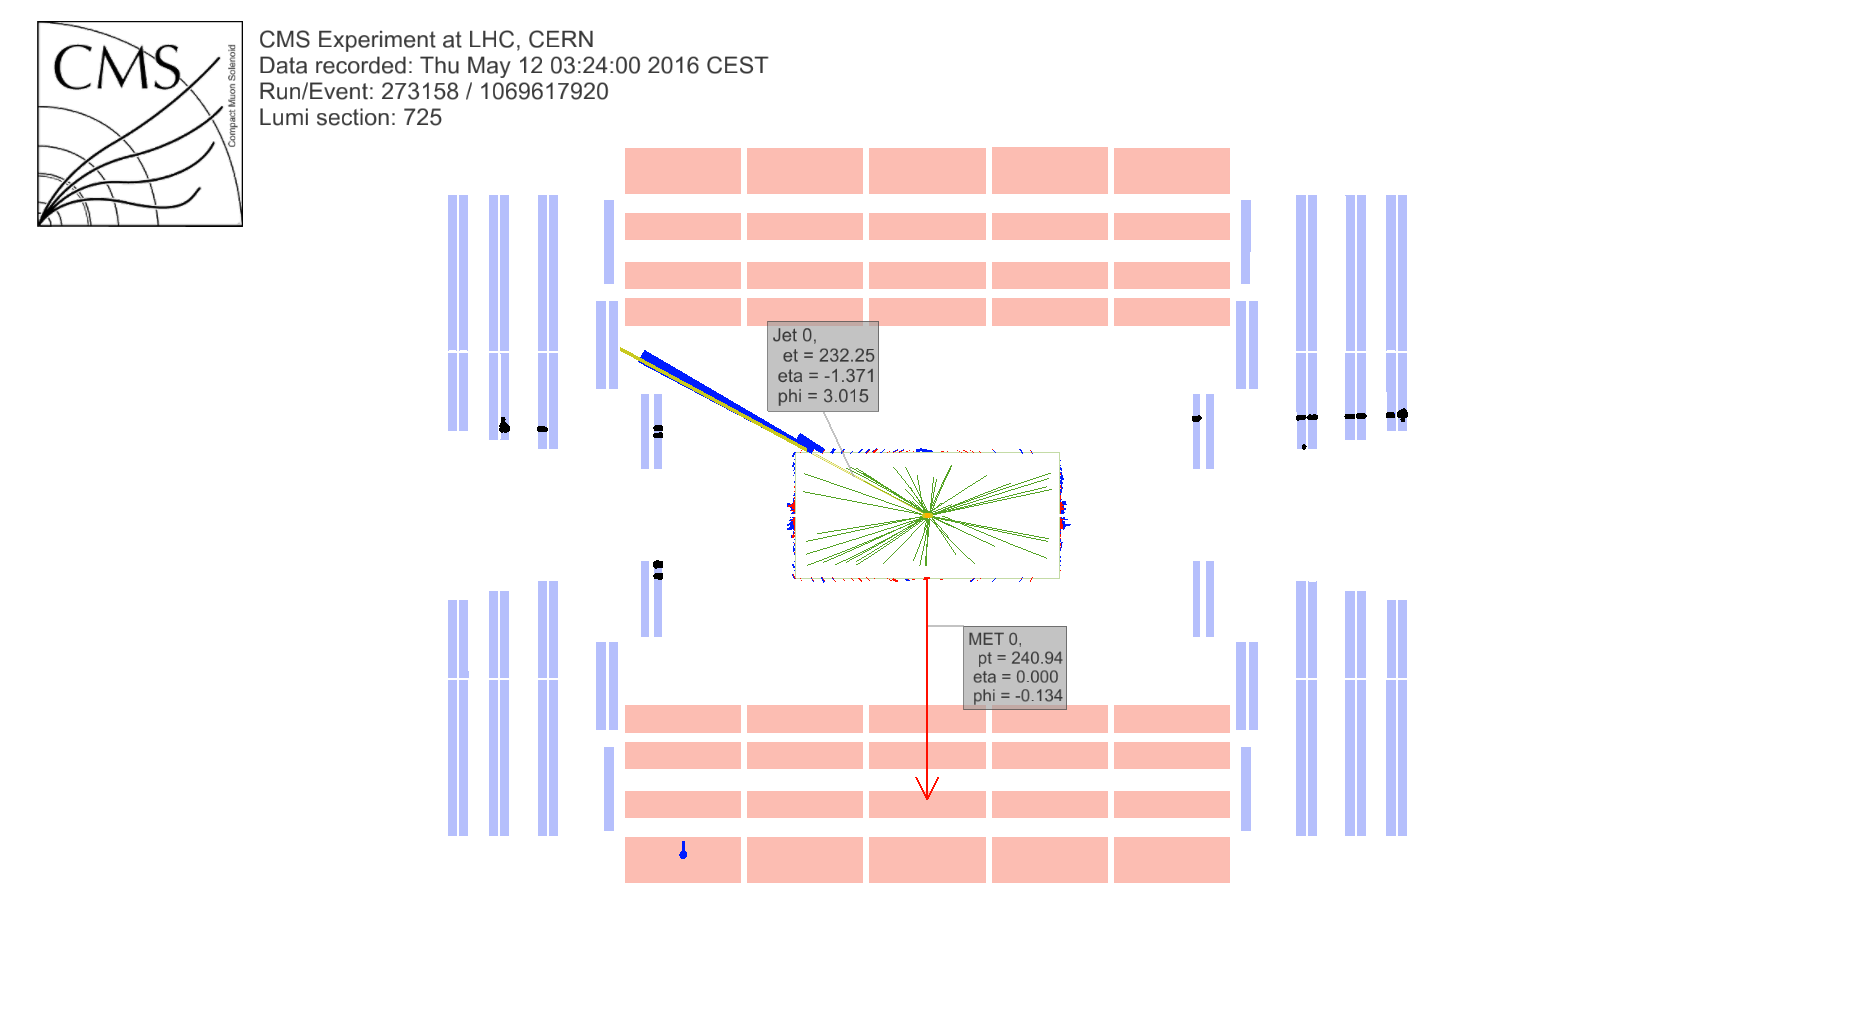
\includegraphics[width=.7\linewidth]{5_EventSelection/Figures/Figure_004}
	\caption{Event display of a beam halo event with collinear hits in the CSC (black), missing transverse energy of 250 \GeV\, and a jet of 232 \GeV. The hadronic deposit is spread in $\eta$, but narrow in $\phi$. Figure taken from~\cite{CMS-PAS-JME-16-004}. }
	\label{fig:beamhalo}
\end{figure}

Furthermore, there is anomalous high missing transverse energy coming from muons that lead to high-\pt\ tracks, but are considered not good by the particle flow algorithm. These low quality tracks will be  mislabelled as charged hadrons and will therefore be used in the calculation of the missing transverse energy. By investigating the purity of the reconstructed tracks and the relative transverse momentum error of the muons, these events can be filtered out. 


% see https://indico.cern.ch/event/591506/contributions/2387636/attachments/1381281/2099935/2016_12_01_MET_Scanning_Report_PPD.pdf
% see https://indico.cern.ch/event/537458/contributions/2184619/attachments/1281045/1903148/met_scanner_report_may30.pdf
% see https://indico.cern.ch/event/534040/contributions/2178680/attachments/1280427/1901837/HCALnoise_JamboreeMeeting_27May2016.pdf
%see https://indico.cern.ch/event/518559/contributions/2132815/attachments/1264581/1871184/beamhalostatus.pdf
% see https://twiki.cern.ch/twiki/bin/viewauth/CMS/MissingETOptionalFiltersRun2



\subsection{Estimation of the trigger efficiency}
\label{sec:triggereff}
The trigger efficiency in data is estimated using a data sample collected using unprescaled \Etmis\ triggers. These allow events 
with a combination of the missing transverse energy being higher than 110~\GeV~(120~\GeV) and the scalar sum of the transverse momenta of the reconstructed PF jets  $H_{\mathrm{T}}^{\mathrm{trig.}}$ being at least 300~\GeV~(120~\GeV), or events for which the calorimeter (PF) \Etmis\ is higher than 200~\GeV~(300~\GeV). For an HB-HE cleaned event, the PF missing transverse energy threshold is lowered to 170~\GeV.  These trigger paths are summarised in \tab{tab:METtrig} and chosen to be completely uncorrelated with the lepton triggers given in \tab{tab:Trigger}. 
\begin{table}[htbp]
		\centering
		\caption{Unprescaled \Etmis\ HLT trigger paths for estimating the trigger efficiency. An \textit{or} of the triggers is used to select events.}
		\begin{tabular}{cc}
			\toprule
			Trigger path  & Requirement \\
			\midrule
	 HLT\_PFHT300\_PFMET110\_v* & PF \Etmis > 110~\GeV, PF $H_{\mathrm{T}}^{\mathrm{trig.}}$ > 300 \GeV \\
	 HLT\_MET200\_v* & calorimeter \Etmis > 200~\GeV  \T \\
	HLT\_PFMET300\_v* & PF \Etmis > 300 \GeV  \T \\
 \multirow{2}{*}{HLT\_PFMET120\_PFHT120\_IDTight\_v*} & PF \Etmis > 120~\GeV, and \T \\
  &  PF $H_{\mathrm{T}}^{\mathrm{trig., tight WP}}$ > 120~\GeV \T \\
	  \multirow{2}{*}{HLT\_PFMET170\_HBHECleaned\_v*} & PF \Etmis > 170~\GeV,  cleaned for \T \\
	  &  HB/HE anomalous signals \T \\
	 \bottomrule
	 \end{tabular}
 \label{tab:METtrig}
\end{table}

The trigger efficiency is studied for the main background, namely \WZ+jets, with all corrections applied. For this study, the events passing a three-lepton cut and at least one jet, are being used. The corresponding efficiencies are then calculated as
\begin{equation}
\epsilon_{data} = \frac{\textnormal{Nb. of events passing lepton and MET triggers}}{\textnormal{Nb. of events passing MET triggers}}
\end{equation}
\begin{equation}
\epsilon_{MC} = \frac{\textnormal{Nb. of events passing lepton triggers}}{\textnormal{Nb. of total events}}
\end{equation}
The resulting efficiencies for all lepton channels combined are shown in \tab{tab:triggeff} and scale factors can be found in  \tab{tab:trigSFe}, where the scale factors are defined as 
\begin{equation}
SF = \frac{\epsilon_{data}}{\epsilon_{MC}}.
\end{equation} 
More detailed scale factors and efficiencies can be found in \App{app:TriggerSF}.
\begin{table}[htbp]
	\centering
	\caption{Trigger efficiencies on data events selected with \Etmis\ triggers and \WZ\ simulation for all three-lepton channels together. The unweighted number of events is quoted. Region A contains events after requiring three leptons and at least one jet. Region B has the same requirements as region A, but only events with exactly one jet that is b-tagged are considered. Region C also contains the requirements in region A, where at least one jet should be b-tagged. In region D, no events with a b-tagged jet are allowed.}
	\begin{tabular}{cccc}
		\toprule
		Region & {data} & &  {WZ simulation} \\ 
		& $\mathrm{N}_{\mathrm{selected}}/\mathrm{N}_{\mathrm{total}}$ && $\mathrm{N}_{\mathrm{selected}}/\mathrm{N}_{\mathrm{total}}$  \\
		\midrule 
		A & 117/118 &&  18047/18055  \B \\ 
		\hdashline
		B&  6/6 & &1541/1541 \T \\ 
		
		C &  26/27 & & 1791/1792 \\ 
	
		D &  69/69  & & 14405/14412  \\ 
		\bottomrule 
	\end{tabular} 
\label{tab:triggeff}
\end{table}	

\begin{table}[htbp]
	\centering
	\caption{Trigger scale factors for each three-lepton channel, after requiring three leptons and jets selection criteria, in the Z mass window.}
	\begin{tabular}{ccccc}
		\toprule 
		all & \mumumu & \eee & \eemu & \emumu \\ 
		\midrule 
		1.00 & 1.00 & 0.95 & 1.00  & 1.00 \\ 
		\bottomrule
	\end{tabular} 
	\label{tab:trigSFe}
\end{table}

%The trigger efficiencies are also measured as a function of the \pt\ of the leptons and the  distributions of the scale factors can be found in  \fig{image:FigurestriggerIntext}. The scale factors are in general close to unity, with the exception of the \eee\ lepton channel. This is due to a lack of events with a $\pt > 250~\GeV$.
%\begin{figure}[htbp]
%	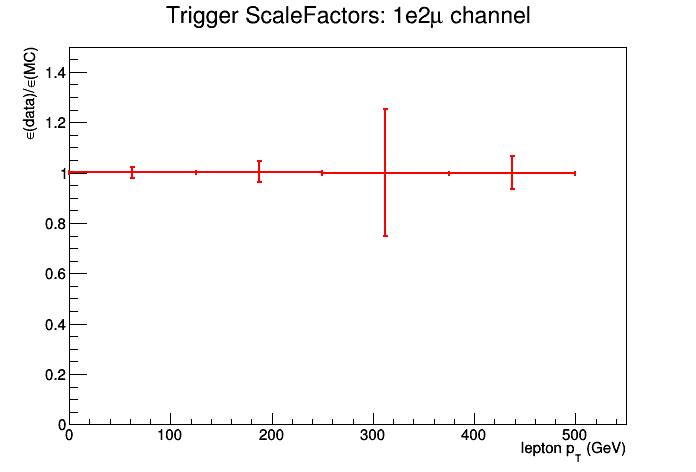
\includegraphics[width=0.48\textwidth]{Appendix/Figures/trigger/Intext/SF_trigger_1e2muhistPt.png}
%	%		\label{image:SF_trigger_1e2muhistPt.png}
%	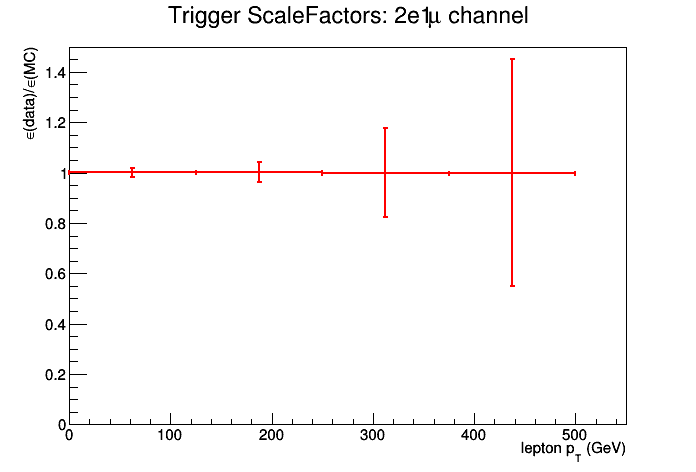
\includegraphics[width=0.48\textwidth]{Appendix/Figures/trigger/Intext/SF_trigger_2e1muhistPt.png}
%	%		\label{image:SF_trigger_2e1muhistPt.png}
%	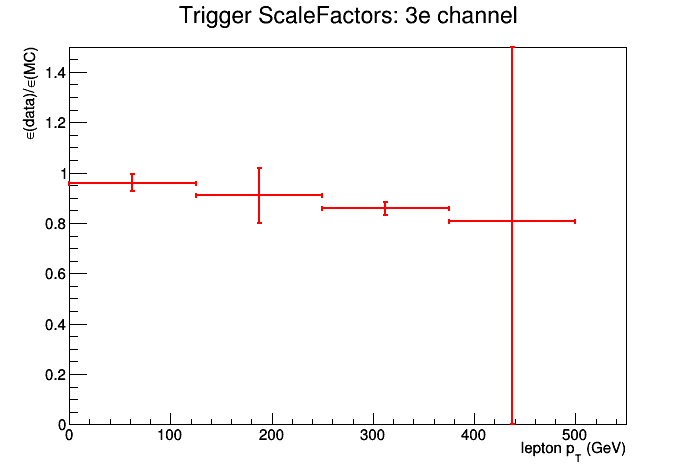
\includegraphics[width=0.48\textwidth]{Appendix/Figures/trigger/Intext/SF_trigger_3ehistPt.png}
%	%		\label{image:SF_trigger_3ehistPt.png}
%	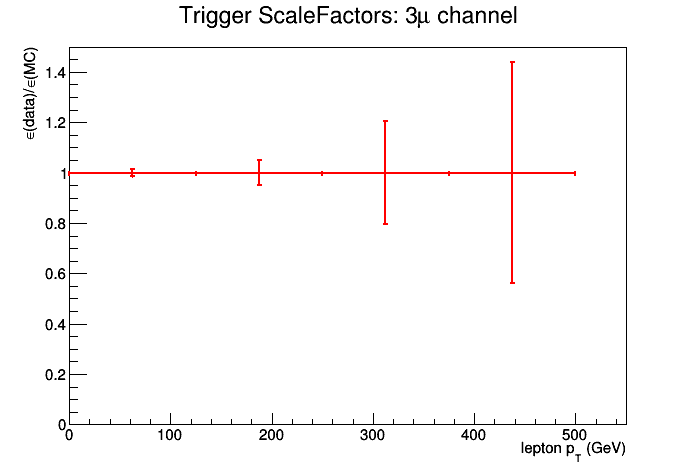
\includegraphics[width=0.48\textwidth]{Appendix/Figures/trigger/Intext/SF_trigger_3muhistPt.png}
%	%		\label{image:SF_trigger_3muhistPt.png}
%	
%	\caption{The trigger scale factors measured as a function of lepton \pt, using the dataset collected by \Etmis\ triggers and \WZ\ simulation, after requiring three leptons and jets selection criteria, in the Z mass window. All corrections to simulation are applied. Left, upper: \emumu\ channel. Right, upper: \eemu\ channel. Left, lower: \eee\ channel. Right, lower: \mumumu\ channel.}
%	\label{image:FigurestriggerIntext}
%\end{figure}
The trigger efficiencies are measured to be nearly 100\% for both simulation and data. The results are dominated by statistics and assigning a large uncertainty to the trigger efficiency based on the dataset collected by \Etmis\ triggers, would be over-conservative. A one percent uncertainty on the trigger selection for the \eemu\ and \mumumu\ final states, and 5\% for the \eee\ and \emumu\ final states is assigned instead, in accordance the \SM\ \tZq\ search~\cite{CMS-PAS-TOP-16-020}. No scale factors will be applied on simulation as they are close to unity. % Control plots are made in the dilepton region to validate all corrections applied to simulation.

\section{Corrections}
\label{sec:corrections}
Mismatches between data and simulation are corrected via the use of scale factors. These are elaborately discussed in \Sec{sec:PhysicsObject}. In this section a short overview of the applied corrections on a dilepton dataset is given. Requiring three leptons would enhance the fraction of \NPL\ backgrounds. These backgrounds are however not well simulated and are determined in a data-driven way. For this reason, the study of the agreement between data and simulation is performed with events selected with the trigger logic and trigger paths described in \Sec{sec:trig}, that contain at least one opposite sign (i.e. not the same electric charge) same flavour lepton pair that has an invariant mass $m_{\mathrm{ll}}$ inside a \PZ\ boson mass window of $|m_{\mathrm{ll}}-\mZ|<7.5~\GeV$, and have jets present. The main contributing process in this selection is the \DY\ process. In the following, the distributions relevant for each correction are shown for all lepton channels. Since events with three leptons are not vetoed from the selection, these will be also entering the collection of the dilepton channels, called ``all channels''. The effect of each correction is shown by either applying all corrections except the one under investigation (``before''), and applying all corrections (``after'').

\subsubsection*{Pileup reweighting}
In data, the number of interactions per bunch crossing (pileup) is calculated with a minimum bias cross section of 69.2 mb. The distribution of the number of simulated pileup events is then reweighted to match the expected number of pileup events in data. Pileup reweighting manifests itself as an altered shape of the number of reconstructed primary vertices as can be seen in \fig{fig:nbvertices}.

\begin{figure}[htbp]
	\centering	
	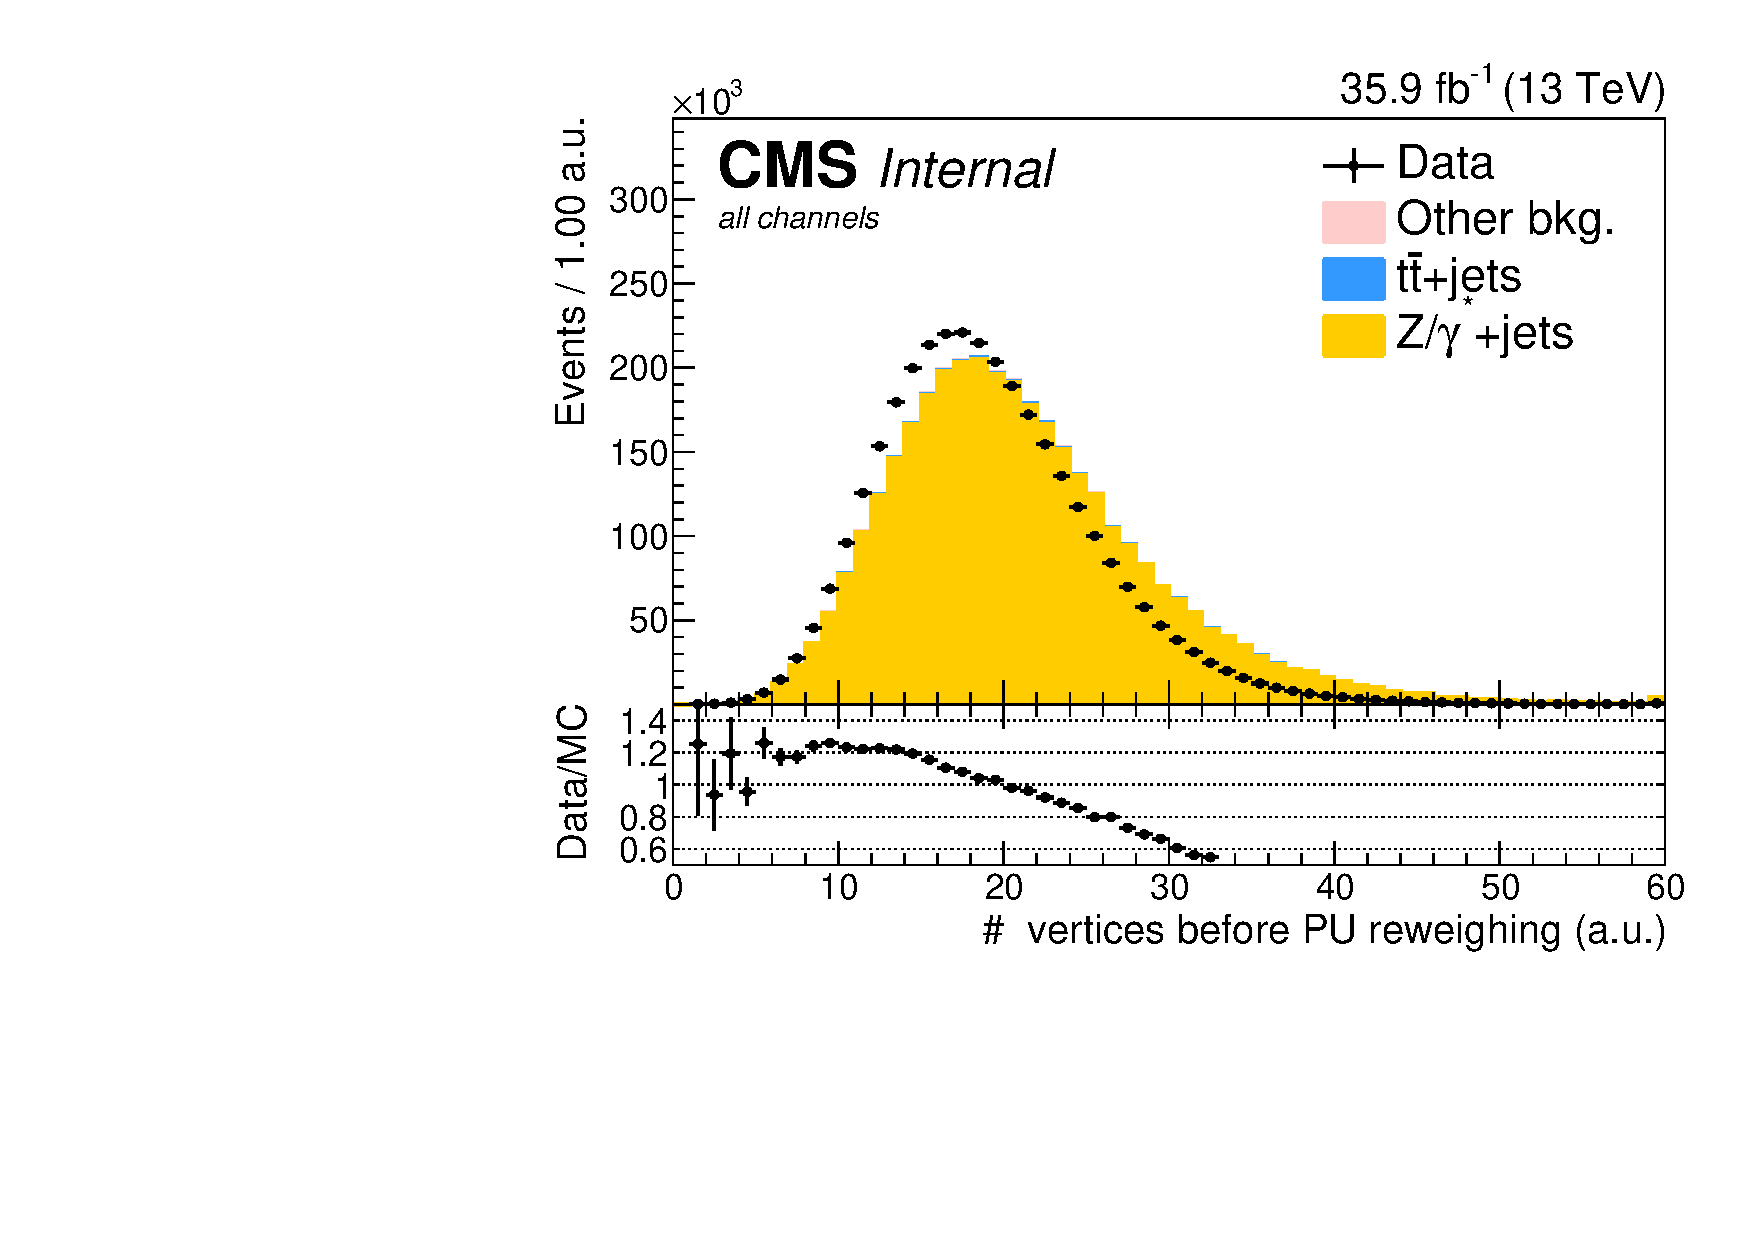
\includegraphics[width=0.49\linewidth]{5_Eventselection/Figures/ReweighingNew/2lepcontrol_dilep_NbOfVertices_bfPU_all_Stack}
	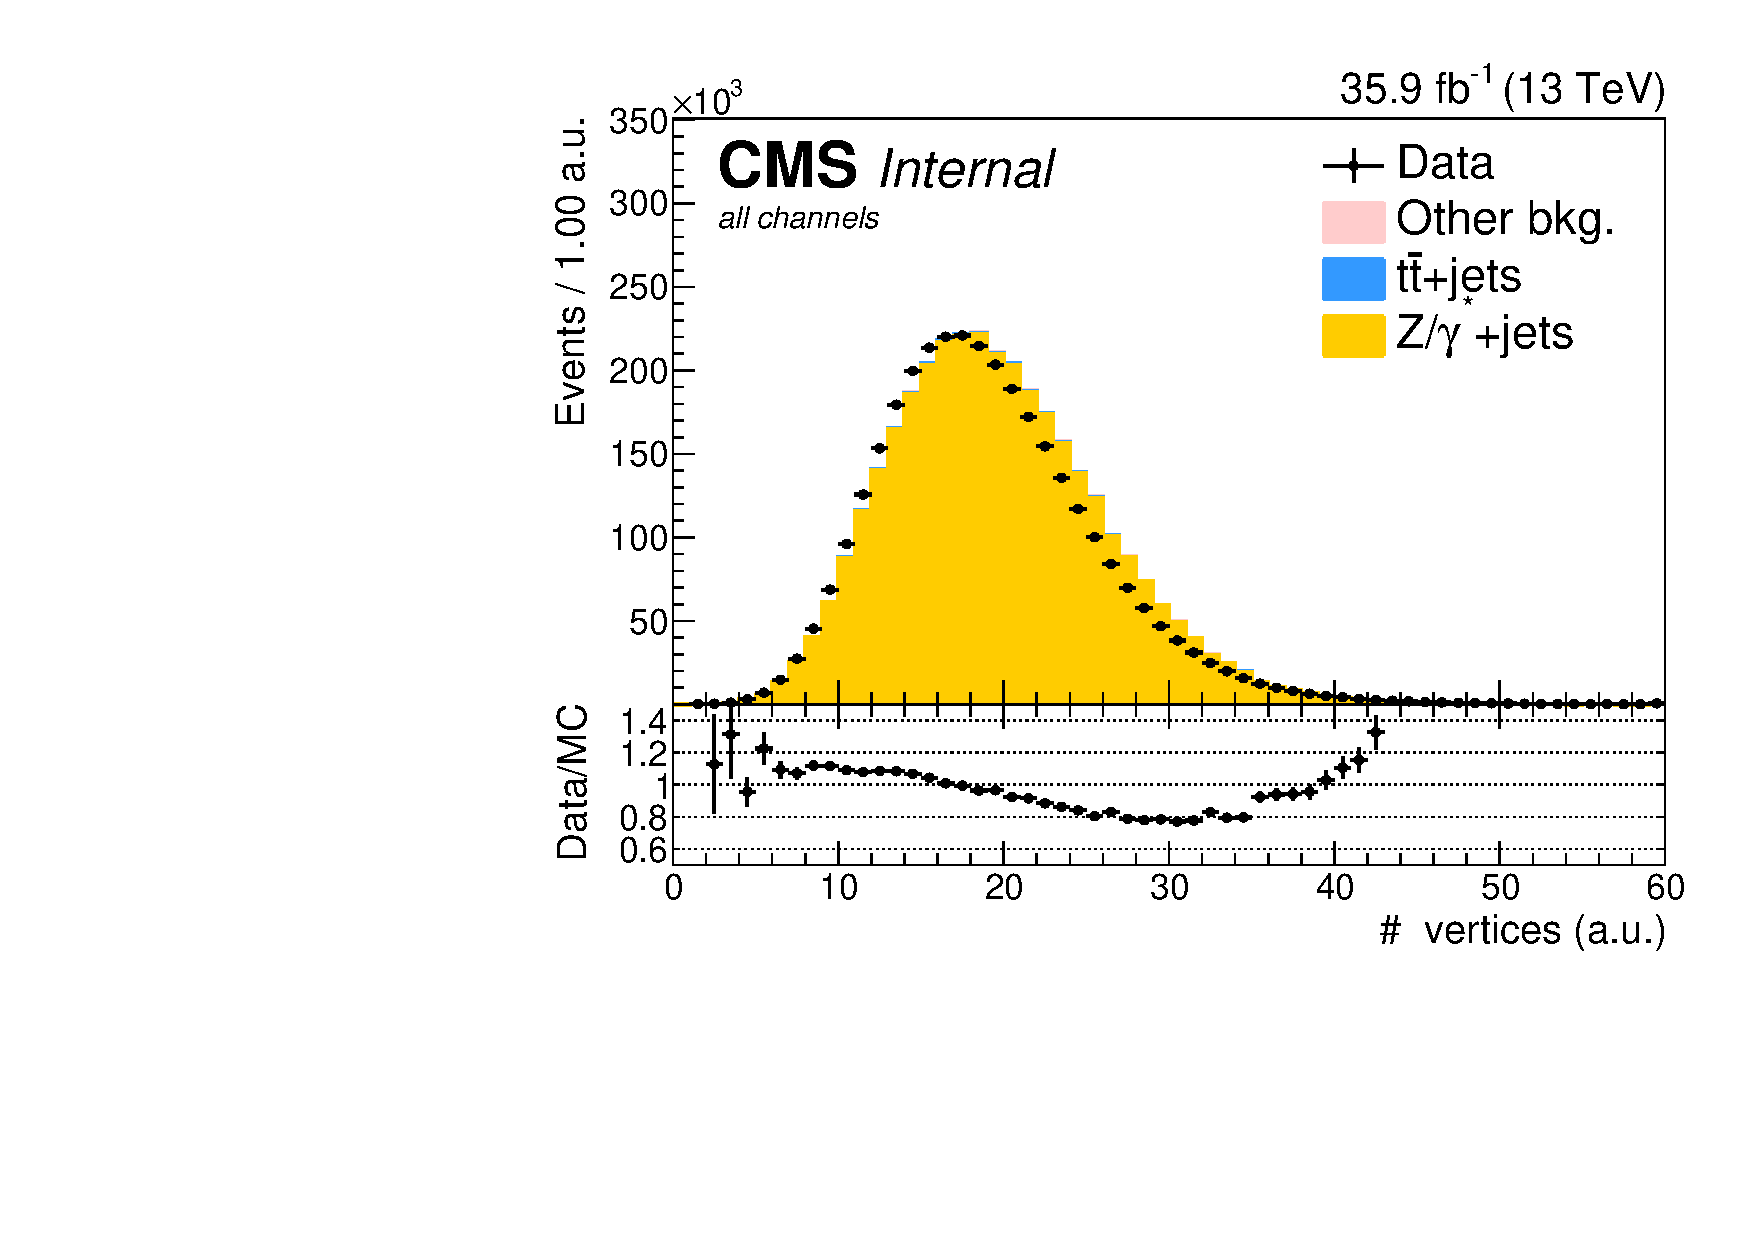
\includegraphics[width=0.49\linewidth]{5_Eventselection/Figures/ReweighingNew/2lepcontrol_dilep_NbOfVertices_all_Stack}
	\caption{Distribution of the number of primary vertices before (left) and after (right) pileup reweighting. Events selected by requiring two leptons in the \PZ\ boson mass window and jets.}
	\label{fig:nbvertices}
\end{figure}

Note that \fig{fig:nbvertices} indicates that even after pileup reweighting, the primary vertex multiplicity is not well described by simulation. This is a known effect, and using  a minimum bias cross section with a slightly lower value is found to better describe the data. However, the scale factors are only provided for the nominal inelastic cross section, and thus this value is used.

%\begin{figure}[htbp]
%	\centering	
%	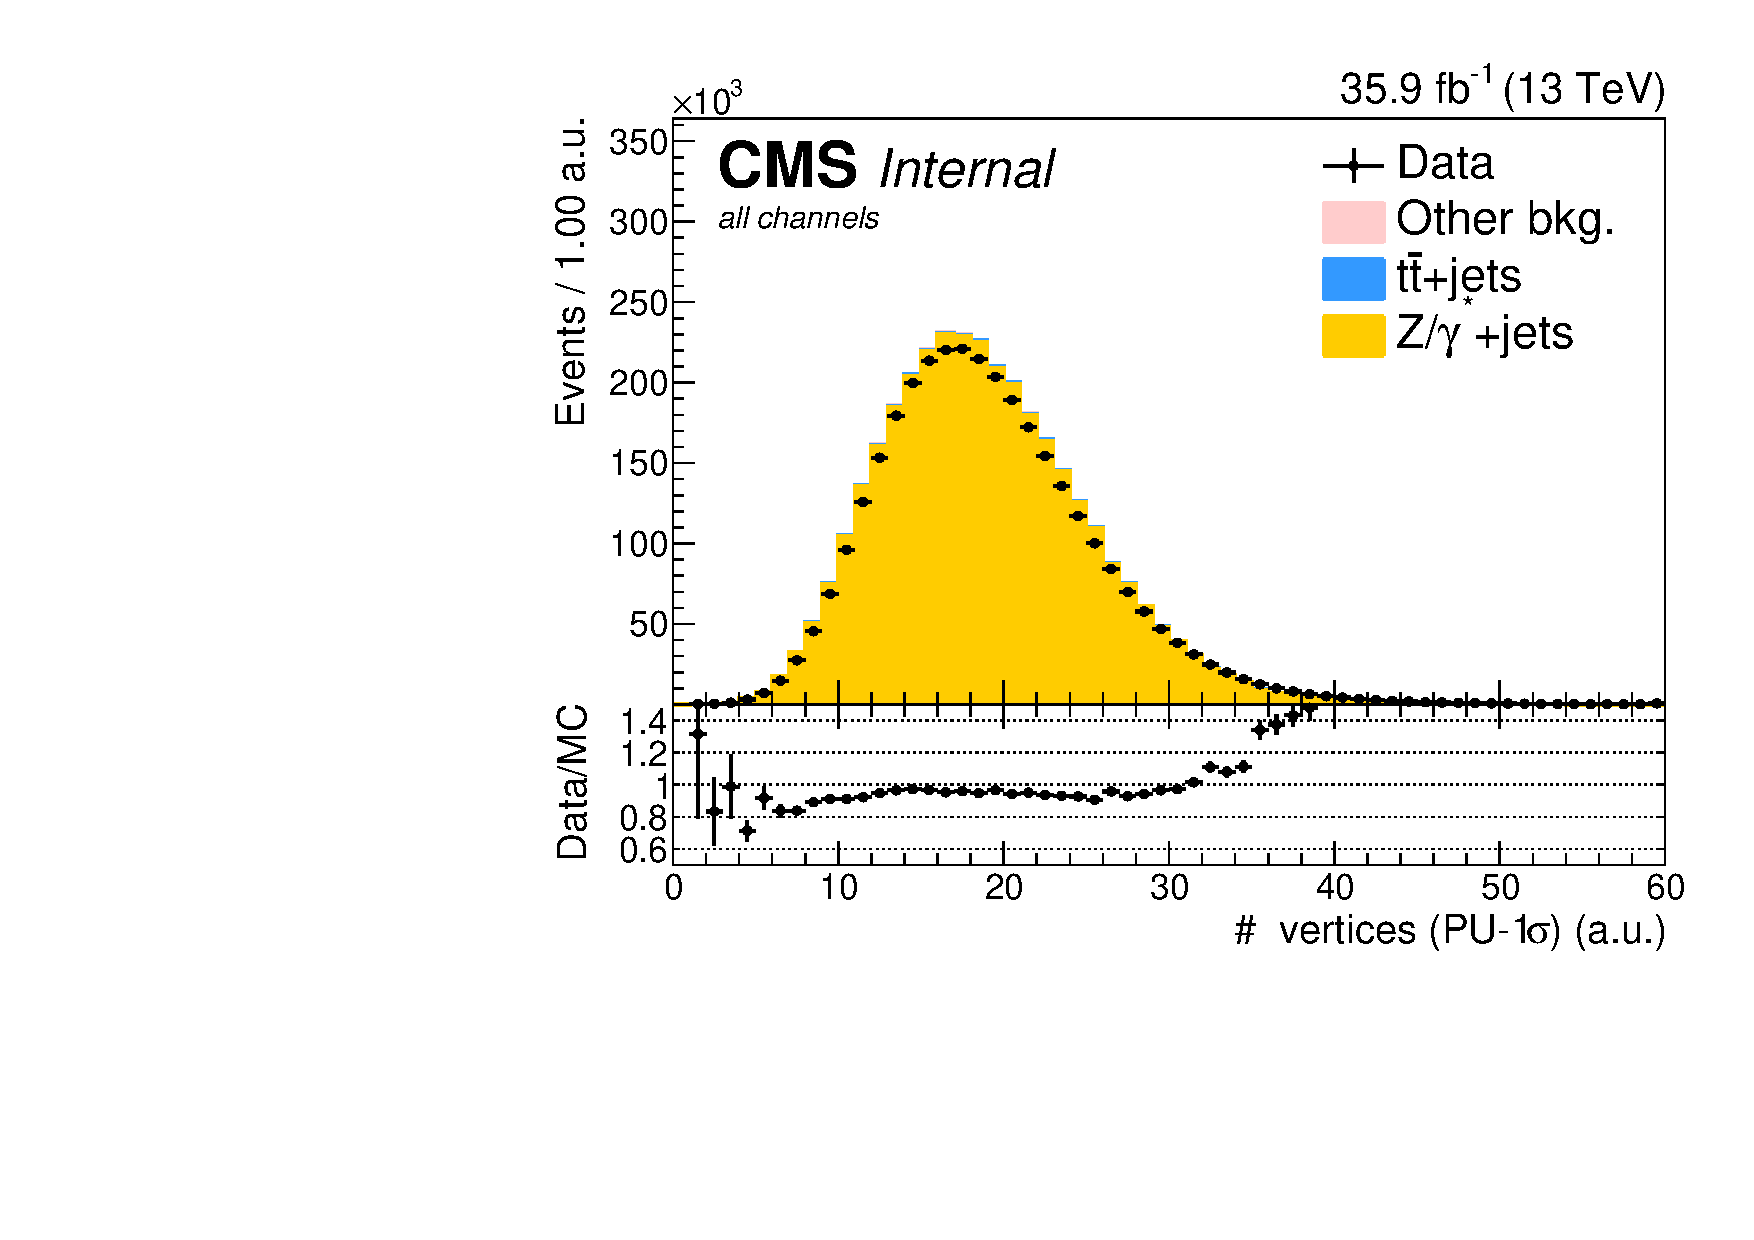
\includegraphics[width=0.49\linewidth]{5_Eventselection/Figures/ReweighingNew/2lepcontrol_dilep_NbOfVertices_1sPU_all_Stack}
%	\caption{Distribution of the number of primary vertices after pileup reweighting, where the scale factor for pileup reweighting is taken at its minus $1\sigma$ uncertainty. Events selected by requiring two leptons in the \PZ\ boson mass window and jets.}
%	\label{fig:nbvertices1s}
%\end{figure}

\subsubsection*{Lepton scale factors}
The efficiency to select leptons is different in simulation ($\epsilon_{\mathrm{MC}}$) compared to the data ($\epsilon_{\mathrm{data}}$). This is corrected for by applying lepton scale factors (SF) to the simulation that are defined as
\begin{equation}
SF = \frac{\epsilon_{\mathrm{data}}}{\epsilon_{\mathrm{MC}}}. 
\end{equation}
These scale factors are measured for the identification, isolation, tracking and trigger efficiencies of the objects as a function of \pt\ and $\eta$ (see \Sec{sec:MuonID} and \Sec{sec:ElectronID}). Multiplying these scale factors for each lepton provides an overall efficiency per event:
\begin{equation}
SF^{\mu}_{\mathrm{global}} = \prod \limits_{\mathrm{i}}^{\# \mu}  SF^{\mu}_{\mathrm{ID}}(\pt,\eta) \: SF^{\mu}_{\mathrm{Iso.}}(\pt,\eta)\: SF^{\mu}_{\mathrm{Trig.}}(\pt,\eta) \:SF^{\mu}_{\mathrm{Track}}(\pt,\eta),
\end{equation}
\begin{equation}
SF^{\mathrm{e}}_{\mathrm{global}} = \prod \limits_{\mathrm{i}}^{\# e}  SF^{\mathrm{e}}_{\mathrm{ID}}(\pt,\eta)\: SF^{\mathrm{e}}_{\mathrm{Iso.}}(\pt,\eta) \: SF^{\mathrm{e}}_{\mathrm{Trig.}}(\pt,\eta) \: SF^{\mathrm{e}}_{\mathrm{Track}}(\pt,\eta) .
\end{equation}
The effect of the scale factors can be found in \fig{fig:muSF} for the muons and \fig{fig:elSF} for the electrons. The trigger efficiencies are estimated in \Sec{sec:triggereff}.

\begin{figure}[htbp]
	\centering
	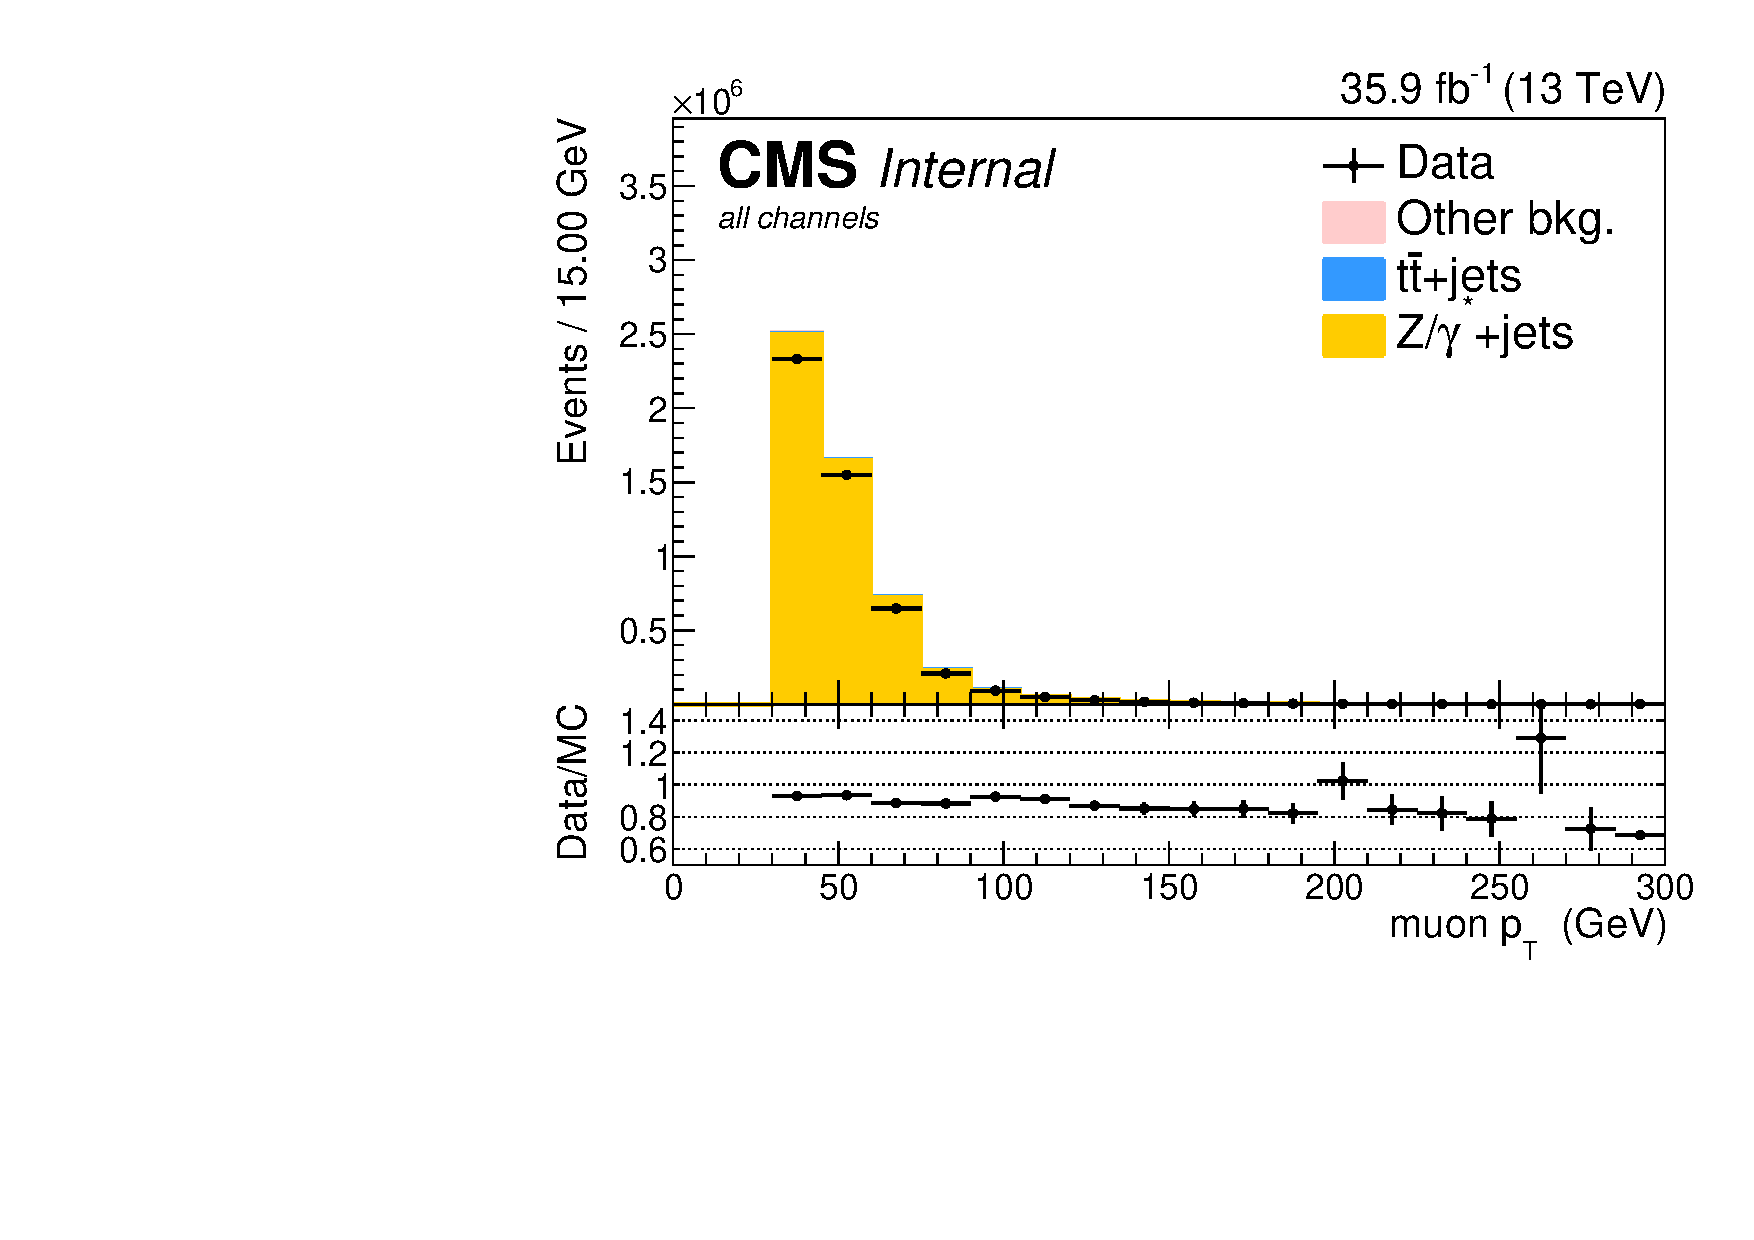
\includegraphics[width=0.49\linewidth]{5_Eventselection/Figures/Reweighing/2lepcontrol_dilep_MuPt_all_Stackbefore}
	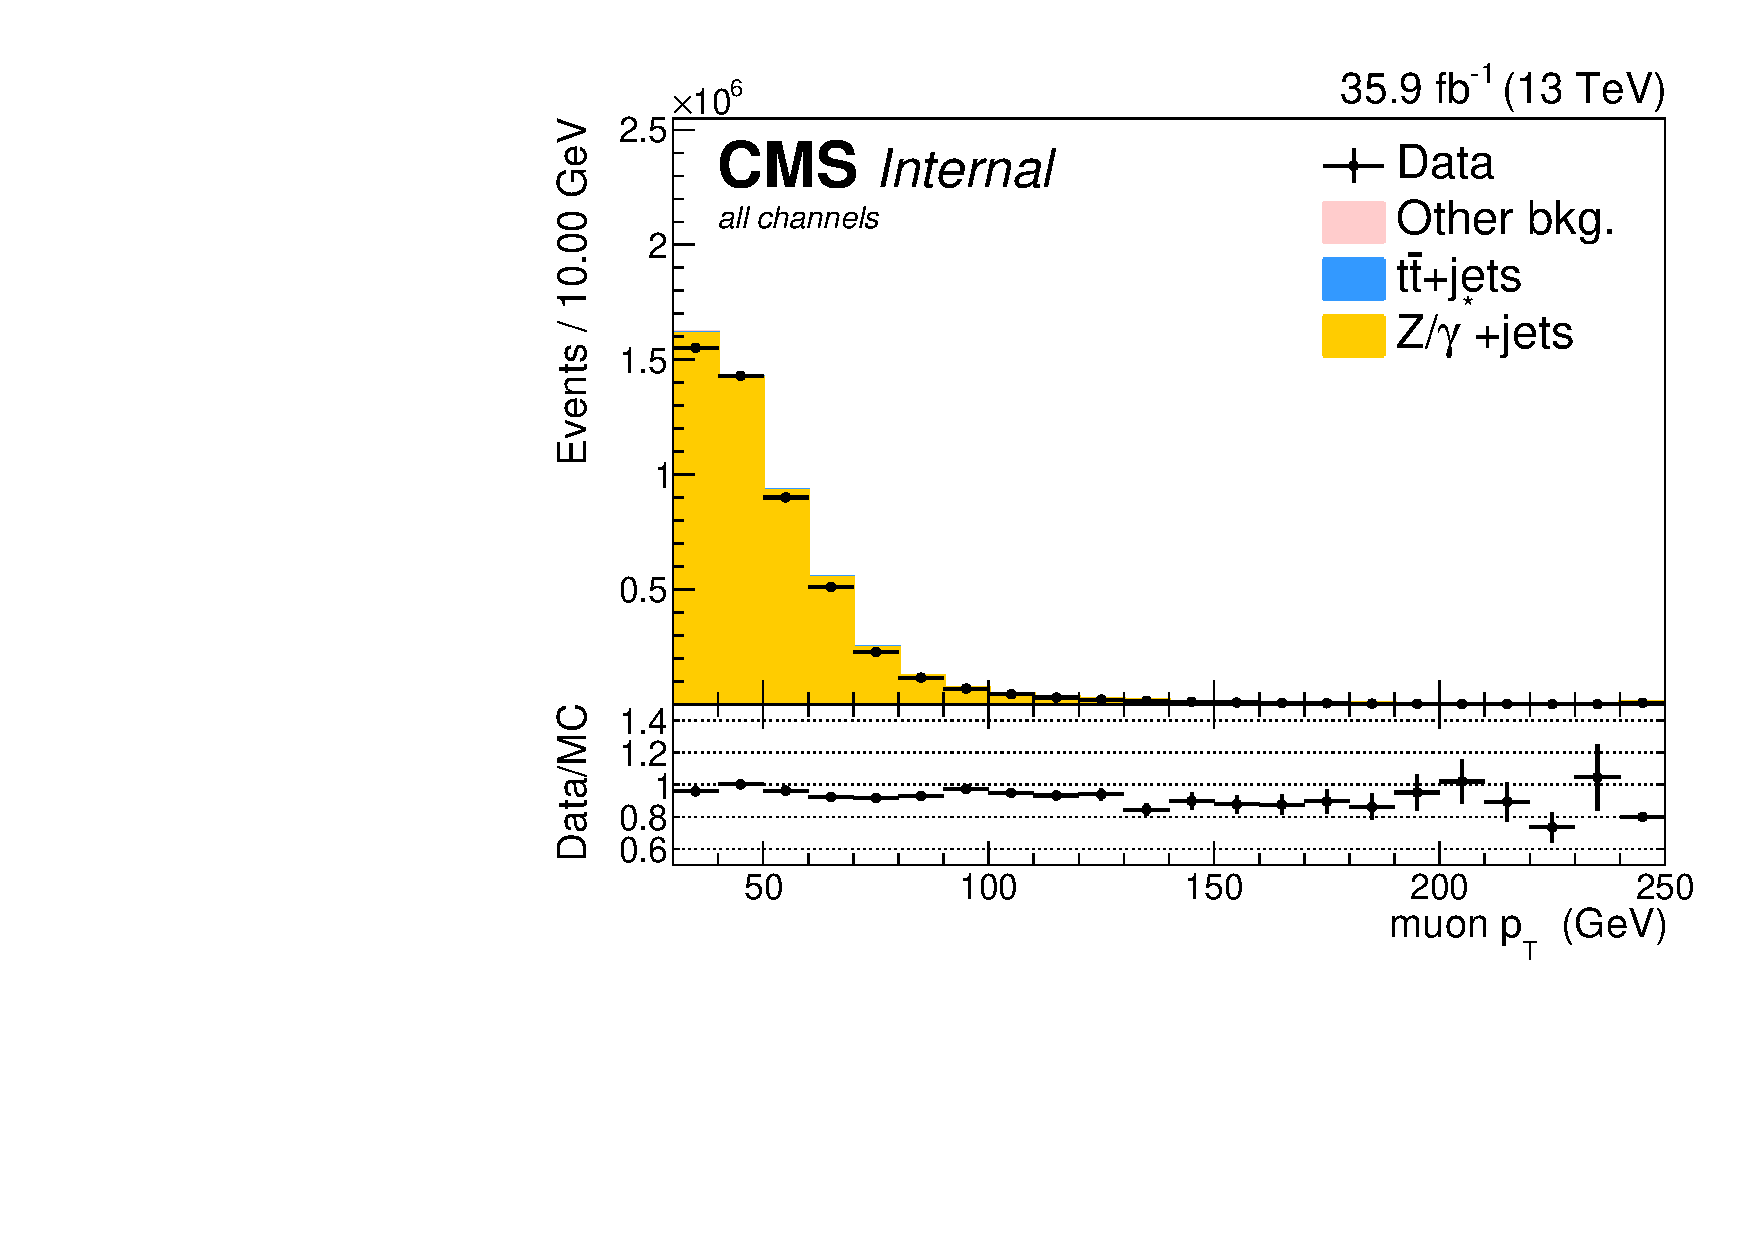
\includegraphics[width=0.49\linewidth]{5_Eventselection/Figures/Reweighing/2lepcontrol_dilep_MuPt_all_Stack}
	\caption{Distribution of the \pt\ of the muons before (left) and after (right) muon scale factors.  Events selected by requiring two leptons in the \PZ\ boson mass window and jets. All other corrections are applied.}
	\label{fig:muSF}
\end{figure}
\begin{figure}[htbp]
	\centering
	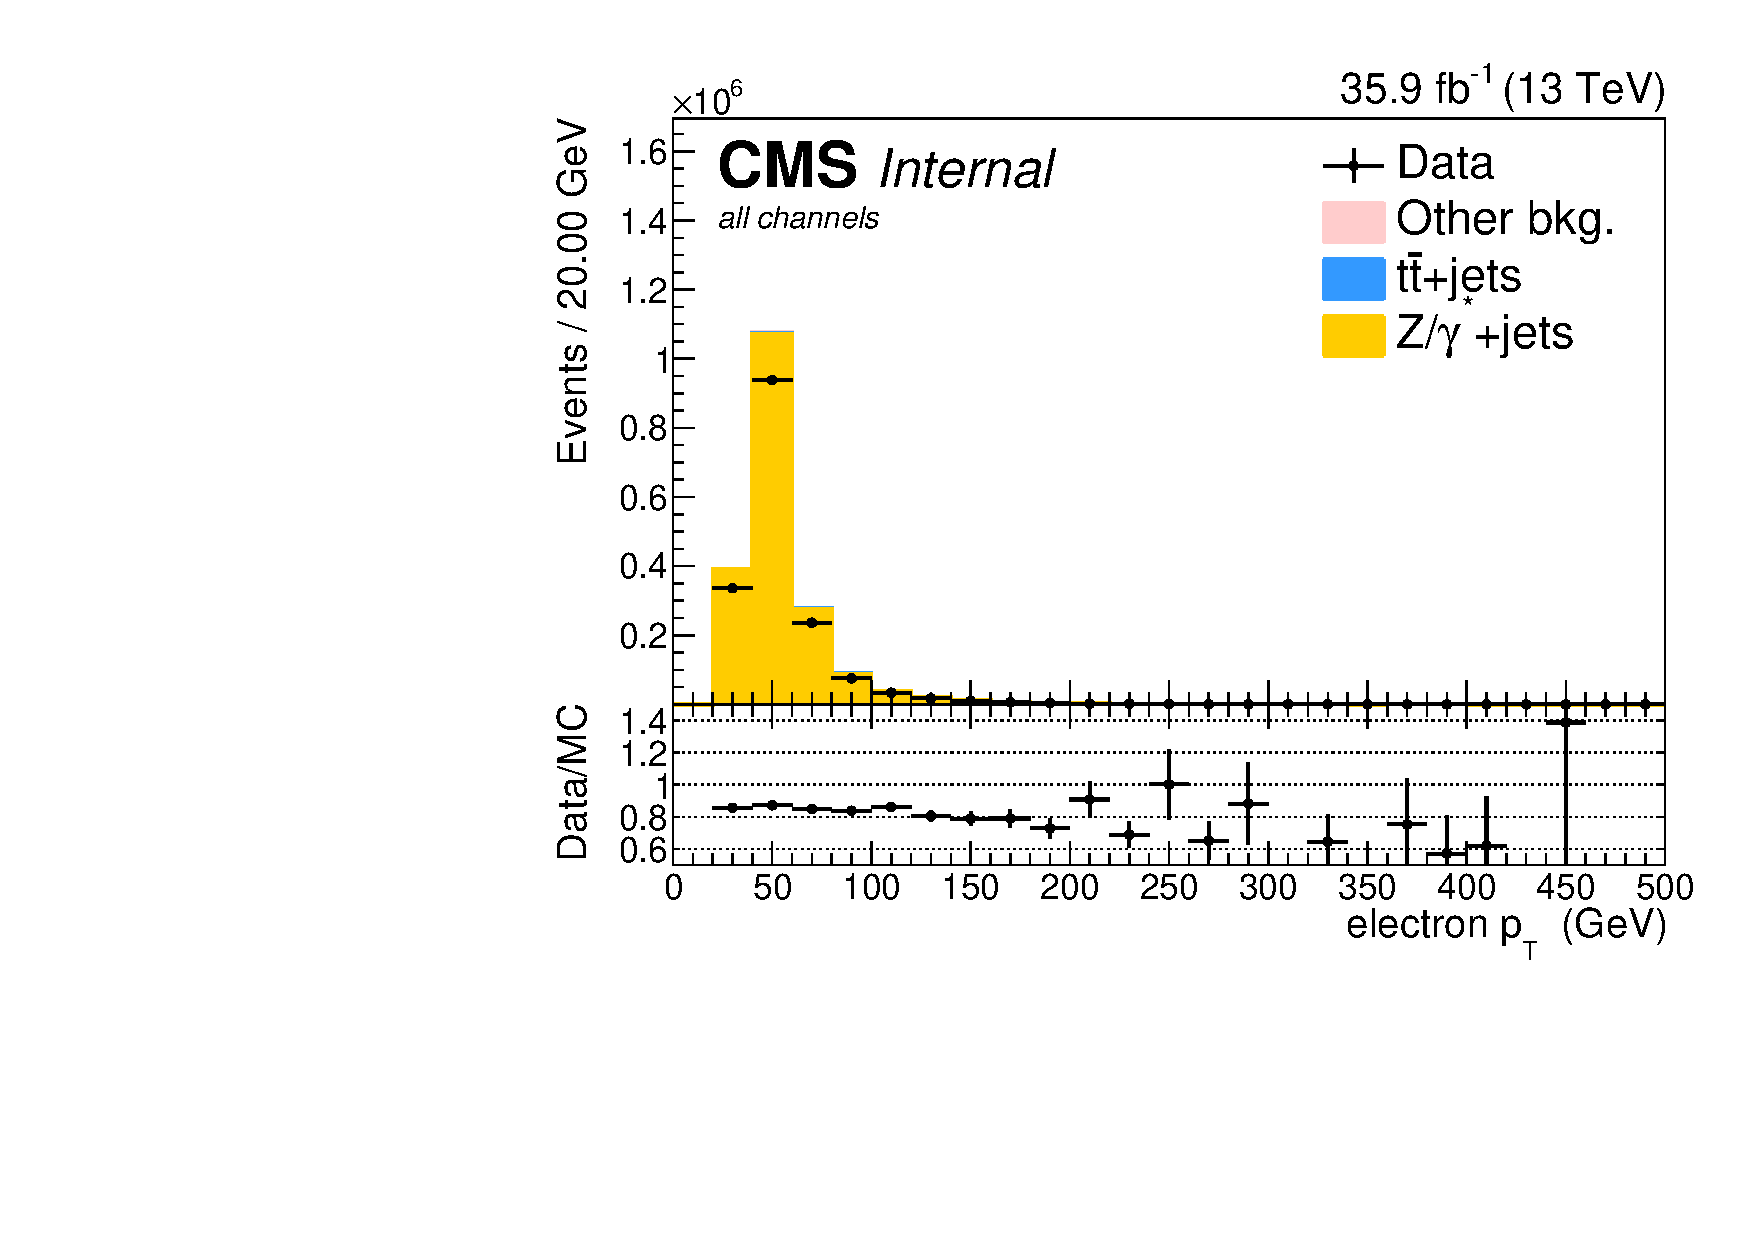
\includegraphics[width=0.49\linewidth]{5_Eventselection/Figures/Reweighing/2lepcontrol_dilep_ElPt_all_Stackbefore}
	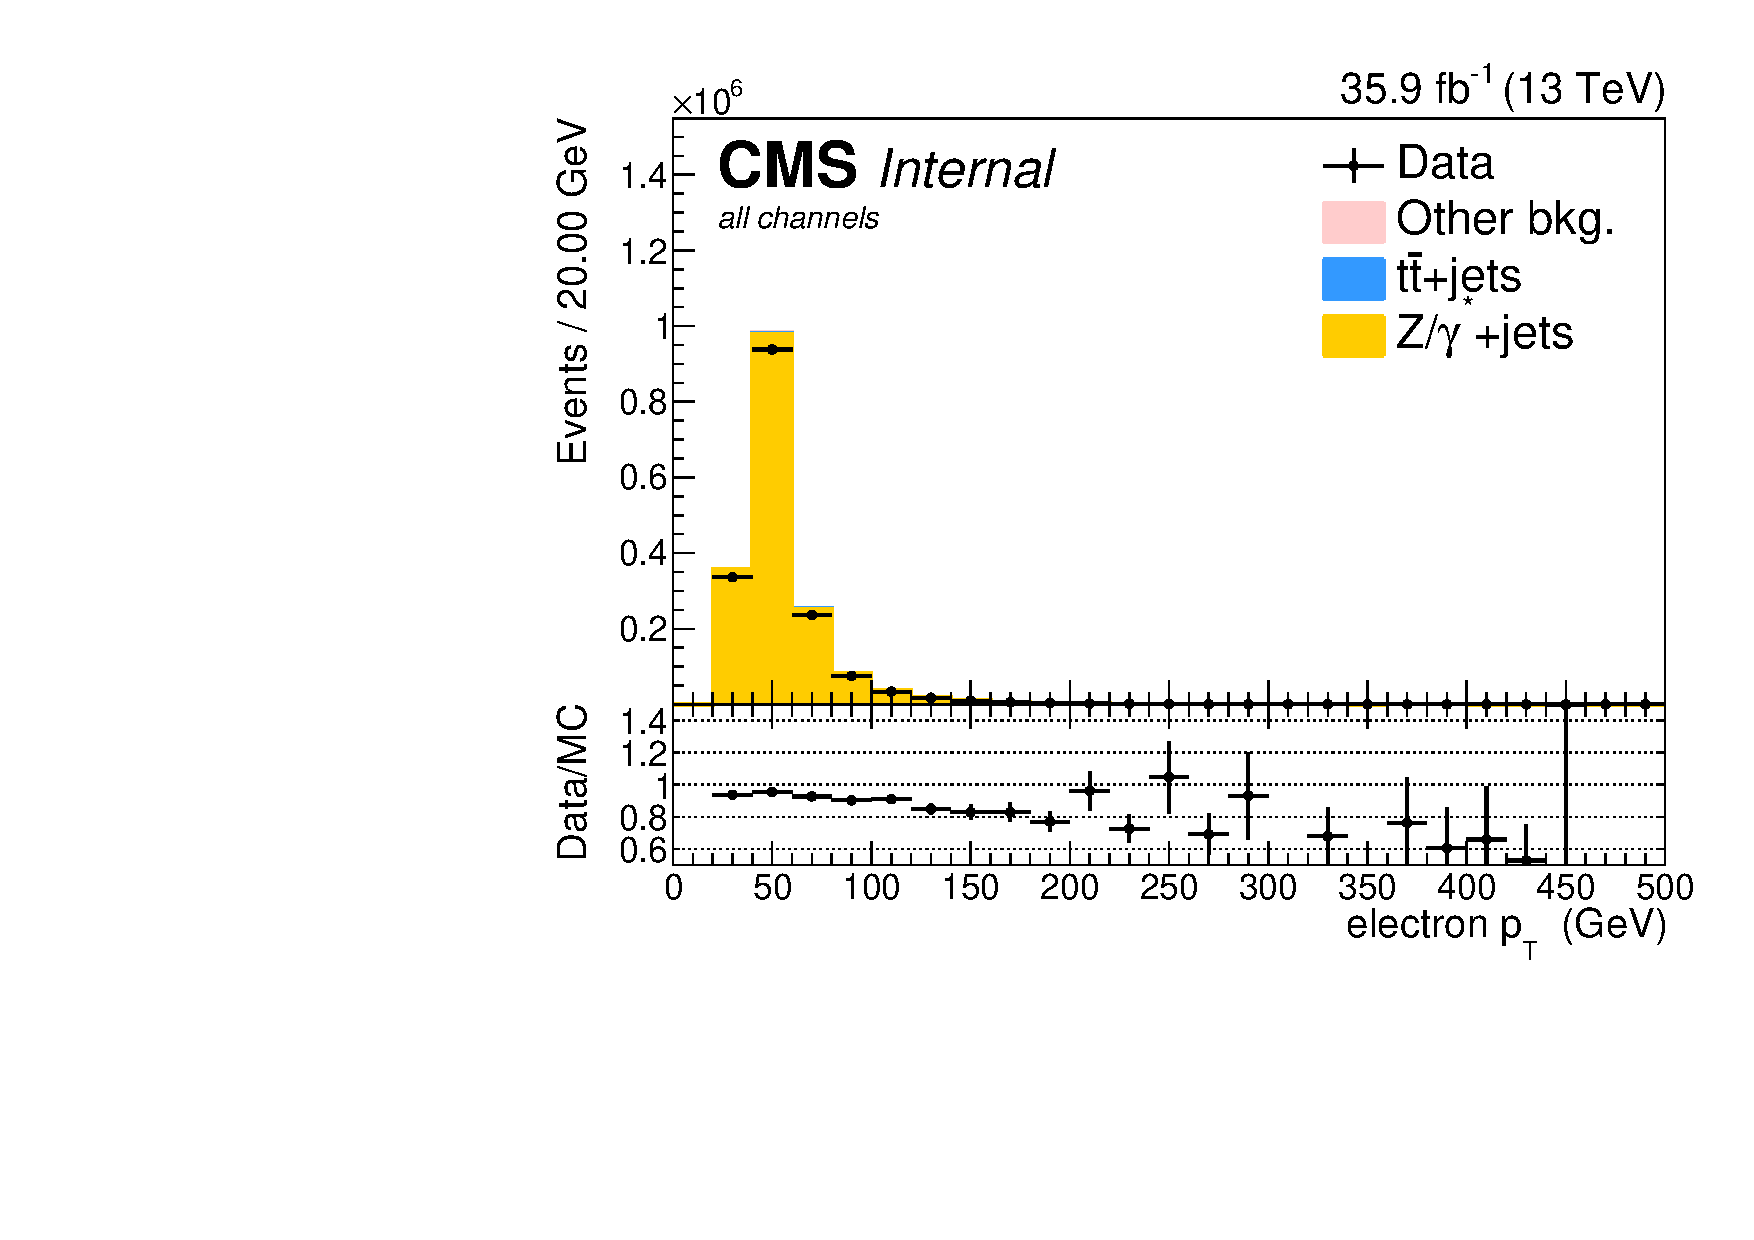
\includegraphics[width=0.49\linewidth]{5_Eventselection/Figures/Reweighing/2lepcontrol_dilep_ElPt_all_Stack}
	\caption{Distribution of the \pt\ of the electrons before (left) and after (right) electron scale factors.  Events selected by requiring two leptons in the \PZ\ boson mass window and jets. All other corrections are applied.}
	\label{fig:elSF}
\end{figure}

Additionally, corrections are determined from $\PZ\rightarrow \Pe \Pe$ events for the energy resolution of the leptons. For the electrons, energy smearing and regression is applied \cite{smearing}. The energy regression uses the detector information to correct the electron energy in order to have the best energy resolution and corrects for material effects in the ECAL, improving the performance. The energy scale and smearing corrects the simulation energies to have identical energy resolution in simulation and data. For the muons, the \pt\ is corrected using the Rochester method \cite{roch,roch2}. This correction is determined from $\PZ\rightarrow \Pmu \Pmu$ events and removes the bias of the muon \pt\ from any detector misalignment or any possible error of the magnetic field. The effect of the Rochester correction can be found in \fig{fig:roch}.
%https://indico.cern.ch/event/658669/contributions/2746905/attachments/1558017/2451133/top_egm.pdf
\begin{figure}[htbp]
	\centering	
	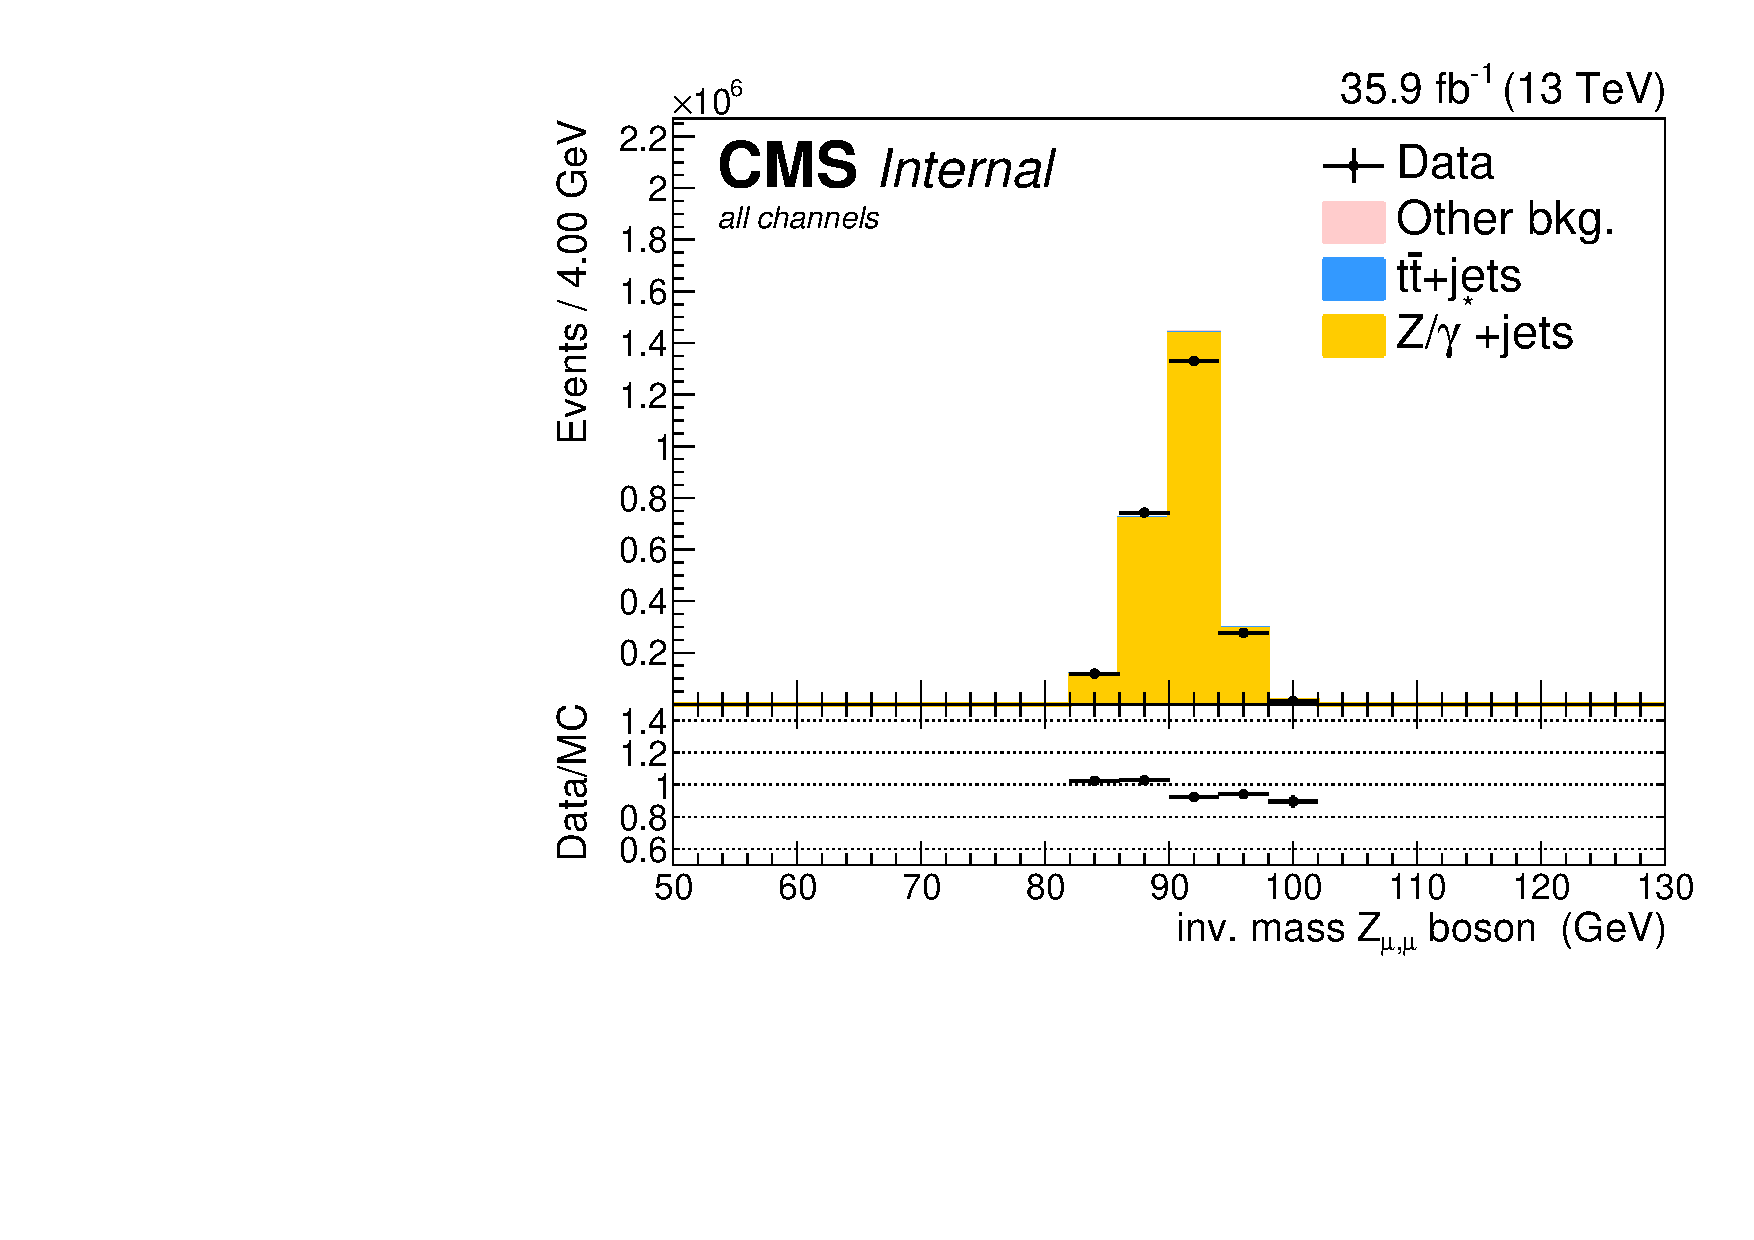
\includegraphics[width=0.49\linewidth]{5_Eventselection/Figures/Reweighing/2lepcontrol_dilep_ZbosonMassMu_all_Stackbefore}
	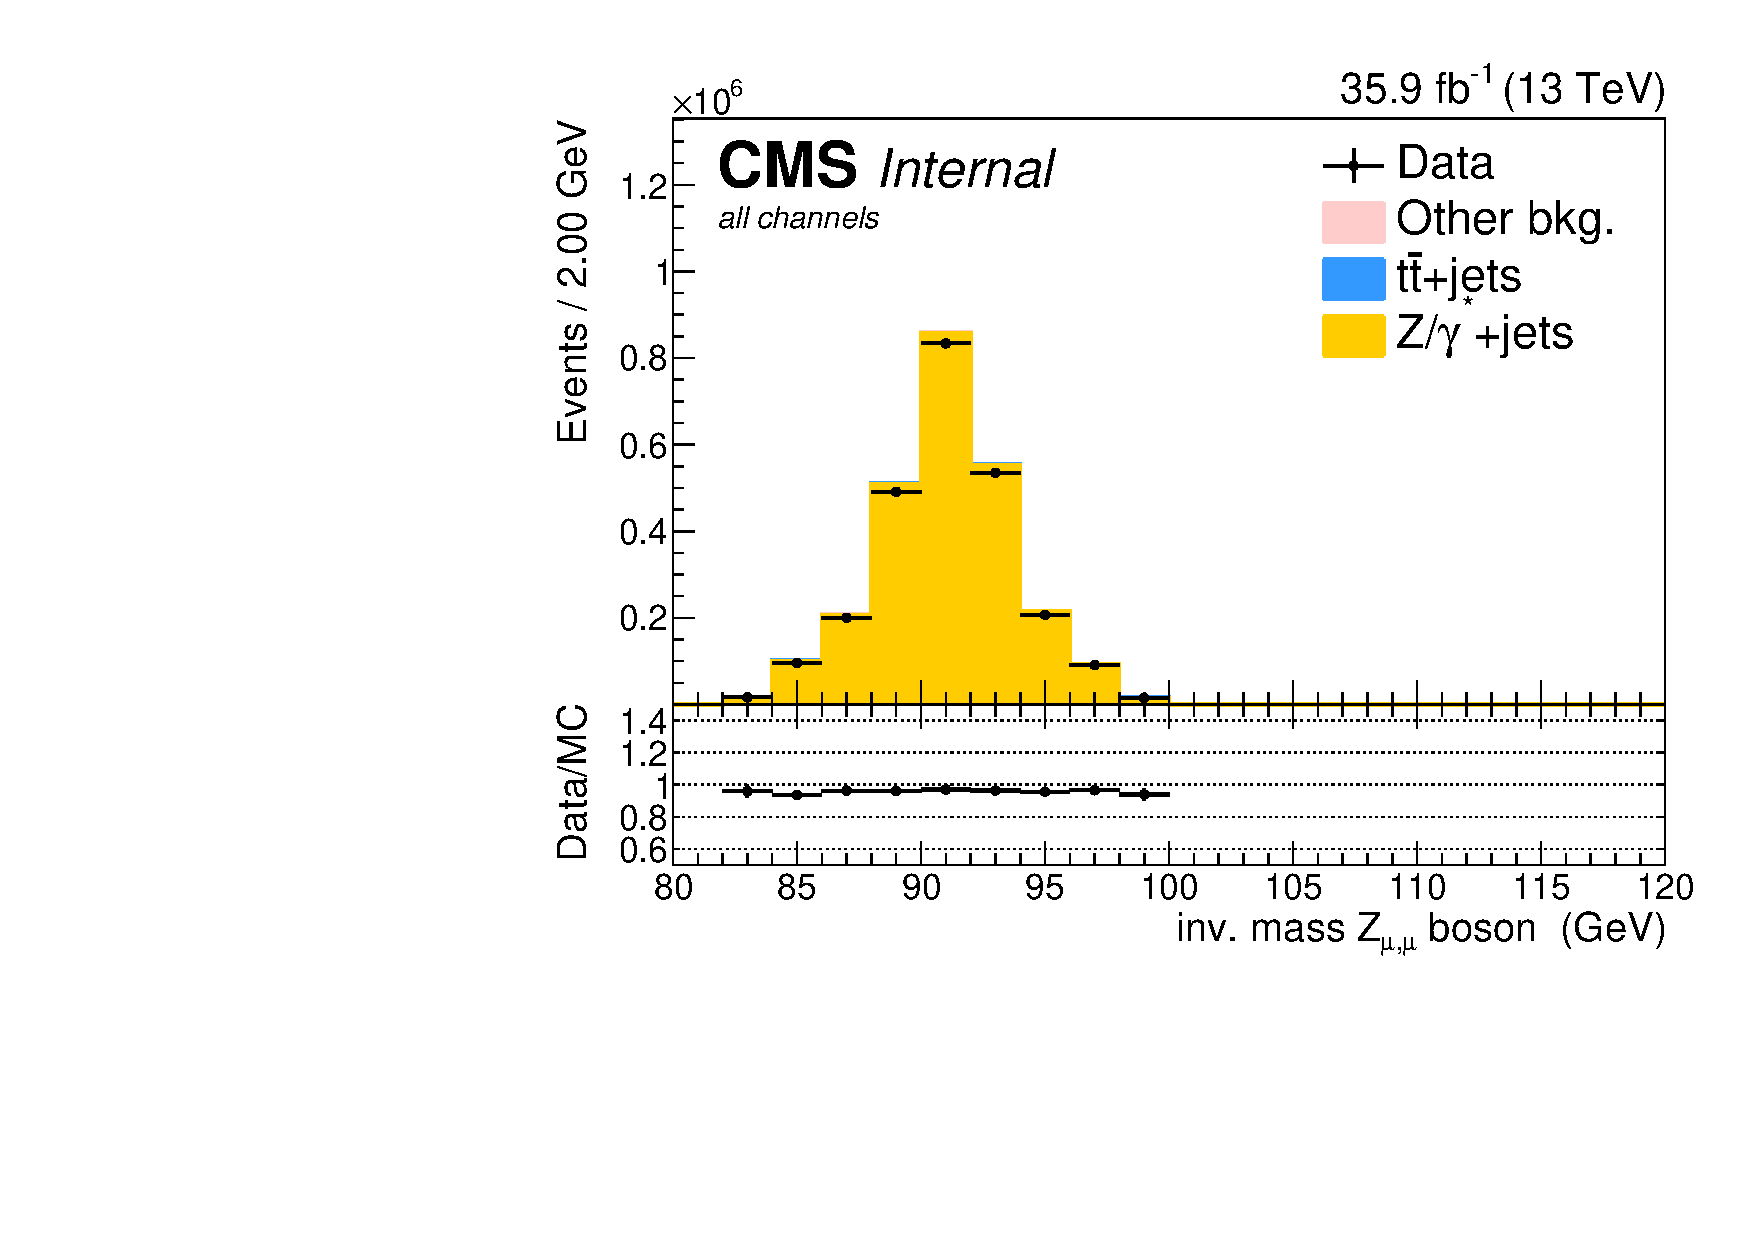
\includegraphics[width=0.49\linewidth]{5_Eventselection/Figures/Reweighing/2lepcontrol_dilep_ZbosonMassMu_all_Stack}
	
	\caption{Distribution of the mass of the \PZ\ boson from muons before (left) and after (right) the Rochester correction.   Events selected by requiring two leptons in the \PZ\ boson mass window and jets. All other corrections are applied.}
	\label{fig:roch}
\end{figure}

\subsubsection*{CSVv2 shape correction}
In order to make the distribution of the CSVv2 b-tagging discriminant in simulation agree with data,  jet-by-jet based scale factors are applied. These scale factors are a function of the \pt, $\eta$ and flavour of the jet as discussed in \Sec{sec:BJetID}.  The effect of these scale factors on the distribution of the CSVv2 discriminant of all jets can be found in \fig{fig:bSF}.


\begin{figure}[htbp]
	\centering
	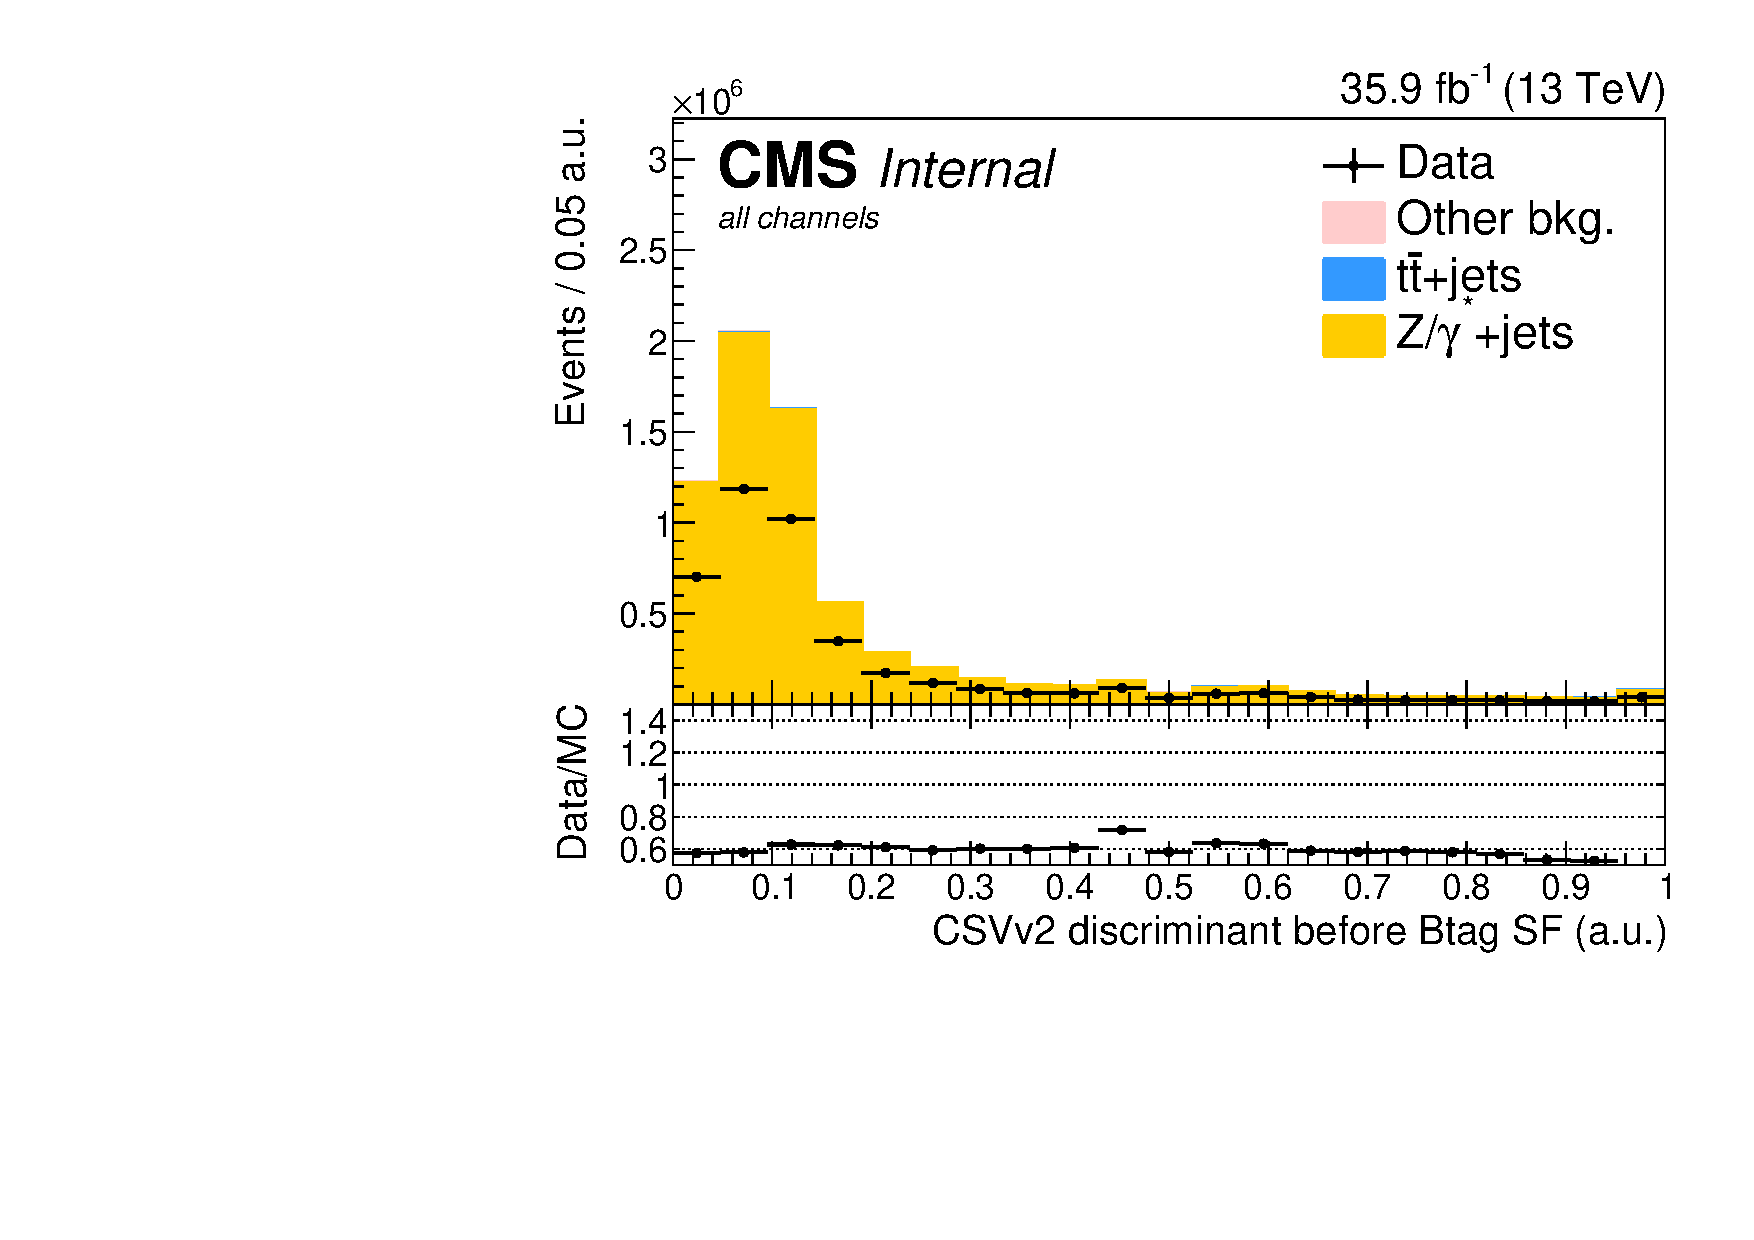
\includegraphics[width=0.49\linewidth]{5_Eventselection/Figures/ReweighingNew/2lepcontrol_dilep_bdisc_bfBT_all_Stack}
	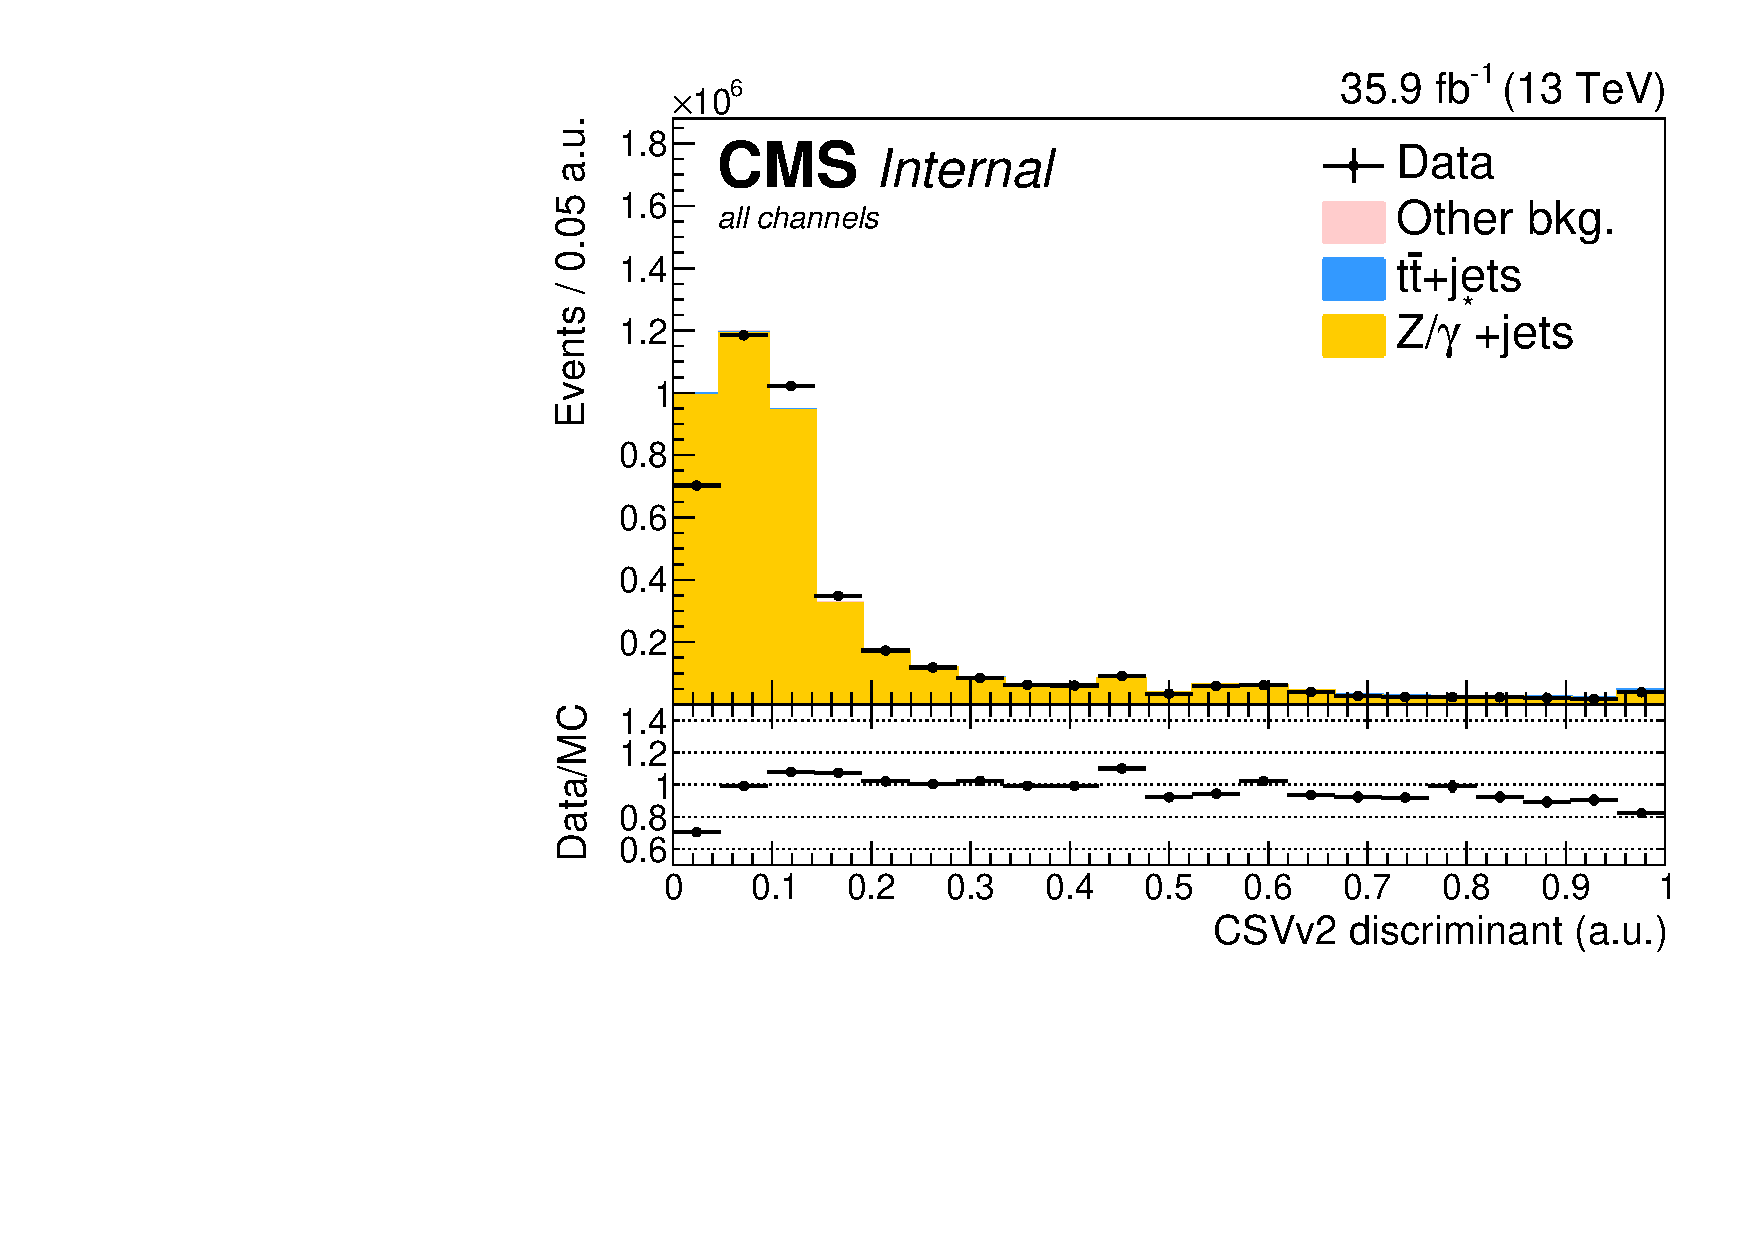
\includegraphics[width=0.49\linewidth]{5_Eventselection/Figures/ReweighingNew/2lepcontrol_dilep_bdisc_all_Stack}	
	\caption{Distribution of the CSVv2 discriminant of the jets before (left) and after (right) b-tag scale factors.  Events selected by requiring two leptons in the \PZ\ boson mass window and jets. All other corrections are applied.}
	\label{fig:bSF}
\end{figure}

\subsubsection*{Jet energy}
\label{sec:jer}
The jet energy in data and simulation is corrected by the measured energy response of the detector. This provides $p_T$- and $\eta$-dependent scale factors and are directly taken from the frontier condition database as discussed in \Sec{sec:JetID}. 
%Additionally, the jet \pt\ resolution is corrected by the scaling method described in \cite{jetsmear}, where the jet \pt\ is rescaled by
%\begin{equation}
%c_{\mathrm{JER}} = 1 + (s_{\mathrm{JER}}-1)\frac{\pt -\pt^{ptcl}}{\pt}.
%\end{equation}
%With \pt\ the reconstructed transverse momentum, \pt$^{ptcl}$ the transverse momentum of the corresponding jet clustered from generator level particles, and $s_{\mathrm{JER}}$ the resolution scale factor. The resolution scale factor is measured in $\eta$ bins and given in Table \ref{tab:JER}. 
The effect of the jet energy corrections on the distribution of the \pt\ of all jets can be found in \fig{fig:jesSF} and \fig{fig:jerSF}.

\begin{figure}[htbp]
	\centering
	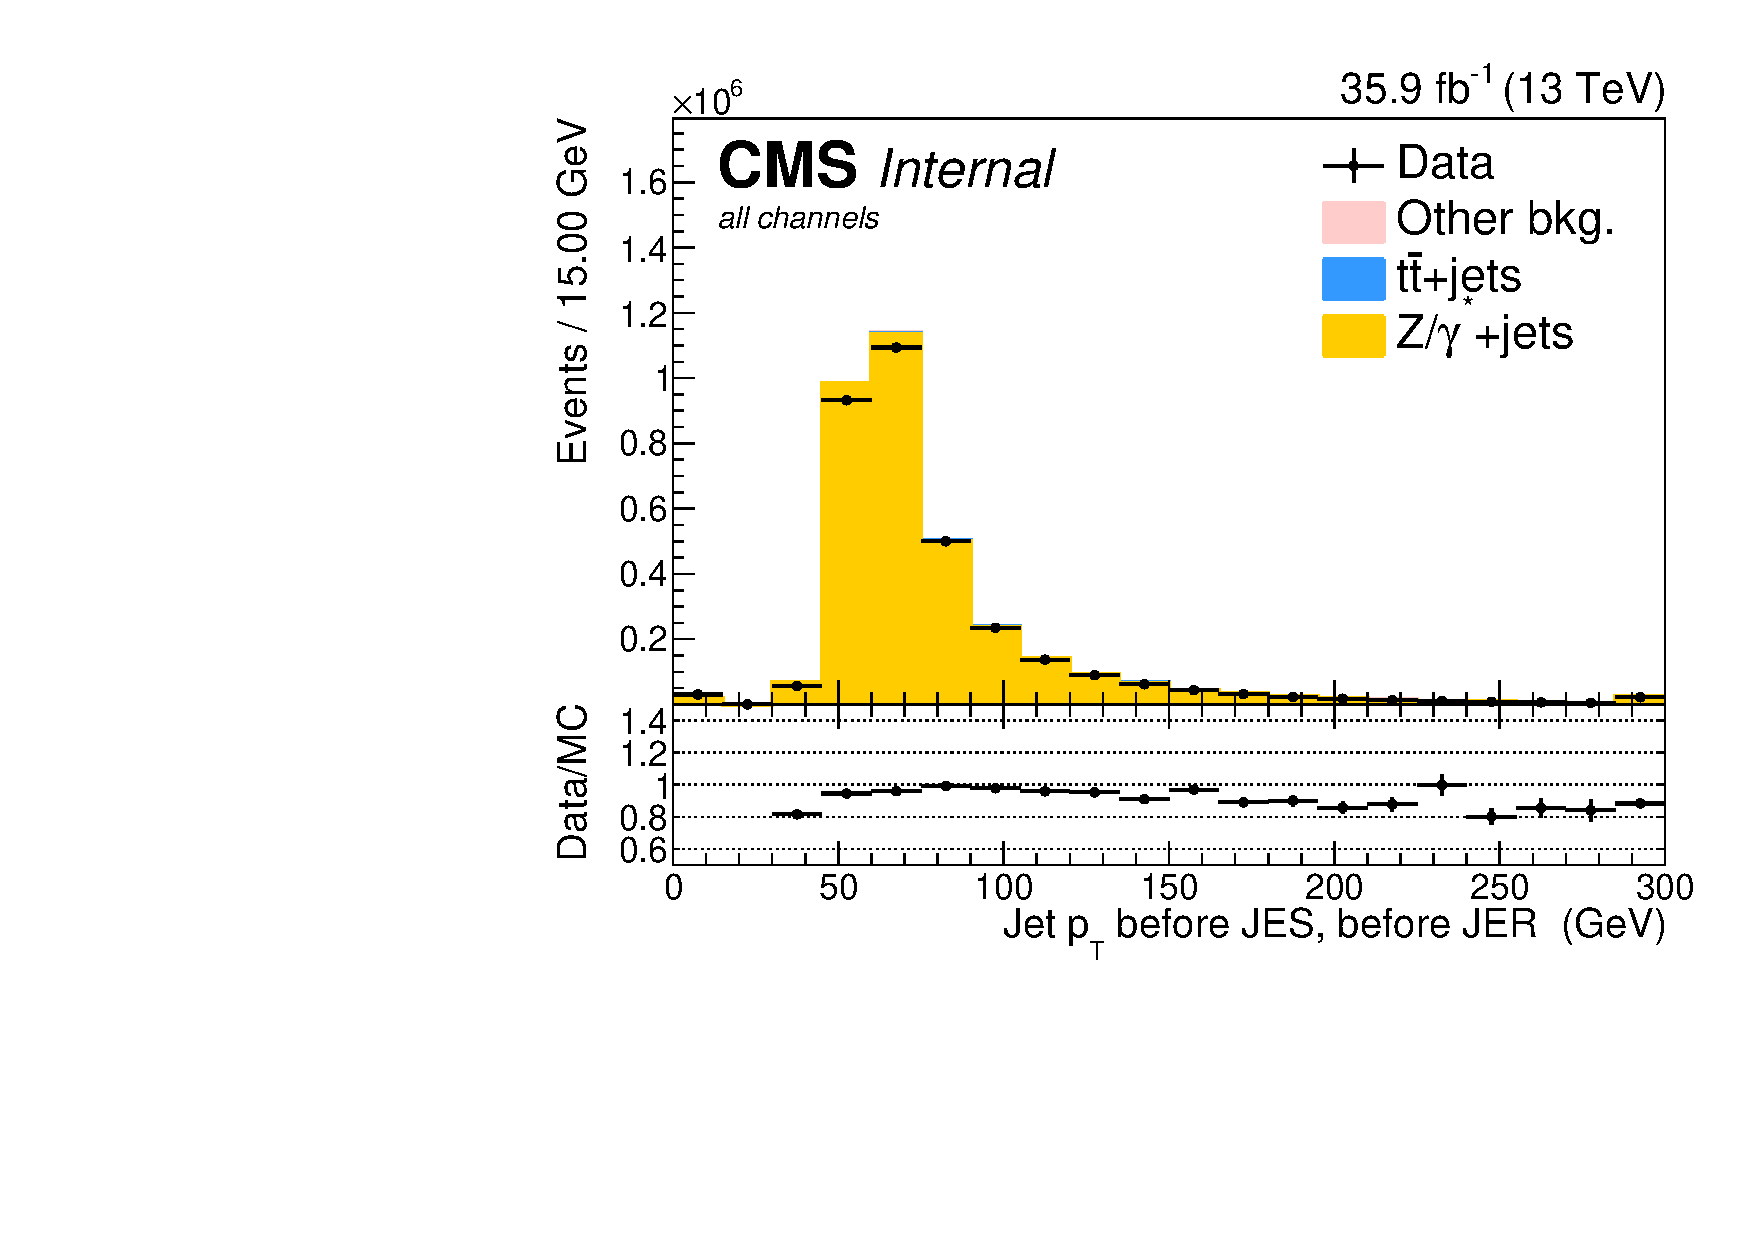
\includegraphics[width=0.49\linewidth]{5_Eventselection/Figures/Reweighing/2lepcontrol_dilep_JetPt_bfJES_all_Stack}
	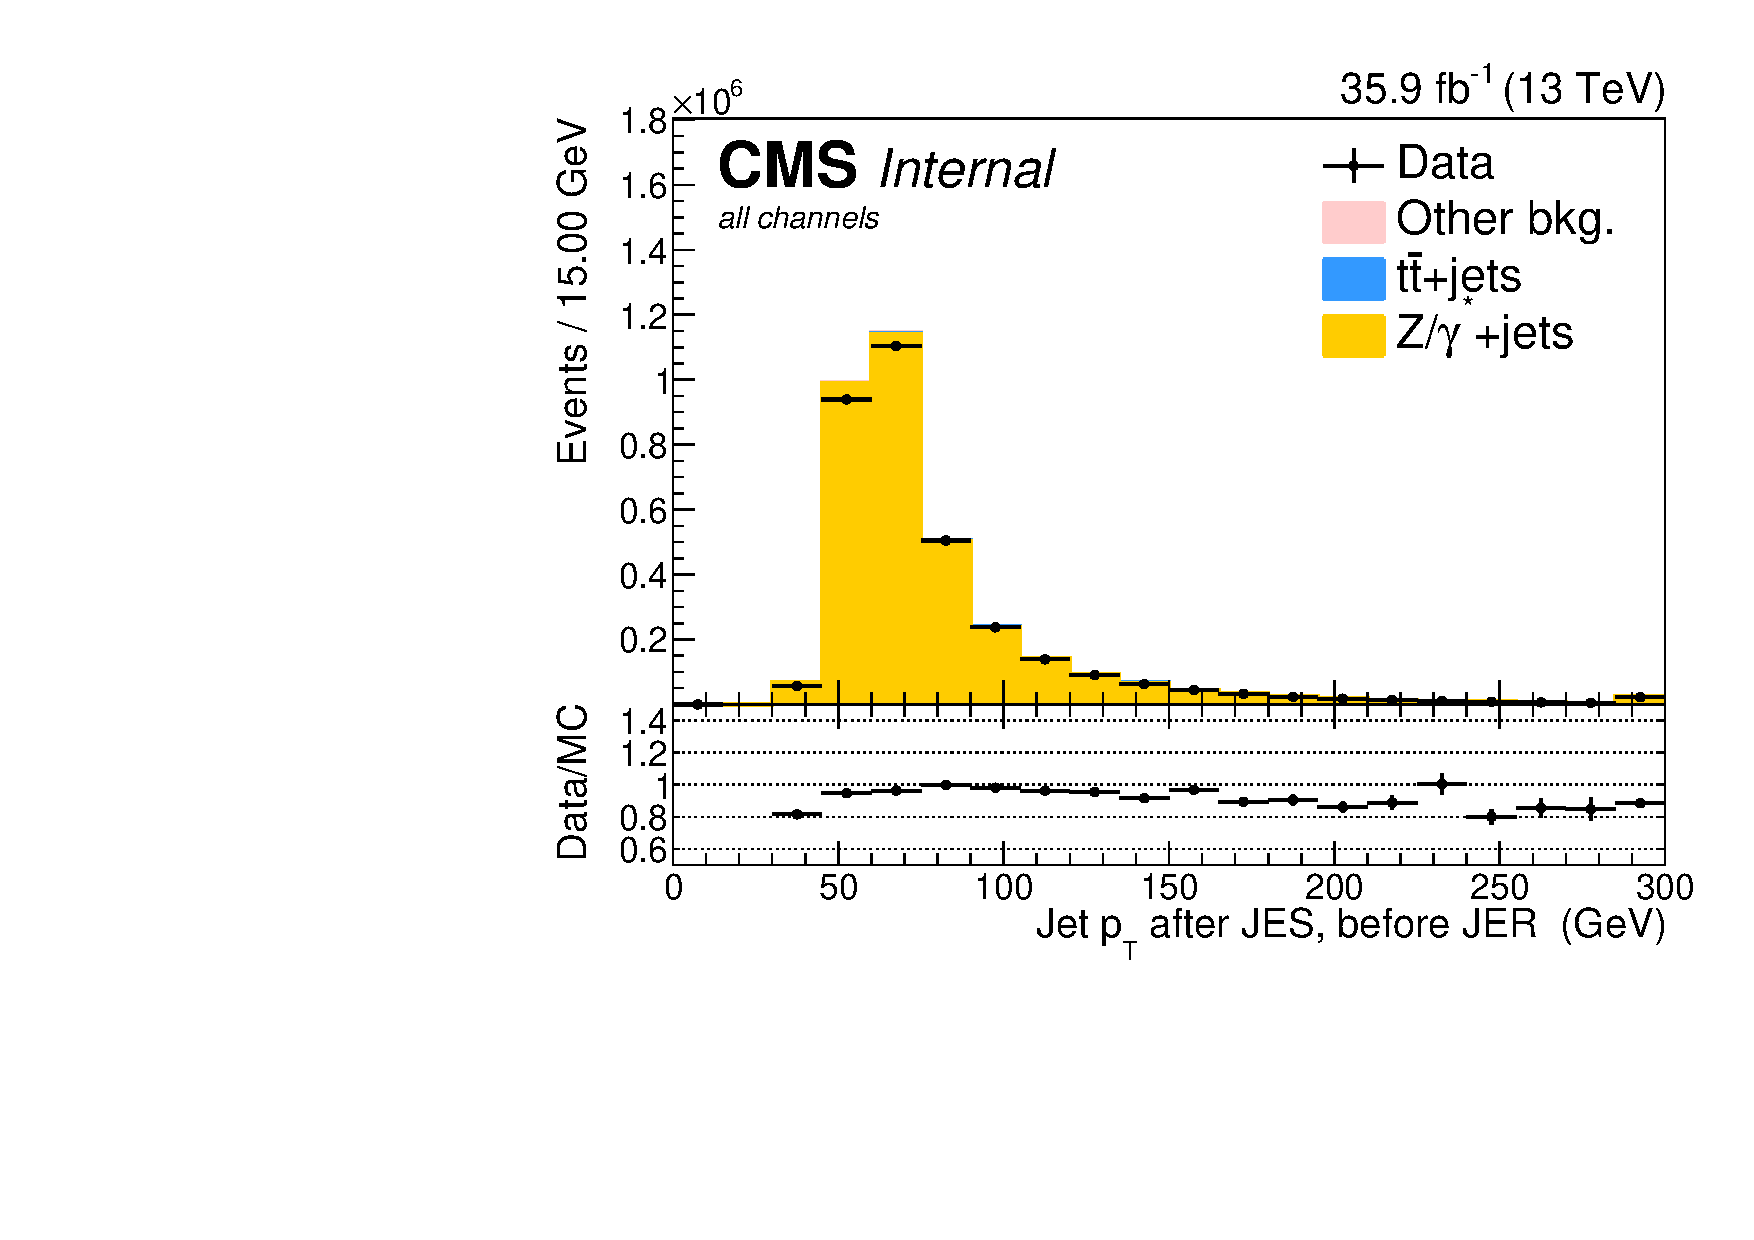
\includegraphics[width=0.49\linewidth]{5_Eventselection/Figures/Reweighing/2lepcontrol_dilep_JetPt_afJES_all_Stack}
	\caption{Distribution of the \pt\ of the jets before (left) and after (right) jet energy scale corrections. Events selected by requiring two leptons in the \PZ\ boson mass window and jets. All other corrections are applied.}
	\label{fig:jesSF}
\end{figure}

\begin{figure}[htbp]
	\centering
	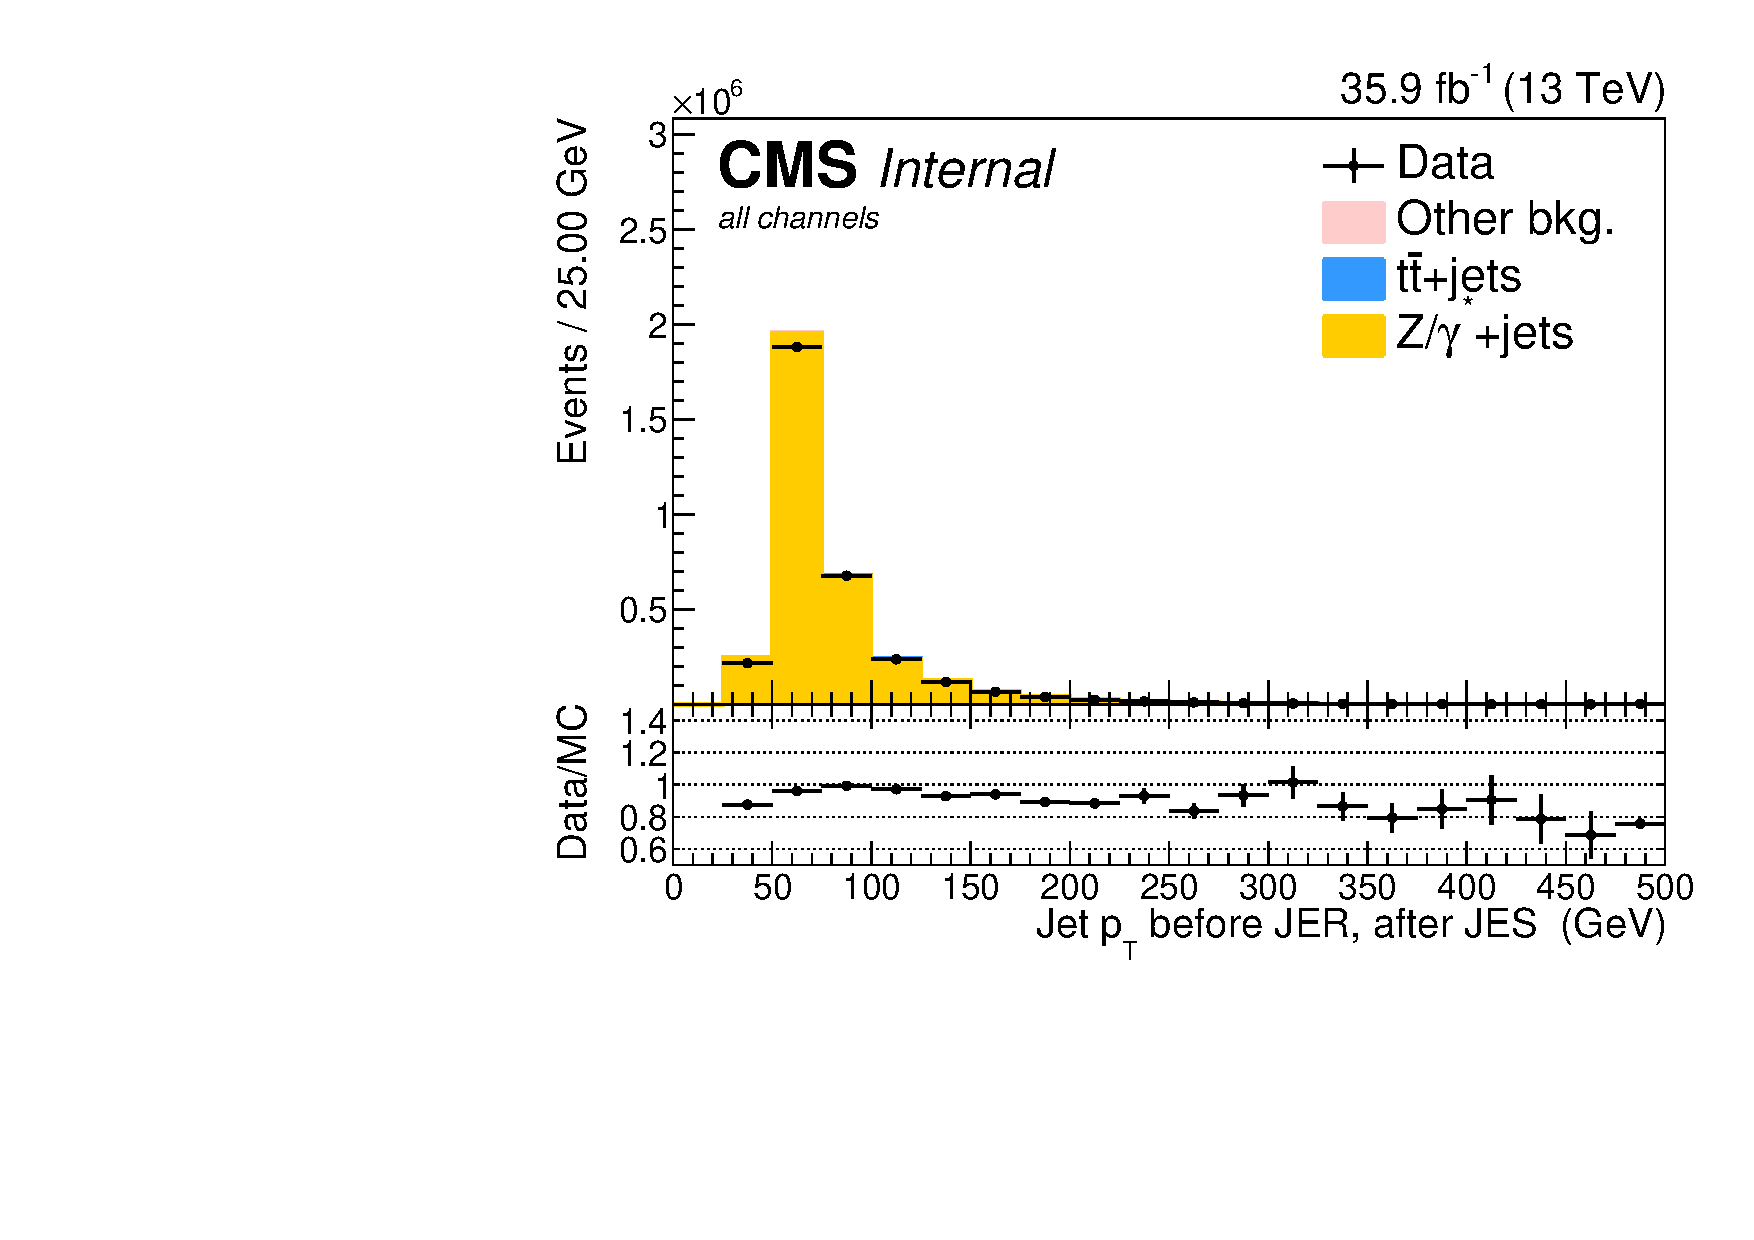
\includegraphics[width=0.49\linewidth]{5_Eventselection/Figures/Reweighing/2lepcontrol_dilep_JetPt_bfJER_all_Stack}
	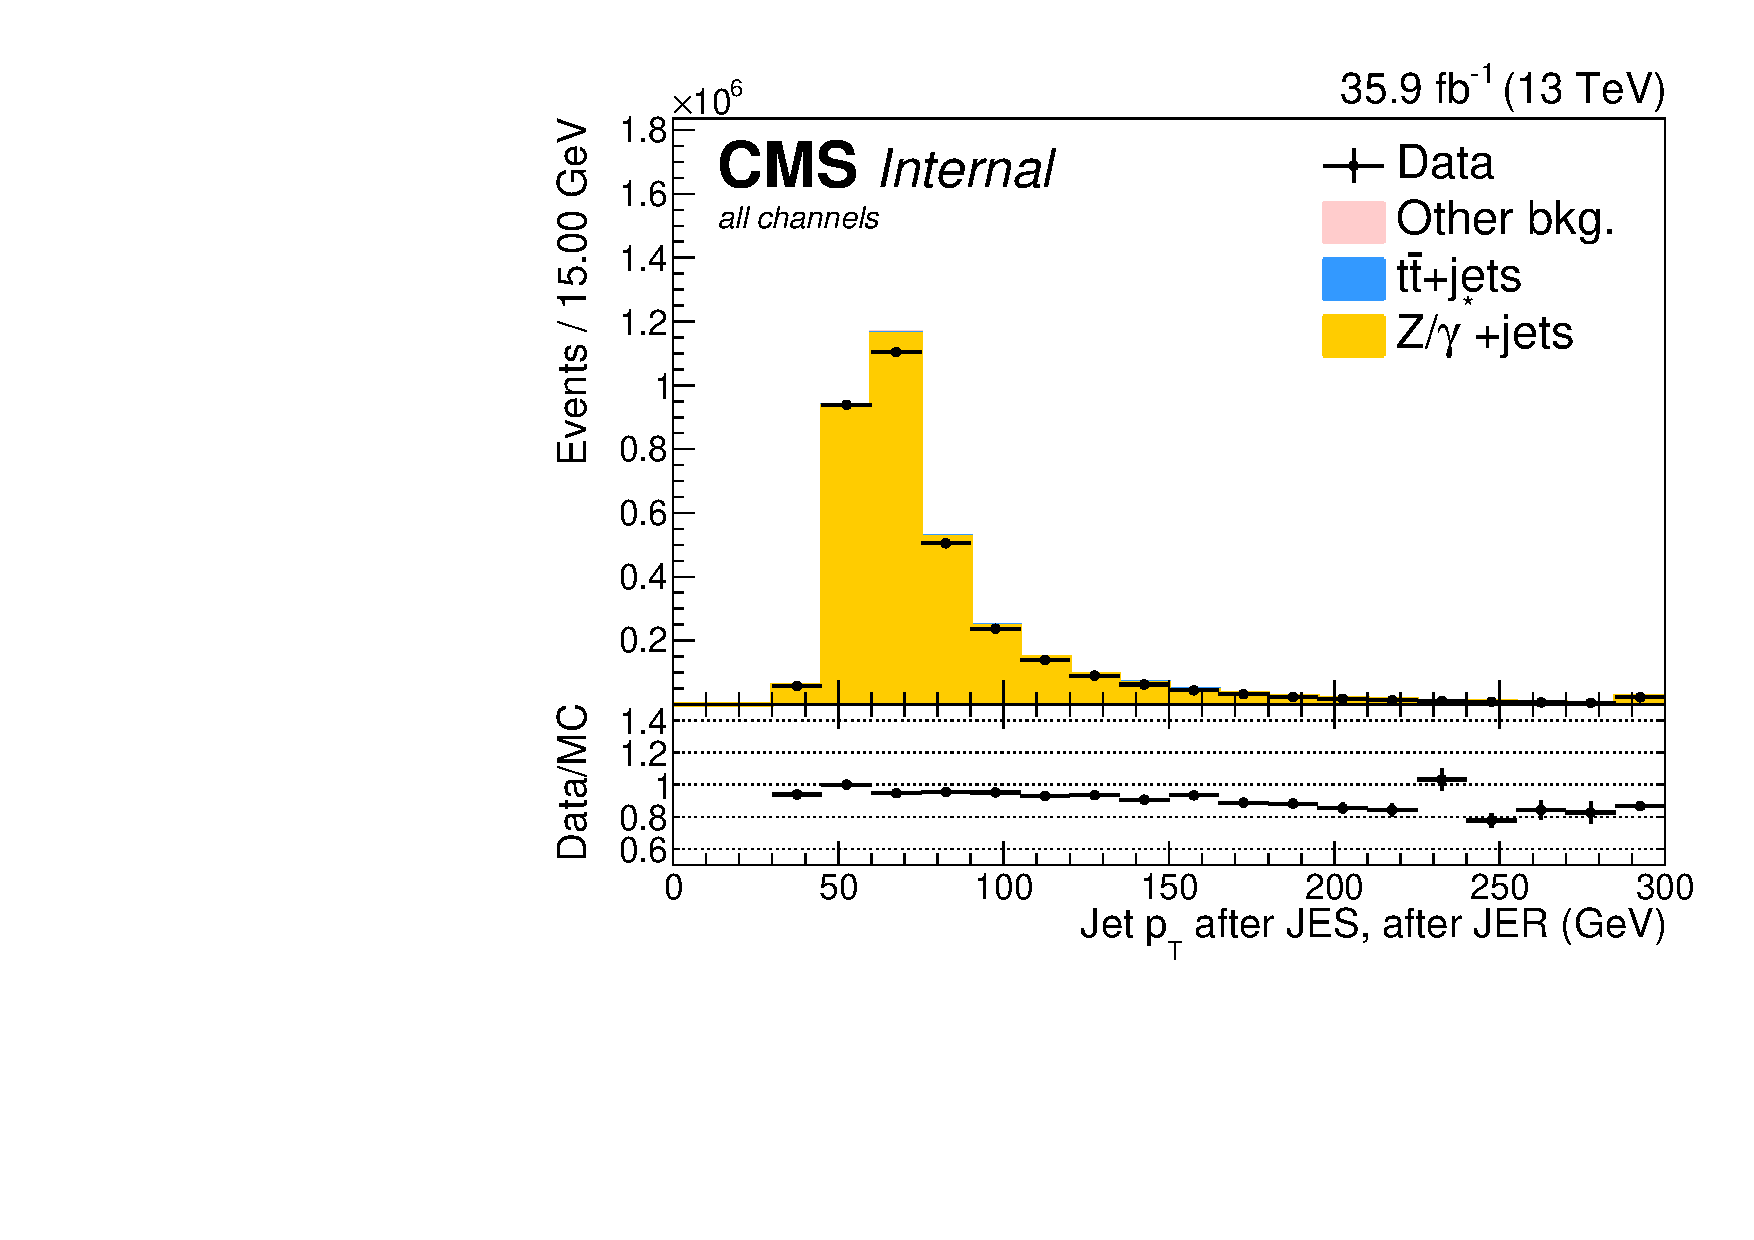
\includegraphics[width=0.49\linewidth]{5_Eventselection/Figures/Reweighing/2lepcontrol_dilep_JetPt_afJER_all_Stack}
	\caption{Distribution of the \pt\ of the jets before (left) and after (right) jet energy resolution smearing. Events selected by requiring two leptons in the \PZ\ boson mass window and jets. All other corrections are applied.}
	\label{fig:jerSF}
\end{figure}



\section{Event reconstruction}
\label{sec:recon}
%After selecting the events, and identifying the objects, the events have to be put reconstructed.  The \PZ\ boson is reconstructed as the sum of the four vectors of the two same flavour leptons of opposite sign giving the closest value to the \PZ\ boson mass. The third remaining lepton is assigned as the lepton coming from the \PW\ boson decay.
%The \SM\ \Pbottom\ jet is assigned to the jet with the highest CSVv2 discriminant. This jet is then removed from the collection of jets. A loop over the jets is performed and the jet that in combination with the reconstructed \PZ\ boson, gives the mass closest to the top mass is assigned as the light flavour jet coming from the FCNC decay of the top quark. The \SM\ top quark candidate is reconstruced by summing the third lepton, the \SM\ b~jet and the neutrino (\Etmis). The longitudinal momentum of the neutrino is calculated by putting a constraint on the lepton + neutrino system with the \PW\ mass. In case two solutions are found for the $p_z^{\nu}$ component, the one that gives the reconstructed mass (lepton + neutrino + b~jet) to  the known top quark mass, is used. 
%
%
%The reconstructed objects are validated using simulation by matching the reconstructed objects to their generated counterpart by minimizing $\Delta R$. The efficiencies derived from the simulated signal samples and the \SM\ \tZq\ background process can be found in \tab{tab:matching} and \tab{tab:matching2}. 
%
%\begin{table}[htbp]
%	\centering
%	\caption{Efficiencies of assigning the correct leptons in the analysis.}
%	\begin{tabular}{cccc}
%		\toprule 
%		& FCNC \tZq  & FCNC \tZ & \SM\ \tZq \\ 
%		\midrule
%		\PW\ lepton & 99\% & 98\% & 97\% \\ 
%	
%		leptons from the \PZ\ boson  & 99\% & 98\% & 97\% \\ 
%		 
%		all leptons in the decay & 99\% & 98\% & 97\% \\ 
%		\bottomrule
%	\end{tabular} 
%	\label{tab:matching}
%\end{table}
%
%
%\begin{table}[htbp]
%	\centering
%	\caption{Efficiencies of assigning the correct jets in the analysis.}
%	\begin{tabular}{cccc}
%		\toprule
%		& FCNC \tZq  & FCNC \tZ & SM \tZq \\ 
%		\midrule
%		\SM\ \Pbottom\ jet & 99\% & 98\% & 80\%\\ 
%		\Pcharm\ jet  & 71\% & N/A & 50\% \\  
%		\Pup\ jet  & 83\% & N/A & 54\% \\ 
%		\bottomrule
%	\end{tabular} 
%	\label{tab:matching2}
%\end{table}
%
%\newpage
After selecting the events,  the objects contained in each event are assigned to physical particles.  The \PZ\ boson is reconstructed as the sum of the four vectors of the two same flavour leptons of opposite electric charge resulting in an invariant mass that is closest to the value of the known \PZ\ boson mass. The third remaining lepton is assigned to the lepton coming from the \PW\ boson decay, so-called \PW\ lepton. This lepton assignment is  validated using simulation by matching the reconstructed objects to their generated counterpart by minimizing  the distance in the distance $\eta\phi$ plane between the true particle and reconstructed one. The efficiencies derived from the simulated signal samples and the \SM\ \tZq\ background process can be found in \tab{tab:matching} for events selected after the three-leptons and jets requirements. The probability that a lepton is assigned to the wrong boson is of the order of a percent for the top quark pair FCNC signal process, and of the order of 2\% for the single top quark FCNC signal process. For the \SM\ \tZq\ process, this probability is 3\%.
\begin{table}[htbp]
	\centering
	\caption{Efficiencies of assigning the correct leptons in the analysis after requiring three leptons and jets.}
	\begin{tabular}{cccc}
		\toprule 
		Origin & FCNC \tZq  & FCNC \tZ & \SM\ \tZq \\ 
		\midrule
		\PW\ boson & 99\% & 98\% & 97\% \\ 
	
		\PZ\ boson  & 99\% & 98\% & 97\% \B\\ 
		 \hdashline
		all leptons in the decay & 99\% & 98\% & 97\% \T \\ 
		\bottomrule
	\end{tabular} 
	\label{tab:matching}
\end{table}

The jet with the highest CSVv2 discriminant is assigned to the b-flavour jet of the SM decay of the top quark, so-called SM b~jet. This jet is then removed from the collection of jets. A loop over the jets is performed and the jet that in combination with the reconstructed \PZ\ boson, gives the mass closest to the known top quark mass is assigned as the light-flavour jet coming from the FCNC decay of the top quark, so-called FCNC jet. The \SM\ top quark candidate is reconstructed by summing the third lepton, the \SM\ b~jet and the neutrino (\Etmis). In \fig{fig:topmass}, the normalized distributions of the invariant mass of the \PW\ lepton and the \SM\ b~jet ($m_{\Plepton_{\PW}b}$), and the invariant mass of the reconstructed \PZ\ boson and FCNC~jet are shown. The distribution of $m_{\Plepton_{\PW}b}$, peaks around 100~\GeV\ for the \FCNC\ signal and \SM\ \ttbar+jets process. The distribution invariant mass of the \PZ\ boson and FCNC jet peaks at the known top mass for the \FCNC\ top quark pair signal. For the single top quark FCNC signal, no extra top is expected and this distribution is smeared out. 
\begin{figure}[tbph]%/171128_1353
	\centering
	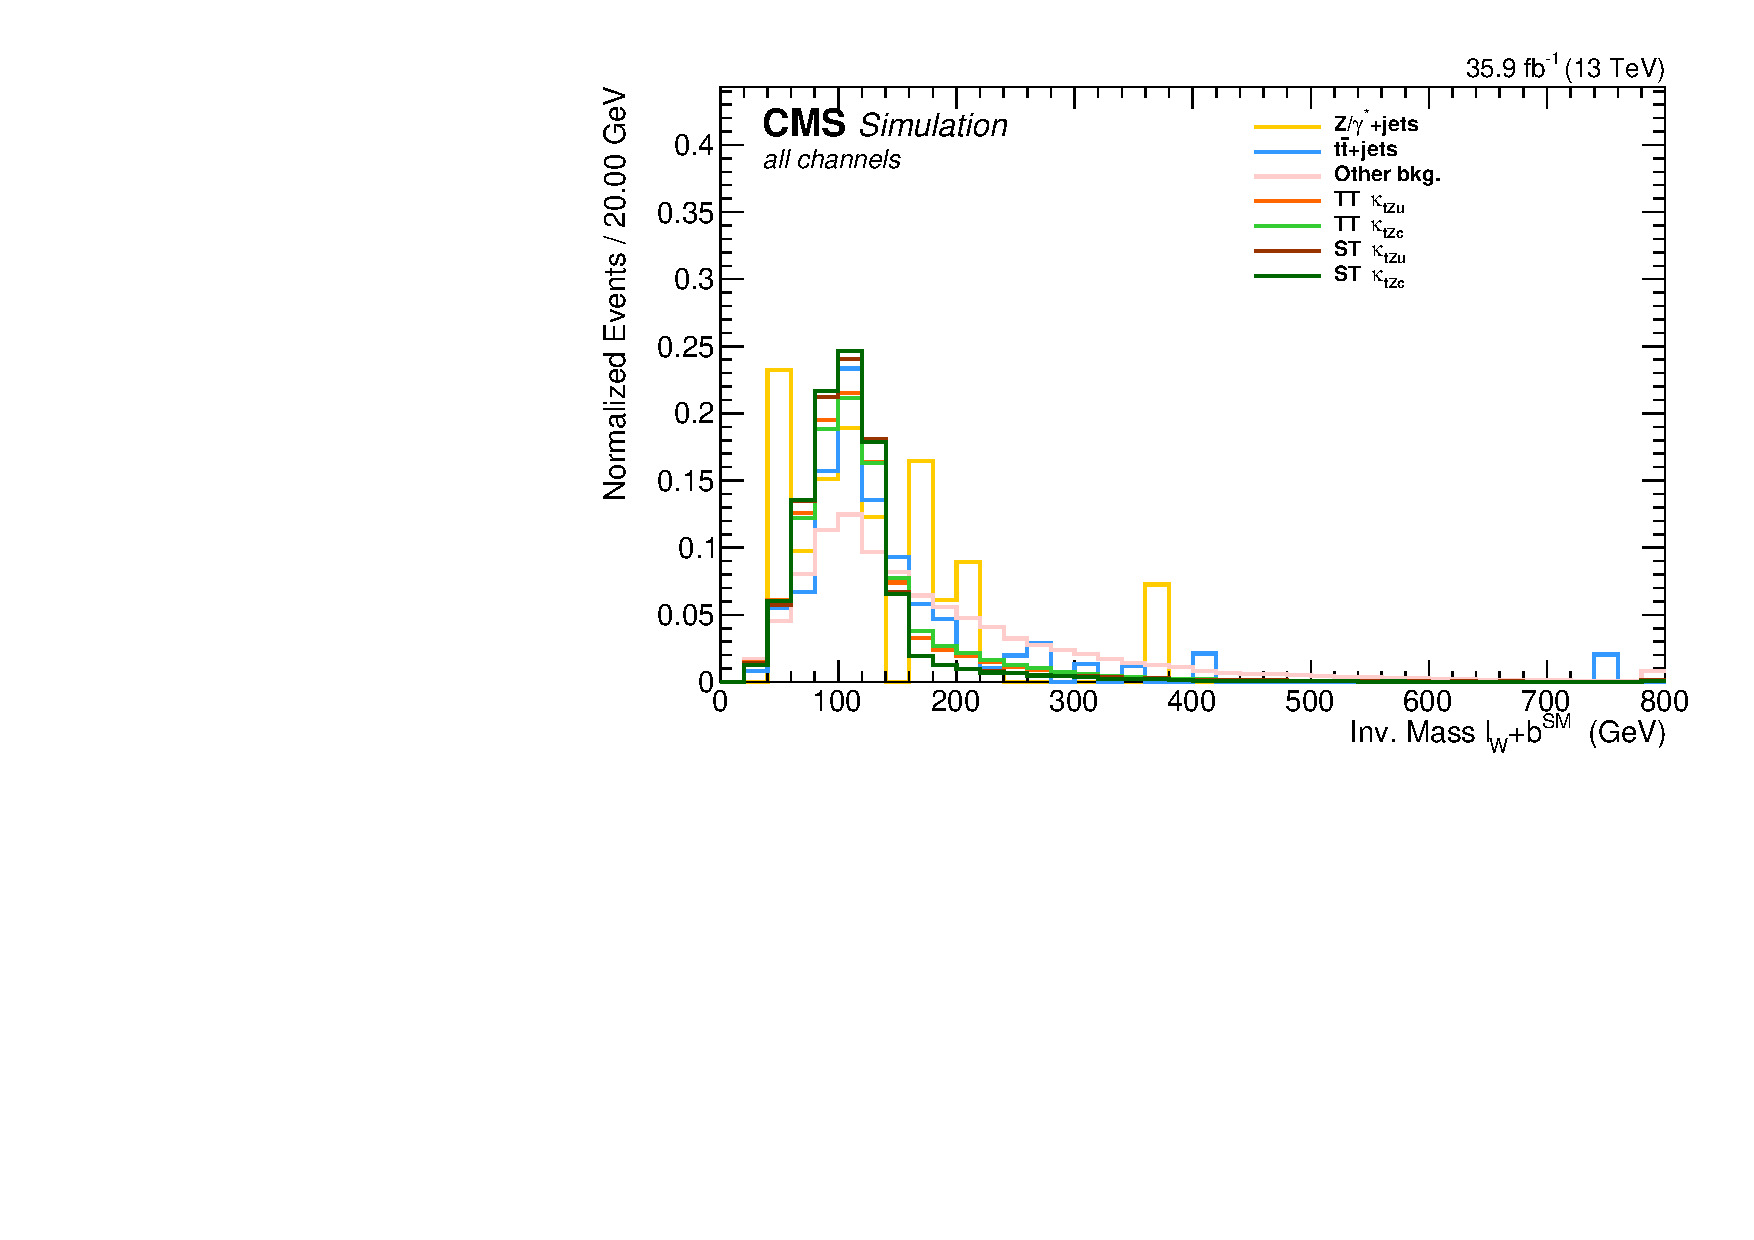
\includegraphics[width=0.49\linewidth]{5_EventSelection/Figures/3lepcontrol_dilep_mlb_all_Normalized}
	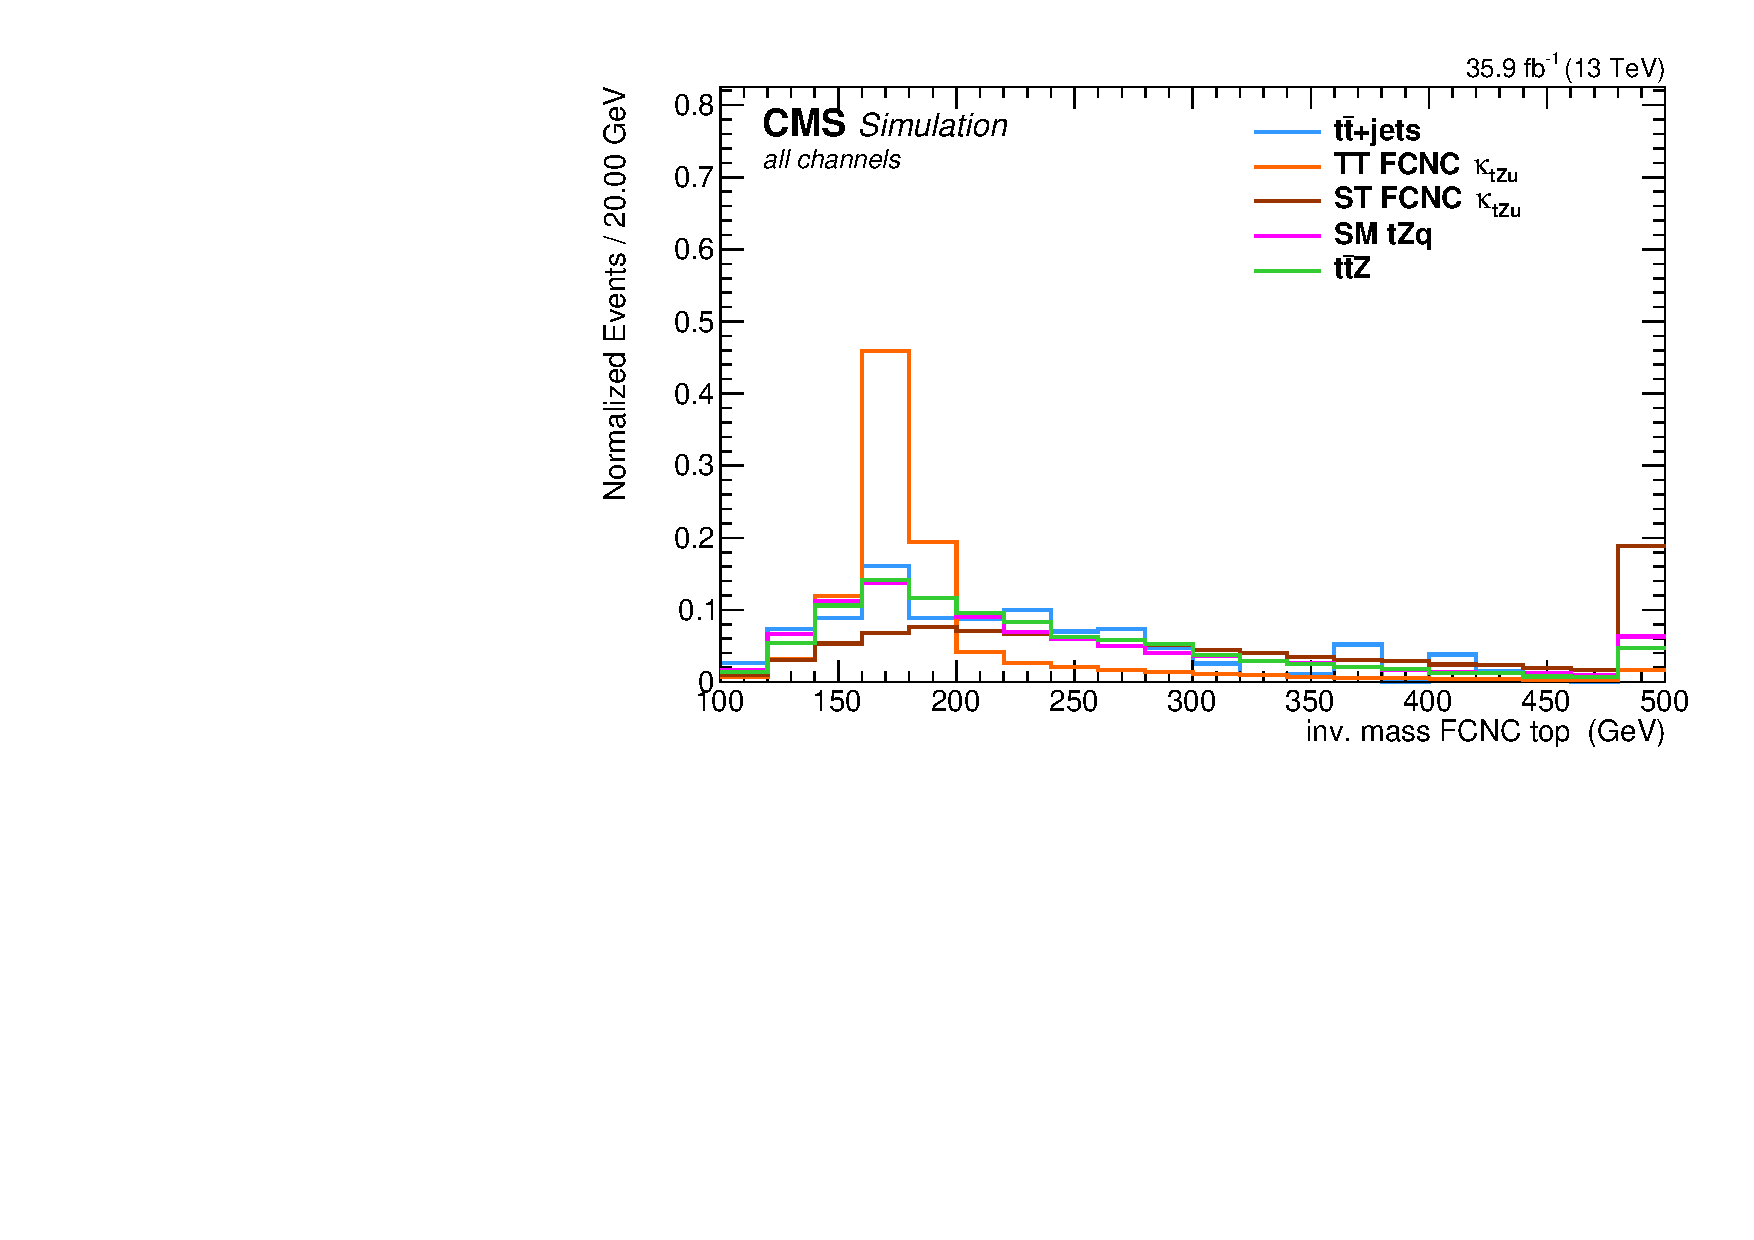
\includegraphics[width=0.49\linewidth]{5_EventSelection/Figures/3lepcontrol_dilep_FCNCTopMass_all_Normalized}
	\caption{Normalised distribution of the invariant mass of the  \PW\ lepton and the \SM\ b~jet (left), and the invariant mass of the reconstructed \PZ\ boson and FCNC~jet (right). After requiring three leptons and jets, in the \PZ\ boson mass window.}
	\label{fig:topmass}
\end{figure}


 The longitudinal momentum of the neutrino is calculated from the missing transverse momentum and the lepton momentum. From momentum conservation follows that 
\begin{equation}
	\vec{p}_{\PW} = \vec{p}_{\Plepton_{\PW}} + \vec{p}_{\Pnu}, 
\end{equation}
and energy conservation requires the \PW\ boson mass squared, 
\begin{equation}
m_{\PW}^2 = \left(80.4~\GeV\right)^2 , 
\end{equation}
is equal to the sum of the transverse momenta of the neutrino \Pnu\ and the lepton $\Plepton_{\PW}$ squared
\begin{equation}
\begin{aligned}
m_{\PW}^2 &\equiv (p_{\Plepton_{\PW}}+ p_{\Pnu})^2.
\end{aligned}
\end{equation}
Assuming that the lepton and neutrino are approximately massless, this equation can be solved for the sought-for $p_{\Pnu}^z$  by setting $p_{\mathrm{T},\Pnu}$ equal to the missing transverse energy in the event. This yields a quadratic equation of the form
\begin{equation}
	 p_{\Pnu,z} = \frac{-b}{2a} \pm \frac{\sqrt{b^2 - 4ac}}{2a} 
\end{equation} 
with 
\begin{equation}
\begin{aligned}
  a &= p_{\Plepton,x}^2 + p_{\Plepton,y}^2, \\
  - b &= m_{\PW}^2 p_{\Plepton,z} + 2 p_{\Plepton,x} p_{\Plepton,z} p_{\Pnu,x} + 2 p_{\Plepton,x} p_{\Plepton,z} p_{\Pnu,y}, \\
  c &=  p_{\Pnu,y} \left( p_{\Plepton,x}^2 + p_{\Plepton,z}^2 \right) + p_{\Pnu,x} \left( p_{\Plepton,x}^2 + p_{\Plepton,z}^2 \right).
\end{aligned} 
\end{equation}
When the solution of this quadratic equation is complex, only the real part ($-b/2a$) is considered. If there are two real solutions, the solution for $p_{\Pnu}^z$ that gives the invariant mass $m_{\Pbottom\Pnu\Plepton_{\PW}}$ closest to the top quark mass (172.9 \GeV) is kept. The normalised distributions of the reconstructed top quark mass and \PW\ boson mass are shown in \fig{fig:topmasss}. For the FCNC signal, the distribution peaks around the known mass of the top quark and has a tail towards higher values. The distribution of the reconstructed \PW\ boson mass peaks at 80~\GeV\ for the FCNC signal.
\begin{figure}[tbph]
	\centering
	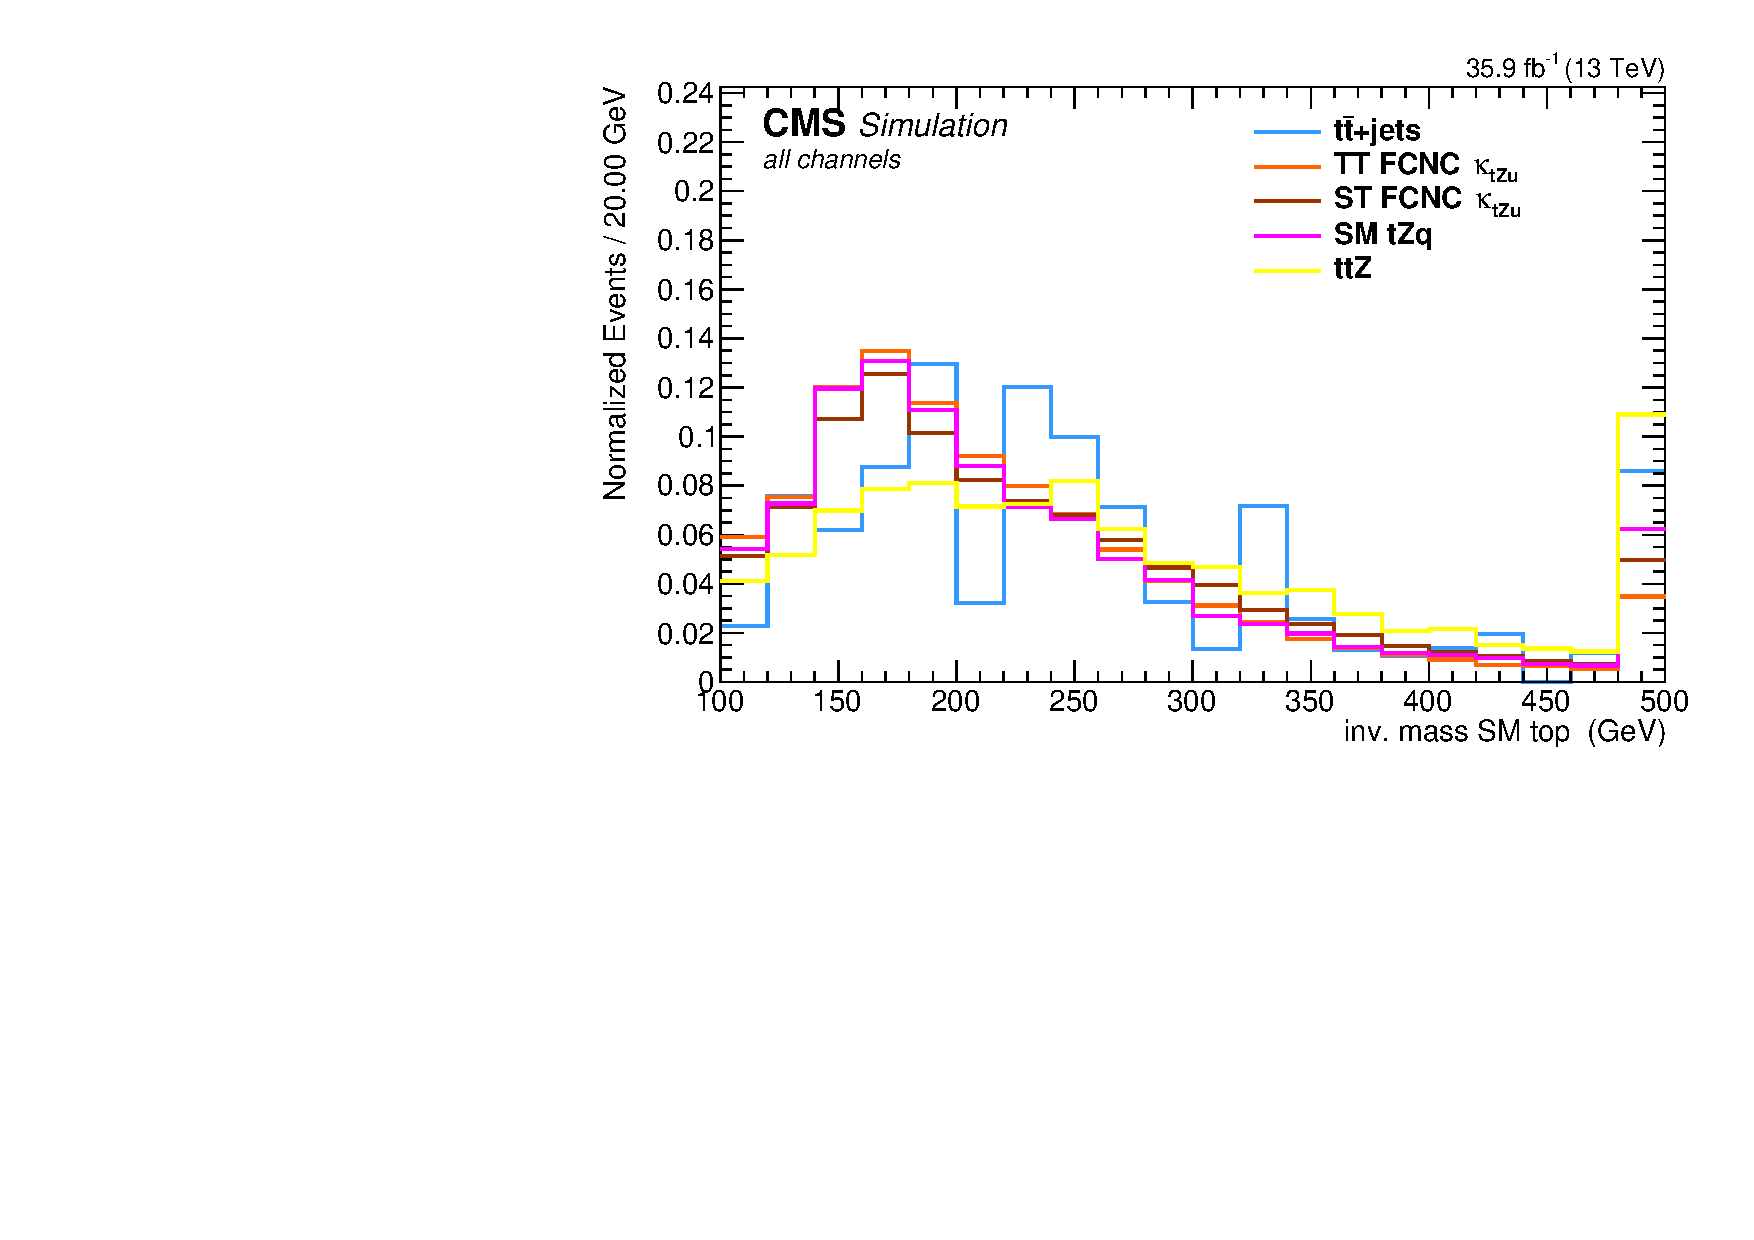
\includegraphics[width=0.49\linewidth]{5_EventSelection/Figures/3lepcontrol_dilep_SMTopMass_all_Normalized}
	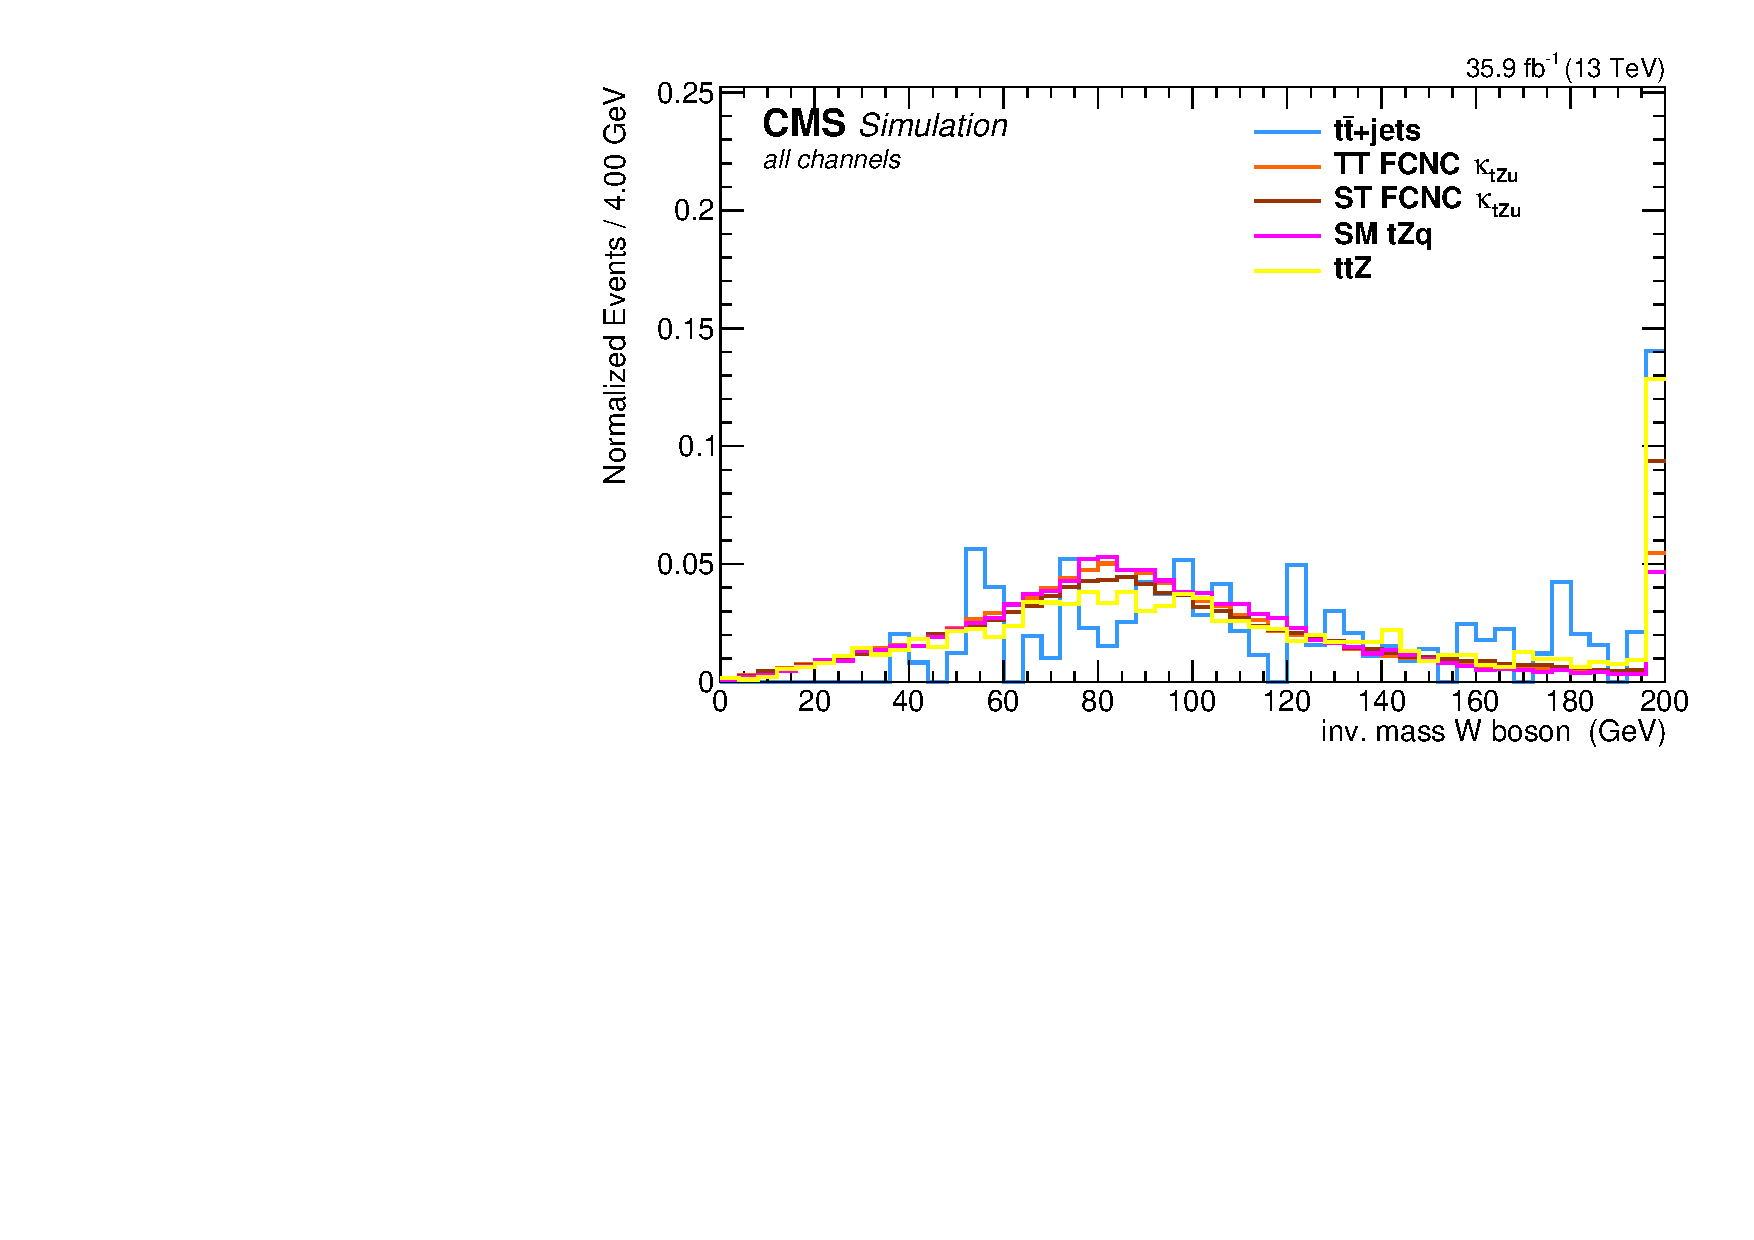
\includegraphics[width=0.49\linewidth]{5_EventSelection/Figures/3lepcontrol_dilep_WbosonMass_all_Normalized}
	\caption{Normalised distribution of the invariant mass of the top quark  decaying via the \SM\ Wtb vertex (left) and the invariant mass of the \PW\ boson. After requiring three leptons and jets, in the \PZ\ boson mass window.}
	\label{fig:topmasss}
\end{figure}
 
\section{Data driven \NPL\ background}
\label{sec:NPL}
% other ways of doing this https://indico.cern.ch/event/283659/contributions/643371/attachments/523063/721480/davidcurtin_fakeleptonsim_MC4BSM_23may2014_v1.key.pdf
 One of the most important backgrounds consists of events with not prompt-leptons (\NPL). Their origin lies mostly in instrumental backgrounds and is therefore very difficult to model. The \NPL\ background  is estimated from data for both its differential distributions and its rate. 

The \NPL\ background  originates from hadronic objects wrongly reconstructed as leptons (so-called fake leptons), or from real leptons coming from the semi-leptonic decay of a \Pbottom\ or \Pcharm\ hadron and from the conversion of photons that pass the identification and isolation requirements (so-called non-prompt leptons). The dominant source of events contained in this \NPL\ background  depends on the flavour of the leptons and therefore the events with a not prompt-muon (\NPM) are treated differently than those with a not prompt-electron (\NPE). For muons, the dominant source is the semi-leptonic decay of heavy flavour hadrons, while for electrons, the dominant sources are hadrons and photon conversions. 

The backgrounds causing events that are contained within the \NPL\ background  are mostly arising from \DY\ (Drell--Yan) and \ttbar+jets dilepton processes, and in a smaller amount from \WW\ processes. All of these processes contain two real leptons and one \NPL. Due to the fact that the probability for a lepton to be a \NPL\ is small, backgrounds containing two or more  not prompt-leptons are neglected in this search. The assumption is made that for the \DY\ process, the two leptons compatible with a \PZ\ boson decay are the real leptons, and the additional lepton is coming from a \NPL\ source. For the \ttbar+jets process, the \NPL\ is assumed to be associated with the \PZ\ boson. This assumption has been validated using Monte Carlo simulations of the \DY\ process and \ttbar+jets process by matching the reconstructed leptons to their true initial generated particles, after requiring exactly three leptons in the Z boson mass window, and jets. For the \DY\ process this assumption is true in 80\% of the events, increasing to 100\% of the events after requiring one b-tagged jet. For the \ttbar+jets process this is true for 60\% of the selected events, and this increases to 90\% after requiring one b-tagged jet.

Since simulation is not able to reproduce the events with not prompt-leptons well, the shape of the distributions for the \NPL\ background sample is constructed from data. Events are selected from data by requiring exactly  two leptons that are identified as real isolated leptons according to the tight working point given in \tab{tab:MuonReq} and \tab{tab:ElecReq}. A third lepton, the so-called not prompt-lepton,  is added by taking a lepton for which the identification criteria are loosened and the isolation citeria are inverted. The full  requirements on the not prompt-leptons are given in \tab{tab:nonpromptel} and \tab{tab:nonpromptmu}. For not prompt-electrons, a large fraction is coming from misidentified photons. These are removed by applying a tighter cut on the $1/E-1/p$ variable, and by limiting the isolation values to be smaller than one, in coherence with the \SM\ \tZq\ search from CMS~\cite{CMS-PAS-TOP-16-020}. 

The normalisation of the distributions from the \NPL\ background sample is estimated from data through the use of control regions that are fitted simultaneously with the signal regions. These regions are defined in \Sec{sec:regions}.
\begin{table}[htbp]
	\centering
	
	\caption{Not prompt-electron requirements used in this analysis. The requirements for electrons are set in the barrel ($|\eta_{supercluster}| \leq 1.479$)
		and the end caps ($|\eta_{supercluster}| > 1.479$). }
	\begin{tabular}{ccc}
		\toprule
	 Properties	& \multicolumn{1}{c}{$|\eta_{supercluster}| \leq 1.479$ } & \multicolumn{1}{c}{$|\eta_{supercluster}| > 1.479$ } \\
		\midrule
		$\sigma_{\eta \eta}$ & $<$ 0.011 & $<$ 0.0314 \\ 
		
		$|\Delta\eta_{\mathrm{in}}|$ & $<$ 0.00477& $<$ 0.00868\\ 
		
		$|\Delta\phi_{\mathrm{in}}|$ & $<$ 0.222 &  $<$ 0.212 \\ 
		 
		H/E & $<$ 0.298& $<$ 0.101 \\ 
		
		relative isolation & $\left[ 0.0588  , 1\right[$ &  $\left[ 0.0571, 1\right[$\\ 
	
		$|1/E-1/p|$ (\GeVinv) & $<$ 0.0129  & $<$ 0.0129  \\ 
		
		expected missing inner hits & $\leq $ 1 &  $\leq $ 1\\ 
	
		 conversion veto & Y & Y \\ 
	
		\pt\ (\GeV) &$>$ 35 & $>$ 35  \\
		\bottomrule
	\end{tabular} 
	\label{tab:nonpromptel}
\end{table}

\begin{table}[htbp]
	\centering
	\caption{Not prompt-muon requirements used in the analysis. }
	
	\begin{tabular}{cc}
		\toprule
	 Properties	& modified Loose Muon WP \\ 
		\midrule 
		Global muon or Tracker Muon & Both  \\ 
		
		Particle Flow muon & Y  \\ 
		
		$\chi^2/\mathrm{ndof}$ of global muon track fit & N/A \\  
		
		Nb. of hit muon chambers & N/A \\ 
		 
		Nb. of muon stations contained in the segment & N/A   \\ 
		
		Size of the transverse impact parameter  of the track wrt. PV & N/A  \\ 
		 
		Longitudinal distance wrt. PV & N/A \\ 
		
		Nb. of pixel hits & N/A \\ 
		
		Nb. of tracker layers with hits & N/A  \\ 
		
		Relative Isolation & $\leq 0.15$ \\
		
		\pt\ (\GeV) &$>$ 30  \\
		\bottomrule
	\end{tabular} 
	
	\label{tab:nonpromptmu}
\end{table}


\newpage
\section{Analysis Strategy}
\label{sec:regions}

The baseline selection of this analysis selects events where jets and three leptons are present. Additional leptons with a looser identification are vetoed in order to reduce the contamination of backgrounds with four or more leptons in the final state, e.g. \ZZ, \ttZ, and \ttH. This makes that the most important backgrounds in this search consist of backgrounds  that contain three prompt leptons in the final state. These are mainly \WZ +jets, \ttZ\ and SM \tZq. For these backgrounds, the three lepton topology is identical to the \FCNC\ signal: two opposite sign leptons of the same flavour decaying from the \PZ\ boson, and a third additional, high \pt\ lepton coming from the \PW\ boson decay.

For the single top quark FCNC final state, one \Pbottom\ jet coming from the \SM\ top quark decay is expected. For the top quark pair FCNC signal, an additional light-flavour jet is expected. In the \ttZ\ final state, two b~jets are present in the final state. However, due to inefficiencies of the b-tagging algorithm, one of the two \Pbottom\ jets may be identified as a light-flavour jet, giving the same final state as the top quark pair FCNC final state. For the \WZ+jets final states, one of the b~jets produced by gluon splitting, can be b-tagged or light-flavour jets coming from the \WZ+jets production can be mis-tagged as b~jets. The SM \tZq\ final state expects the same signal as the top quark pair FCNC process. Furthermore, the \NPL\  background is responsible for a  significant amount of background events. 

In \fig{fig:controldilepdecaystacklogy}, the number of events per leptonic decay are shown. In the dilepton channels, the data and simulation agrees. For the three lepton decays, there is poor agreement due to the fact that the \NPL\ background is not well simulated.  For this reason, the \NPL\ background will be estimated in a data-driven way and the simulated samples of \DY, \ttbar+jets and \WW\ will not be used as explained in \Sec{sec:NPL}. One can also see that in the three lepton channels, the other backgrounds become more important, these are mainly \WZ+jets, \SM\ \tZq, \ttZ\ and \ZZ\ processes.
\begin{figure}[htbp]
	\centering
	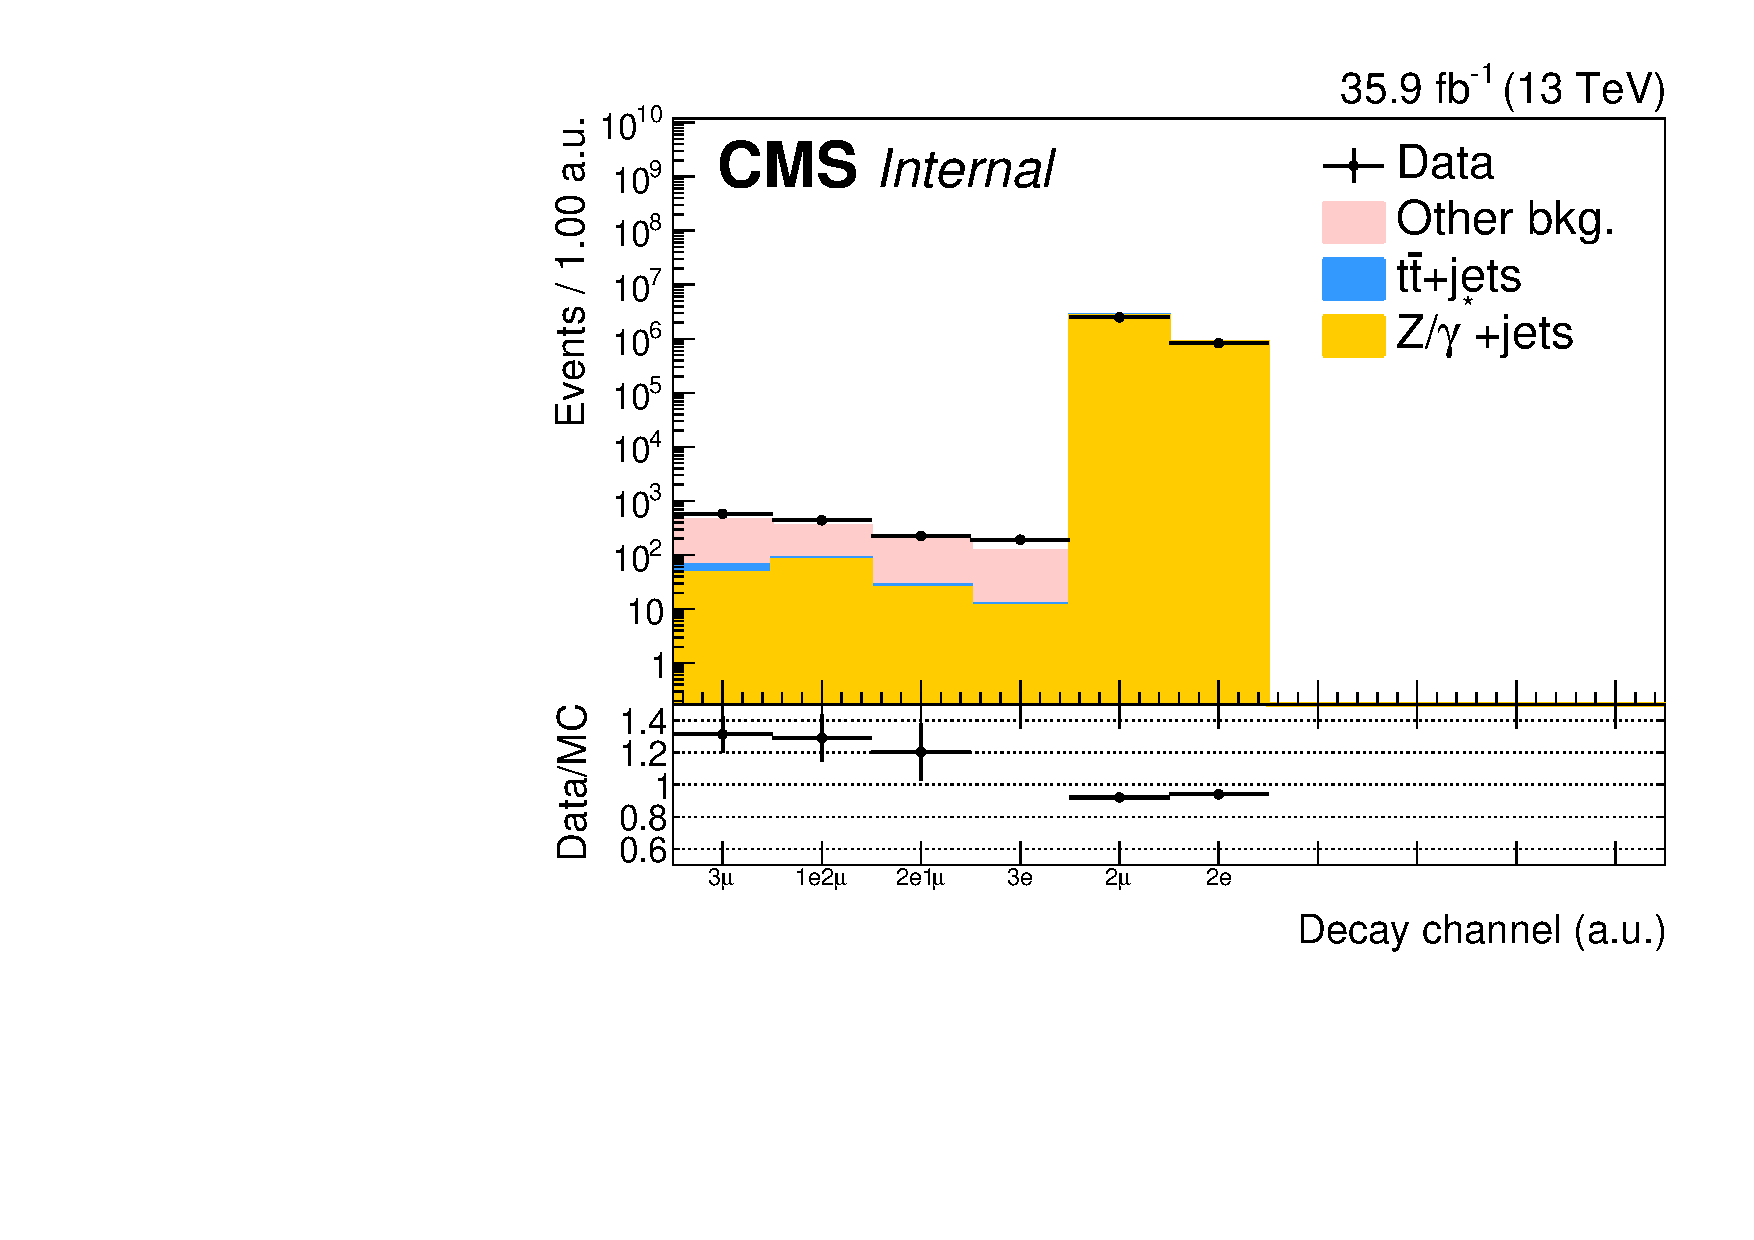
\includegraphics[width=0.58\linewidth]{5_EventSelection/Figures/control_dilep_Decay_StackLogY.pdf}
	\caption{Number of events per leptonic-decay after requiring at least two or exactly three leptons and jets, in the \PZ\ boson mass window. The different decays are not exclusive. }
	\label{fig:controldilepdecaystacklogy}
\end{figure}



The analysis strategy is shown in \fig{fig:regions}. Based on the jet multiplicity, the b-tag information and the reconstructed \PZ\ boson mass, five statistically independent regions are defined after a common selection of exactly three leptons containing one opposite sign same flavour pair that is assigned to the \PZ\ boson, at least one jet and at the most three jets, and the transverse mass of the \PW\ boson to be maximal 300~\GeV. The requirements for each region are shown in \tab{tab:Regions}. Two signal regions are considered, targeting the final state of each of the single top quark and top quark pair signals. The \STSR\ is constructed to target the final state of the single top quark FCNC signal, while the \TTSR\ is constructed to target the top quark pair FCNC signal. In each signal region, a multivariate discriminant based on Boosted Decision Trees (BDT) (see \Sec{sec:BDT}) is used to respectively discriminate single top quark \FCNC\ and top quark pair \FCNC\ signal from backgrounds. The rate of \WZ+jet events as well as that of the \NPL\ background, mainly originating from the \DY\ process, is estimated in the \WZCR. Here, the transverse mass of the \PW~boson \mtw\ that is defined as function of the lepton $l_{\PW}$ assigned to the \PW~boson and the neutrino  $\nu_{\W}$ coming from the missing transverse energy in the event
\begin{equation}
\mtw = \sqrt{\left(\pt(l_{\W}) + \pt(\nu_{\W}) \right) ^2 - \left(p_{\mathrm{x}}(l_{\W}) + p_{\mathrm{x}}(\nu_{\W})\right)^2  - \left(p_{\mathrm{y}}(l_{\W}) + p_{\mathrm{y}}(\nu_{\W})\right)^2    } ,
\end{equation}
 is used as  discriminating variable between the two background processes, \WZ+jets and \NPL. The normalisation of the backgrounds is then used in the signal regions via the b-tagging information (\Sec{sec:WZCR}). The \NPL\ background coming from a \ttbar+jets process is constrained by two control regions, \TTCR\ and \STCR, one for each signal region (respectively \TTSR\ and \STSR).  The normalisation of the \ttbar+jets process is estimated by subtracting all other background predictions from the data rate (\Sec{sec:TTCR}). A simultaneous global fit using the \texttt{Higgs Combined Tool} (\Sec{sec:Stat}) is performed taking into account each region (\STSR, \TTSR, \WZCR, \TTCR\ and \STCR) for the four different three-lepton channels. The BDTs in the signal regions, as well as the transverse mass of the \PW\ boson are discussed in \Chap{chap:6}. The number of events for each region are shown in \Sec{sec:Yields}.
\begin{figure}[htbp]
	\centering
	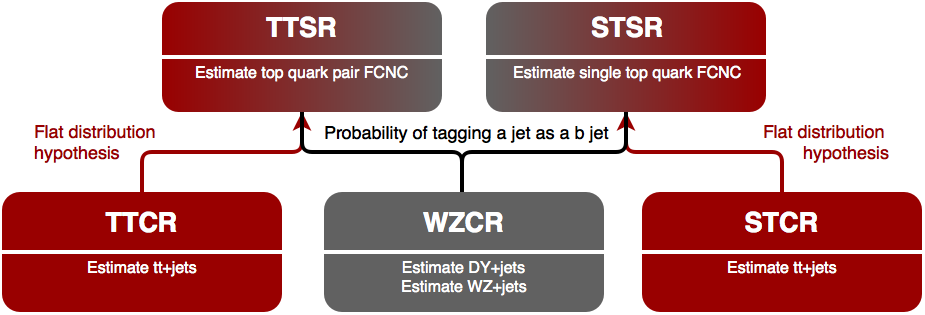
\includegraphics[width=1.\linewidth]{5_EventSelection/Figures/regions}
	\caption{The strategy used for the search presented in this thesis. The \WZCR\ region is used to estimate the \WZ+jets background process as well as the \NPL\ background coming from the \DY\ process. The \TTCR\ and \STCR\ regions are used to estimate the contributions of the \NPL\ background coming from the \ttbar+jets process.}
	\label{fig:regions}
\end{figure}

%The regions are defined as in \tab{tab:Regions} after a common selection of exactly three leptons containing one opposite sign same flavour pair that is assigned to the \PZ\ boson, at least one jet and at the most three jets, and the transverse mass of the \PW\ boson to be maximal 300 \GeV. %The cut on the transverse mass of the \PW\ boson is done to remove events that are passing the events cleaning elading to anomalous large missing transverse energy.
%The transverse mass $\mtw$ is reconstructed using
%\begin{equation}
%\mtw = \sqrt{\left(\pt(l_{\W}) + \pt(\nu_{\W}) ) ^2 - (p_{\mathrm{x}}(l_{\W}) + p_{\mathrm{x}}(\nu_{\W}))^2  - (p_{\mathrm{y}}(l_{\W}) + p_{\mathrm{y}}(\nu_{\W})\right)^2    } .
%\end{equation}

\begin{table}[htbp]
	\centering
	\caption{The statistically independent regions used in the analysis.}
	\begin{tabular}{cccccc}
		\toprule
%		& \WZ  & \tZ  & \tZq  & \tZ  & \tZq\\ 
%		&  control region &  signal region & signal region &  control region & control region\\ 
		& \WZCR& \STSR  & \TTSR & \STCR & \TTCR \\ 
		\midrule
		Number of jets & $\geqslant 1$ & 1 & $\geqslant 2$  & 1 & $\geqslant 2$\\ 
		 
		Number of b~jets & 0 & 1 & $\geqslant 1$  & 1 & $\geqslant 1$ \\ 
		
		$|\mZ^{\mathrm{reco}} - \mZ|< 7.5$ \GeV & Yes & Yes & Yes & No & No \B\\
		\hdashline
		$|\mZ^{\mathrm{reco}} - \mZ|< 30$ \GeV & Yes & Yes & Yes & Yes & Yes \T\\
			Number of leptons & 3 & 3 & 3  & 3 & 3\\
		\bottomrule 
	\end{tabular} 
	\label{tab:Regions}
\end{table}


%In order to reduce the large uncertainties in backgrounds, five independent regions are used as defined in  \tab{tab:Regions}. In \fig{fig:regions}, the strategy and usage of each region is illustrated.


\subsection{WZCR}
\label{sec:WZCR}
The \WZCR\ is constructed by vetoing events with jets tagged as being a b~jet, making it statistically independent from the signal regions where at least one b-tagged jet is required. In this control region, a fit is performed on the transverse mass of the \PW\ boson, in order to estimate the \NPL\ yield coming from \DY\ and the \WZ+jets backgrounds. 

A transfer factor is used to project the yield in the region without b-tagged jets to the regions with exactly, or at least, one  b-tagged jet. For this, the probability of tagging at least one jet with the CSVv2 algorithm at the loose working point is used to calculate the expected number of events, $N_b$, after b-tagging: 
\begin{equation}
	N_{\mathrm{b}} = \frac{\sum \limits_{\mathrm{events}}\mathcal{P}_b}{\text{total nb of events}},
\end{equation}
where $\mathcal{P}_{\mathrm{b}}$ is the probability that an event survives the b-tagging requirement,
\begin{equation}
\begin{aligned}
	\mathcal{P}_{\mathrm{b}} =& 1 - \text{P(event does not survive b tag)},\\
	 =& 1 - \left(\prod_{\Pbottom} \text{P(b not b-tagged)} \prod_{\Pcharm} \text{P(c not b-tagged)} \prod_{\mathrm{udsg}} \text{P(light not b-tagged)}\right),
%	& = 1 - \left(\prod_{b} 0.10 \prod_{c} 0.40 \prod_{udsg} 0.90\right)
\end{aligned}
\end{equation}
with the products going over all b-, c-, and light-flavour jets respectively. The jet flavour is determined by means of matching the reconstructed jet to the generated quarks, based on the distance in the $\eta\phi$ plane. In order to estimate the probability for exactly one b-tagged jet, the expected number of events is corrected by the fraction of events with exactly  one jet in the \WZCR. The resulting transfer factors are given in \App{app:tablestr}. The yield of \WZ+jets events in the signal region estimated using the above described transfer factor, and the yield calculated with simulated events, are in agreement. 
\subsection{\TTSR\ and \STSR}
The \TTSR\ is defined to target the top quark pair FCNC (\tZq) process, while the \STSR\ focusses on the single top quark FCNC (\tZ) process. They have \NPL\ contributions coming from \DY\ and \ttbar+jets events. In these regions, the data driven \NPL\ template is split into two templates, based on the presence of the \NPL\ in the Z boson. The \NPL\ associated with \PW\ boson is assigned to \DY\ and its yield is estimated in the \WZCR, while  the \NPL\ associated with \PZ\ boson is assigned to \ttbar+jets and its yield is estimated in the \TTCR\ and \STCR.

\subsection{\TTCR\ and \STCR}
\label{sec:TTCR}
The \TTCR\ and \STCR\  are constructed with the same selection criteria as \TTSR\ and \STSR, but are outside the \PZ\ boson mass window, i.e side-bands defined as
\begin{equation}
7.5 \:\GeV < |\mZ^{\mathrm{reco}} - \mZ| < 30 \:\GeV,
\end{equation}
where $\mZ^{\mathrm{reco}}$ is the reconstructed mass of the \PZ\ boson in the event, and $\mZ$ the  known mass of the \PZ\ boson.
These regions are dominated by \ttbar+jets (see \App{app:tablestr}) and are used to estimate the \NPL\ background event yield coming from the \ttbar+jets process in the \STSR\ and \TTSR. Since there are few events entering the \STCR\ and \TTCR, no shapes are used in the fit, i.e. only the absolute event yield is used. The distribution of the mass of the Z boson is flat for \ttbar+jets events, as shown in \fig{fig:3lepcontrolafteratleast1jet3lepzbosonmassallnormalized},  and thus the number of expected events, $N_s$, in the signal regions estimated from the number of expected events, $N_c$, in the control region is obtained as
\begin{equation}
N_s = \frac{15}{60-15} N_c.
\end{equation}
The resulting transfer factors are given in \App{app:tablestr}. The expected yield in the signal region estimated from the \TTCR\ (\STCR) is in agreement with the yield calculated from simulated events. 
\begin{figure}[htbp]
	\centering
	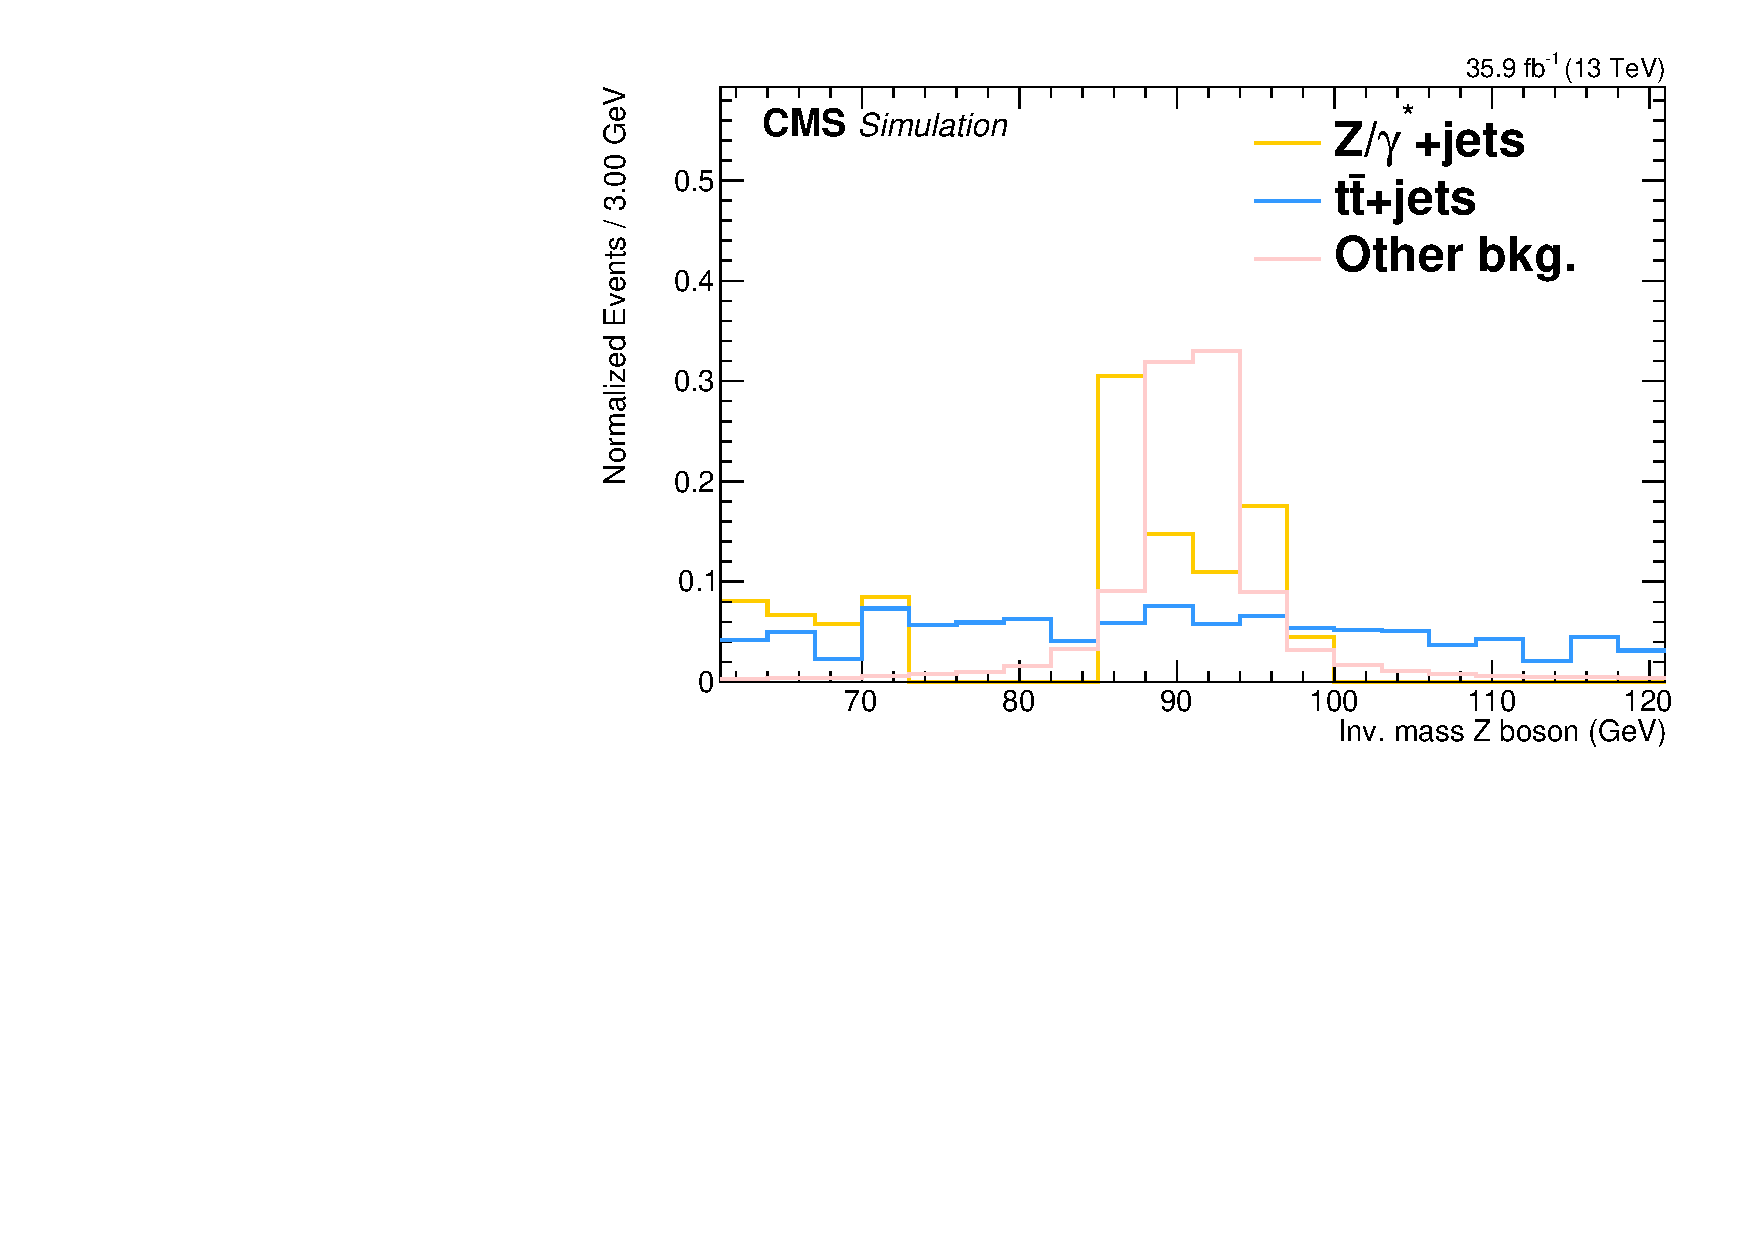
\includegraphics[width=0.7\linewidth]{5_EventSelection/Figures/zbosonmass_Normalized}
	\caption{The normalized distribution for \DY\ and \ttbar+jets events before dividing the events into regions, after $|\mZ^{\mathrm{reco}} - \mZ| < 30$~\GeV. All three-lepton channels combined. }
	\label{fig:3lepcontrolafteratleast1jet3lepzbosonmassallnormalized}
\end{figure}

%It is shown in \App{app:BDTnp}, that these two templates have the same shape within the limited statistics, not assuming any systematic uncertainties. 
\newpage
\subsection{Event yields}
\label{sec:Yields}
\begin{comment}
	//Return integral of bin contents in range [binx1,binx2] and its error 
   // By default the integral is computed as the sum of bin contents in the range.
   // if option "width" is specified, the integral is the sum of
   // the bin contents multiplied by the bin width in x.
   // the error is computed using error propagation from the bin errors assumming that 
   // all the bins are uncorrelated
   if Sumw2 has been called, the error per bin is computed as the sqrt(sum of squares of weights), otherwise the error is set equal to the sqrt(bin content).
   
\end{comment}
In this section, the event yields for each region are given. In \tab{tab:YieldSTCR} and \tab{tab:YieldTTCR} the event yields in the side-band control regions, \STCR\ and \TTCR, are given.  \tab{tab:YieldWZCR} contains the event yields for the \WZCR. The event yields in the signal regions, \STSR\ and \TTSR, are given in \tab{tab:YieldSTSR} and \tab{tab:YieldTTSR} respectively. The background yields follow the relative fractions predicted by the simulation. The \NPL\ background is constructed from a dilepton sample with an extra not prompt-lepton. For this reason, the NPL sample is normalised to reach a total background yield equal to the observed data yield. The actual yield will be taken from data during the global fit as explained in the previous section.  The signal yield is set to its expected value for branching fraction equal to the expected limits of most stringent upper limit set by CMS~\cite{Sirunyan:2017kkr} at 95\% CL, being $\BR(\Ptop \rightarrow \Pup\PZ) <  2.7  \times 10^{-4}$ and  $\BR(\Ptop \rightarrow \Pcharm\PZ) < 12 \times 10^{-4}$. 

From the tables one can see that for the \TTCR\ and the \STCR, the main contribution should come from the \NPL\ background, making this control region well defined for estimating the yield of this background. The \WZCR\ is dominated by the \WZ+jets process and also here a large contribution of the \NPL\ background is expected. In the \STSR, the main background is the \NPL\ background, followed by the \SM\ \tZq, and \WZ+jets process. For the \TTSR, the main background is also the \NPL\ background, followed by the \ttZ\ process, \SM\ \tZq\ process and \WZ+jets process. 

  \begin{table}[htbp]
	\centering
	\caption{Event yields in the \STCR. The signal yield is set to its expected value for branching fraction equal to the expected limits of most stringent upper limit set by CMS~\cite{Sirunyan:2017kkr}, being $\BR(\Ptop \rightarrow \Pup\PZ) <  2.7  \times 10^{-4}$ and  $\BR(\Ptop \rightarrow \Pcharm\PZ) < 12 \times 10^{-4}$. The yield of the \NPL\ background will be taken from the fit.   }
	\begin{tabular} {l c c c c c  }
		\toprule
		Process & all channels & \mumumu\ channel & \emumu\ channel & \eemu\ channel &\eee\ channel  \\
		\midrule
		\NPL\ \ttbar   & 24.02 & 8.70  & 14.04  & 0.83  & 0.45  \\ 
		\ttZ 				&  0.18 $ \pm $ 0.21 &  0.09 $\pm$ 0.06 &  0.03 $\pm$ 0.21 & 0.02 $\pm$ 0.03 & 0.04 $\pm$ 0.03 \\ 
		\WZ 				&  3.52 $ \pm $ 0.25 &  1.53 $\pm$ 0.06 &  1.04 $\pm$ 0.15 & 0.59 $\pm$ 0.20 & 0.35 $\pm$ 0.07\\ 
		\ZZ 				&  0.31 $ \pm $ 0.10 &  0.15 $\pm$ 0.08 &  0.08 $\pm$ 0.02 & 0.05 $\pm$ 0.01 & 0.03 $\pm$ 0.02\\ 
		Other bkg.		 	&  1.66 $ \pm $ 0.91 &  0.38 $\pm$ 0.76 &  0.71 $\pm$ 0.28 & 0.47 $\pm$ 0.66 & 0.09 $\pm$ 0.05 \\ 
		\tZq 				&  0.31 $ \pm $ 0.06 &  0.14 $\pm$ 0.04 &  0.09 $\pm$ 0.03 & 0.04 $\pm$ 0.01 & 0.04 $\pm$ 0.01 \B \\ 
		\hdashline
		\kZut  				&  0.42 $ \pm $ 0.03 &  0.16 $\pm$ 0.02 &  0.14 $\pm$ 0.02 & 0.08 $\pm$ 0.01 & 0.04 $\pm$ 0.01 \T \\
		\kZct  				&  0.32 $ \pm $ 0.03 &  0.13 $\pm$ 0.01 &  0.10 $\pm$ 0.02 & 0.06 $\pm$ 0.01 & 0.04 $\pm$ 0.01 \B\\
		\hdashline
		Data 				& 32 $ \pm $ 3 & 11 $\pm$ 1 & 16 $\pm$ 1 & 2 $\pm$ 1 & 1  $\pm$ 1 \T \\
		Total bkg.			& 30 $ \pm $ 7 & 11 $\pm$ 4 & 16 $\pm$ 8 & 2 $\pm$ 1 & 1  $\pm$ 1 \\
		\bottomrule
	\end{tabular}
	\label{tab:YieldSTCR}
\end{table}



	\begin{table}[htbp]
		\centering
		\caption{Event yields in the \TTCR. The signal yield is set to its expected value for branching fraction equal to the expected limits of most stringent upper limit set by CMS~\cite{Sirunyan:2017kkr}, being $\BR(\Ptop \rightarrow \Pup\PZ) <  2.7  \times 10^{-4}$ and  $\BR(\Ptop \rightarrow \Pcharm\PZ) < 12 \times 10^{-4}$. The yield of the \NPL\ background will be taken from the fit. }
		
		\begin{tabular} {l c c c c c }
			\toprule
			Process &   all channels & \mumumu\ channel & \emumu\ channel & \eemu\ channel &\eee\ channel \\
			\midrule
			\NPL\ \ttbar   & 30.19 & 14.40  & 11.30  & 4.09  & 0.41  \\ 
			\ttZ 			  	&  2.85 $ \pm $ 0.44 &  1.11 $\pm$ 0.38 &  0.73 $\pm$ 0.19 & 0.55 $\pm$ 0.16 & 0.46 $\pm$ 0.15 \\ 
			\WZ				    &  3.98 $ \pm $ 0.63 &  1.62 $\pm$ 0.53 &  1.26 $\pm$ 0.34 & 0.48 $\pm$ 0.13 & 0.61 $\pm$ 0.07 \\ 
			\ZZ 				&  0.32 $ \pm $ 0.08 &  0.12 $\pm$ 0.06 &  0.10 $\pm$ 0.03 & 0.05 $\pm$ 0.02 & 0.05 $\pm$ 0.02 \\ 
			Other bkg. 			&  3.88 $ \pm $ 0.66 &  1.38 $\pm$ 0.58 &  1.38 $\pm$ 0.51 & 0.74 $\pm$ 0.24 & 0.38 $\pm$ 0.11 \\ 
			\tZq 				&  0.79 $ \pm $ 0.13 &  0.36 $\pm$ 0.10 &  0.24 $\pm$ 0.07 & 0.10 $\pm$ 0.03 & 0.09 $\pm$ 0.04 \B\\ 
			\hdashline
			\kZut  				&  0.61 $ \pm $ 0.05 &  0.24 $\pm$ 0.04 &  0.18 $\pm$ 0.01 & 0.11 $\pm$ 0.01 & 0.08 $\pm$ 0.01  \T \\
			\kZct  				&  0.59 $ \pm $ 0.05 & 0.24 $\pm$ 0.02 & 0.20 $\pm$ 0.05  & 0.10 $\pm$ 0.01  & 0.05 $\pm$ 0.01 \B\\
			\hdashline
			Data 				& 44 $ \pm $ 3 & 19 $\pm$ 1 & 15 $\pm$ 1 & 6 $\pm$ 1 & 2 $\pm$ 1 \T\\
			Total bkg.		    & 42 $ \pm $ 10 & 19 $\pm$ 8 & 15 $\pm$ 7 & 6 $\pm$ 2 & 2 $\pm$ 1\\
			\bottomrule
		\end{tabular}
		\label{tab:YieldTTCR}
	\end{table}
\begin{landscape}
\vspace*{\fill}
	\begin{table}[htbp]
		\centering
		\caption{Event yields  in the \WZCR. The signal yield is set to its expected value for branching fraction equal to the expected limits of most stringent upper limit set by CMS~\cite{Sirunyan:2017kkr}, being $\BR(\Ptop \rightarrow \Pup\PZ) <  2.7  \times 10^{-4}$ and  $\BR(\Ptop \rightarrow \Pcharm\PZ) < 12 \times 10^{-4}$. The yield of the \NPL\ background will be taken from the fit. }	
		\begin{tabular} {l c c c c c  }
			\toprule
			Process & all channels & \mumumu\ channel & \emumu\ channel & \eemu\ channel &\eee\ channel \\
			\midrule
			\NPL\ \DY  & 431.56 &  158.98   &  155.42  &  54.96  & 62.20  \\ 
			\ttZ 			& 9.57 $ \pm $ 0.69     &   3.86 $\pm$  0.50 &  2.42 $\pm$ 0.41 &   1.97 $\pm$ 0.22 &  1.33 $\pm$ 0.22 \\ 
			\WZ 			& 551.63 $ \pm $ 29.26  & 227.59 $\pm$ 20.87 & 155.36 $\pm$ 14.20 & 101.63 $\pm$ 9.34 & 67.05 $\pm$ 6.21 \\ 
			\ZZ 			& 46.19 $ \pm $ 2.40    &  18.34 $\pm$  1.73 & 14.75  $\pm$ 1.49 &   7.19 $\pm$ 0.60 & 5.90 $\pm$ 0.53 \\ 
			Other bkg. 		& 6.75 $ \pm $ 0.99     &   3.20 $\pm$  0.79 & 2.01 $\pm$ 0.74 &   0.96 $\pm$ 0.14 & 0.58 $\pm$ 0.14 \\ 
			\tZq 			& 7.30 $ \pm $ 0.45     &   3.03 $\pm$  0.33 & 2.04 $\pm$ 0.24 &   1.30 $\pm$ 0.14 & 0.93  $\pm$ 0.11 \B \\ 
			\hdashline 
			\kZut  			& 14.12 $ \pm $ 0.23    &   5.64 $\pm$  0.15 & 3.86 $\pm$ 0.15 &   2.75 $\pm$ 0.07 & 1.88 $\pm$ 0.08 \T \\	
			\kZct  			& 26.34 $ \pm $ 0.51    & 10.79 $\pm$ 0.35 & 7.13 $ \pm $ 0.30 & 5.01 $\pm$ 0.12 & 3.41 $\pm$ 0.17 \B\\
			\hdashline
			Data            & 1053 $ \pm $ 34 & 415 $\pm$ 21 & 332 $\pm$ 19 & 168 $\pm$ 14 & 138 $\pm$ 13 \T \\
			Total bkg.      & 1053 $ \pm $ 56  & 415 $\pm$ 38 & 332 $\pm$ 33 & 168 $\pm$ 18 & 138 $\pm$ 16 \\
			\bottomrule
		\end{tabular}
		\label{tab:YieldWZCR}
	\end{table}
\vspace*{\fill}
\end{landscape}
\begin{landscape}	
\vspace*{\fill}

\begin{table}[htbp]
	\centering
	\caption{Event yields in the \STSR. The signal yield is set to its expected value for branching fraction equal to the expected limits of most stringent upper limit set by CMS~\cite{Sirunyan:2017kkr}, being $\BR(\Ptop \rightarrow \Pup\PZ) <  2.7  \times 10^{-4}$ and  $\BR(\Ptop \rightarrow \Pcharm\PZ) < 12 \times 10^{-4}$. The yield of the \NPL\ background will be taken from the fit.}
	
	\begin{tabular} {l c c c c c   }
		\toprule
		Process &   all channels & \mumumu\ channel & \emumu\ channel & \eemu\ channel &\eee\ channel\\
		\midrule
		\NPL\ \DY & 45.34    & 16.47  &  15.90  &  8.80  & 5.44  \\ 
		\ttZ           & 3.51 $ \pm $ 0.34    & 1.45 $\pm$ 0.22 &  0.88 $\pm$ 0.16 &  0.72 $\pm$ 0.22 & 0.47 $\pm$ 0.11\\ 
		\WZ            & 6.10 $ \pm $ 0.66    & 2.67 $\pm$ 0.47 &  1.68 $\pm$ 0.48 &  1.07 $\pm$ 0.17 & 0.70 $\pm$ 0.15\\ 
		\ZZ 		   & 4.60 $ \pm $ 0.53    & 1.80 $\pm$ 0.38 &  1.64 $\pm$ 0.44 &  0.61 $\pm$ 0.12 & 0.56 $\pm$ 0.09 \\ 
		Other bkg.     & 1.25 $ \pm $ 0.25    & 0.63 $\pm$ 0.29 &  0.30 $\pm$ 0.05 &  0.20 $\pm$ 0.05 & 0.12 $\pm$ 0.04 \\ 
		\tZq 		   & 8.03 $ \pm $ 0.47    & 3.51 $\pm$ 0.36 &  2.06 $\pm$ 0.21 &  1.46 $\pm$ 0.14 & 0.99 $\pm$ 0.09\\ 
		NPL \ttbar     & 69.15    & 28.47  &  24.54  &  8.14  & 6.72   \B\\
		\hdashline
		\kZut  		   & 11.25 $ \pm $ 0.17   & 4.48 $\pm$ 0.12 &  2.95 $\pm$ 0.09 &  2.27 $\pm$ 0.06 & 1.54 $\pm$ 0.06 \T \\
		\kZct          & 18.52 $ \pm $ 0.30   & 7.70 $\pm$ 0.20 & 4.85 $\pm$ 0.15 & 3.61 $\pm$ 0.12 & 2.36 $\pm$ 0.10 \B \\
		\hdashline
		Data           & 138 $ \pm $ 15 & 55 $\pm$ 8 & 47 $\pm$ 7 & 21 $\pm$ 5 & 15 $\pm$ 5 \T\\
		Total bkg.     & 138 $ \pm $ 16   & 55 $\pm$ 10 & 47 $\pm$ 10 &  21 $\pm$ 4 & 15 $\pm$ 3 \\
		\bottomrule
	\end{tabular}
	\label{tab:YieldSTSR}
\end{table}
\vspace*{\fill}
\end{landscape}

\begin{landscape}
\vspace*{\fill}

\begin{table}[htbp]
	\centering
	\caption{Event yields in the \TTSR. The signal yield is set to its expected value for branching fraction equal to the expected limits of most stringent upper limit set by CMS~\cite{Sirunyan:2017kkr}, being $\BR(\Ptop \rightarrow \Pup\PZ) <  2.7  \times 10^{-4}$ and  $\BR(\Ptop \rightarrow \Pcharm\PZ) < 12 \times 10^{-4}$. The yield of the \NPL\ background will be taken from the fit.  }	
	\begin{tabular} {l c c c c c}
		\toprule
		Process & all channels & \mumumu\ channel & \emumu\ channel & \eemu\ channel &\eee\ channel \\
		\midrule
		\NPL\ \DY  &   86.60  &  37.56  &  17.79  & 12.84  & 18.57  \\ 
		\ttZ 			&  42.55 $ \pm $  2.28 & 16.64 $\pm$  1.73 & 10.97 $\pm$ 1.07 & 8.85 $\pm$ 0.86 & 6.10 $\pm$ 0.67 \\ 
		\WZ 			&  12.46 $ \pm $  1.12 &  4.98 $\pm$  0.80 &  3.39 $\pm$ 0.51 & 2.50 $\pm$ 0.40 & 1.57 $\pm$ 0.23\\ 
		\ZZ 			&   4.84 $ \pm $  0.35 &  1.78 $\pm$  0.27 &  1.66 $\pm$ 0.23 & 0.76 $\pm$ 0.09 & 0.64 $\pm$ 0.11\\ 
		Other bkg. 		&   5.62 $ \pm $  0.82 &  2.18 $\pm$  0.29 &  1.51 $\pm$ 0.18 & 1.19 $\pm$ 0.92 & 0.74 $\pm$ 0.10\\ 
		\tZq 			&  16.93 $ \pm $  0.89 &  7.35 $\pm$  0.72 &  4.57 $\pm$ 0.38 & 2.93 $\pm$ 0.24 & 2.07 $\pm$ 0.19\\ 
		NPL \ttbar &   74.01  &  36.51  &  18.12 & 8.92  & 10.32  \B\\
		\hdashline
		\kZut  			&  21.76 $ \pm $  0.25 &  8.64 $\pm$  0.19 &  5.85 $\pm$ 0.12 & 4.27 $\pm$ 0.06 & 3.01 $\pm$ 0.09 \T \\		
		\kZct  			&  56.85 $ \pm $  0.57 & 23.08 $\pm$ 0.37 & 15.56 $\pm$ 0.32 & 10.96 $\pm$ 0.18 & 7.25 $\pm$ 0.22 \B\\
		\hdashline
		Data 			& 243 $ \pm $ 19 & 107 $\pm$ 11 & 58 $\pm$ 10 & 38 $\pm$ 8 & 40 $\pm$ 8 \T \\
		Total bkg. 	&  243 $ \pm $  18 &  107 $\pm$  14 & 58 $\pm$ 7 & 38 $\pm$ 4 & 40 $\pm$ 7 \\
		\bottomrule
	\end{tabular}
	\label{tab:YieldTTSR}
\end{table}


\vspace*{\fill}
\end{landscape}




